% !TEX root = ../IS.tex
\chapter{Description of Software}
\section{AI Model}
\subsection{Simulation Model}
For this thesis, a 2D, turn-based role-playing game (RPG) was created, titled \textit{Cave Escape}. In an RPG, players are given a selection of possible actions that their in-game character can take. These actions consist of, but are not limited to: attacking (usually with a melee weapon), using magical spells (of both offensive and defensive varieties), and using items (to heal players or otherwise make them more powerful). These choices are tied to the character the player controls, along with their character stats. A thief character may be faster and more nimble, but may also be weaker than other characters. A knight character could be stronger and better defended with their armor, but also slower and easier for opponents to hit. With regards to player actions and choices, the thief may be able to steal items, while the knight may be able to block attacks with a shield. This is the ``role-playing'' aspect of the game: the player chooses their actions based on the role of their in-game character.\\

\begin{figure}[H]
  \centering
  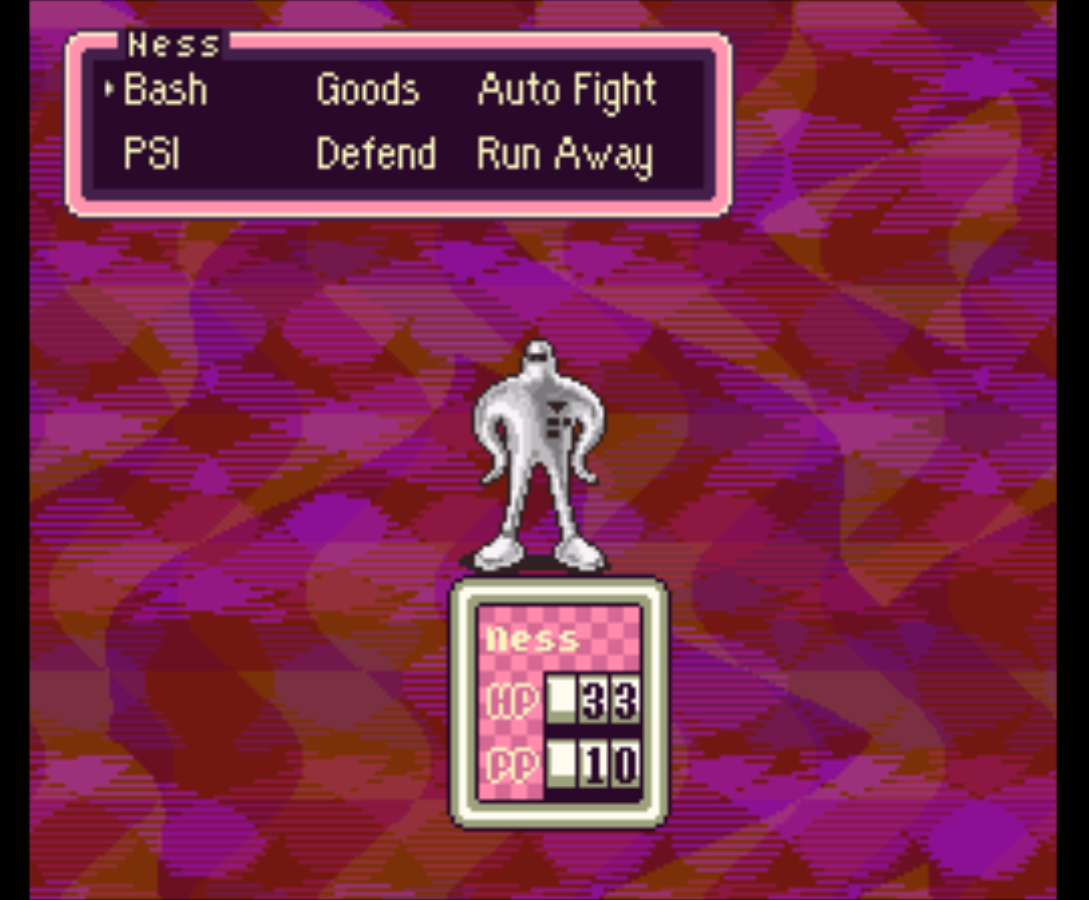
\includegraphics[width=9cm]{figures/Earthbound.png}
  \caption{A screenshot of a battle from the turn-based role-playing game \textit{Earthbound} \cite{earthbound94}.}
  \label{fig:Earthbound}
\end{figure}

For instance, observe the battle shown in Figure \ref{fig:Earthbound} from the game \textit{Earthbound}. The computer opponent is shown in the center of the screen. At the top, the actions available to the player are listed. Players have the choice of making a melee attack (Bash), casting a magical spell (PSI), using an item (Goods), or reducing damage taken (Defend). Players can also select Auto Fight to have the computer make all the choices for them, or they can Run Away and escape from the battle. At the bottom, the hit points (HP) and psychic points (PP) of the character are shown - these correspond to the character's health and magical abilities, respectively. Specific to turn-based RPGs, the player has as much time as they want to decide on their strategy. This is in contrast to an action RPG, where combat takes place in real-time. Generally, action RPGs use 3D environments to better accommodate the real-time battles, but this is not always the case.\\

In the game created for this thesis, a turn-based approach is better suited because it emphasizes player strategy. Action RPGs may have similar lists of commands and actions, but these actions frequently have a corresponding skill component. Take for example a basic attack. In a turn-based RPG, this action requires little from the player: they select that choice from a list, and their in-game character attacks the opposing player. Depending on the game, this attack may or may not be successful - the opponent could dodge or block the hit - but the success or failure is determined by the game through the stats of both players. For instance, a character may have a high enough agility to dodge an attack, or a high enough defensive to block the strike; the role-playing aspect of turn-based RPGs often boils down to how players build their character's stats. An action RPG, on the other hand, determines whether an attack misses or hits through hit-boxes. A hit-box is a hidden area tracked by the game code and tied to some in-game object; when hit-boxes intersect, something happens depending on the types of objects. For this example, an attack would be successful if the hit-box of the character's attack (their sword, fist, magic spell, etc.) intersects with the hit-box of their opponent's body. The attack would fail if these hit-boxes do not intersect. Thus, the overall success of a character in an action RPG is dependent on a player's skill in making hit-boxes collide. This type of gameplay does not lend itself well to game theory analysis, as a player could make all the right decisions but still lose from lack of skill.\\

\begin{figure}[H]
  \centering
  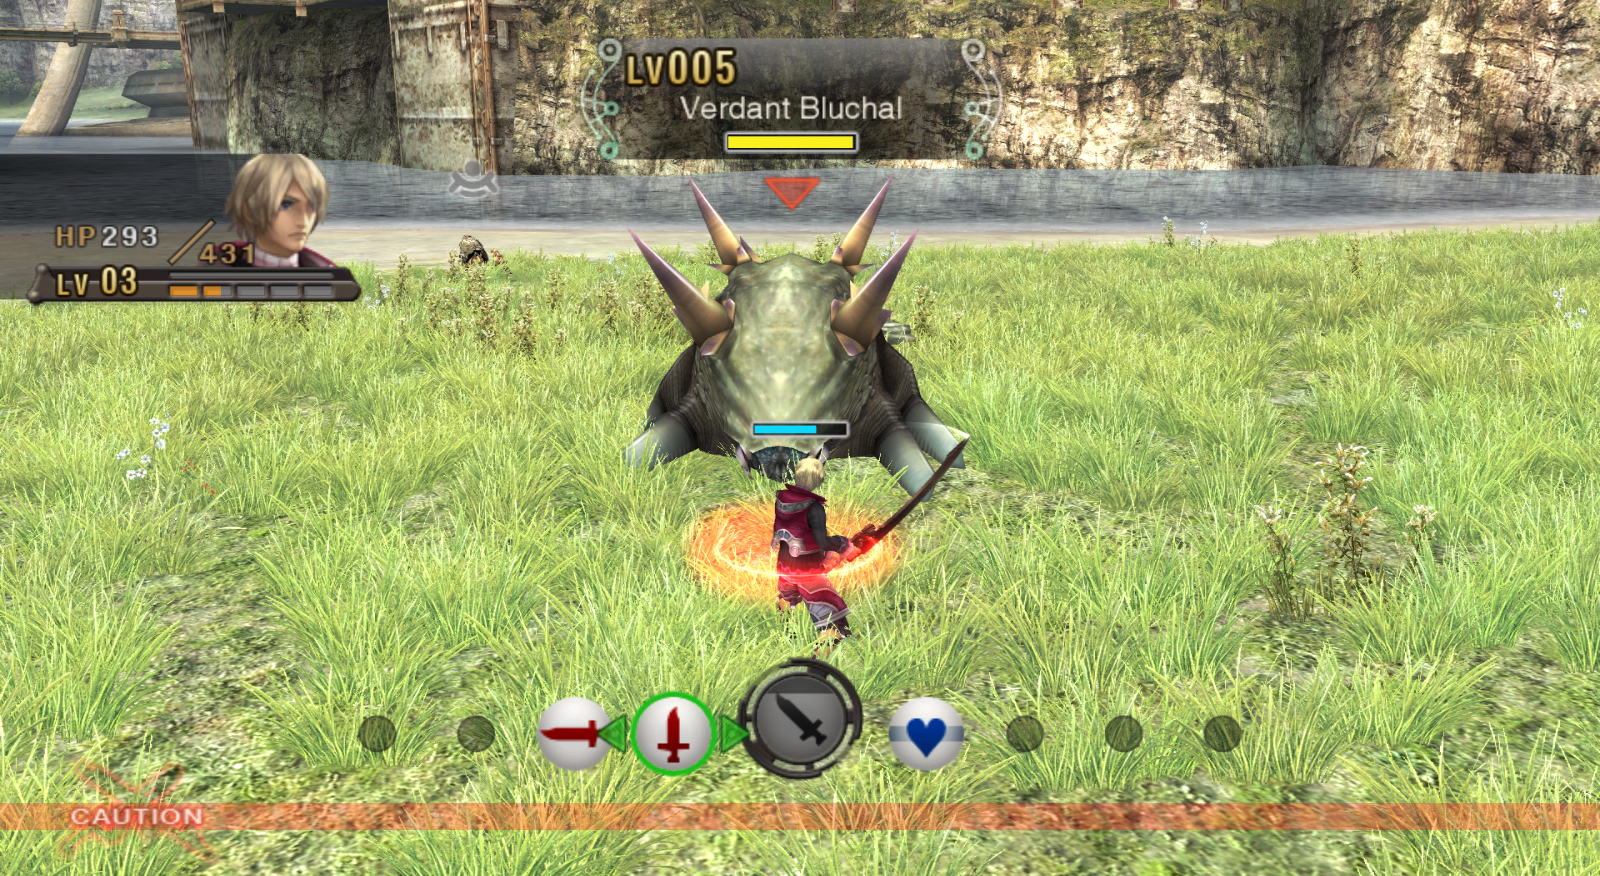
\includegraphics[width=11cm]{figures/Xenoblade.png}
  \caption{A screenshot of a battle from the action role-playing game \textit{Xenoblade Chronicles} \cite{xenoblade10}.}
  \label{fig:Xenoblade}
\end{figure}

For a more concrete example, regard a battle from the action RPG \textit{Xenoblade Chronicles}, as shown in Figure \ref{fig:Xenoblade}. In this game, the player can move freely in 3D space. The character shown currently has four abilities, represented as icons along the bottom of the screen. The two red-tinted abilities are attacks, as is the shaded center ability. The blue ability on the right is a healing spell. The skill component of this game comes with the two red abilities; these abilities do more damage and cause additional effects when performed at certain angles. For instance, the leftmost ability reduces an opponent's defense when used on the enemy's side, while the second red ability does more damage when used from an opponent's back. Thus, two players could use the same series of abilities but have different outcomes based on how their attacks were positioned.\\

Similarly, the game presented in this thesis is a two-dimensional game. With a turn-based RPG, since the gameplay involves choosing actions from a list, the only difference between a 2D and a 3D turn-based RPG is the graphical quality. A 2D game uses sprites, while 3D games use polygonal models. A two-dimensional game was chosen to simplify development.\\

To begin building an AI model, we first create a simulation of the \textit{Cave Escape}. The simulation has two players, each with 25 health points (HP). In this first simulation, both players have two possible actions per turn which are randomly selected: attack the other player, reducing their opponents HP by 5 points, or heal themselves, increasing their HP by 4 points. Players can not heal above their starting value of 25 HP; any extra health points are discarded. Each action has a 50\% chance of occurring. The game runs until one player's HP is reduced to 0. The total number of turns and the sequence of actions are recorded into a CSV file. Each line of the CSV file contains the length of the game, a sequence of Player 1's HP values, then a sequence of Player 2's HP values. After running 4500 simulations, the data is imported into MATLAB. A subset of the games are used as a training set for a decision tree, which predicts the player that wins the game.\\

\begin{figure}[H]
  \centering
  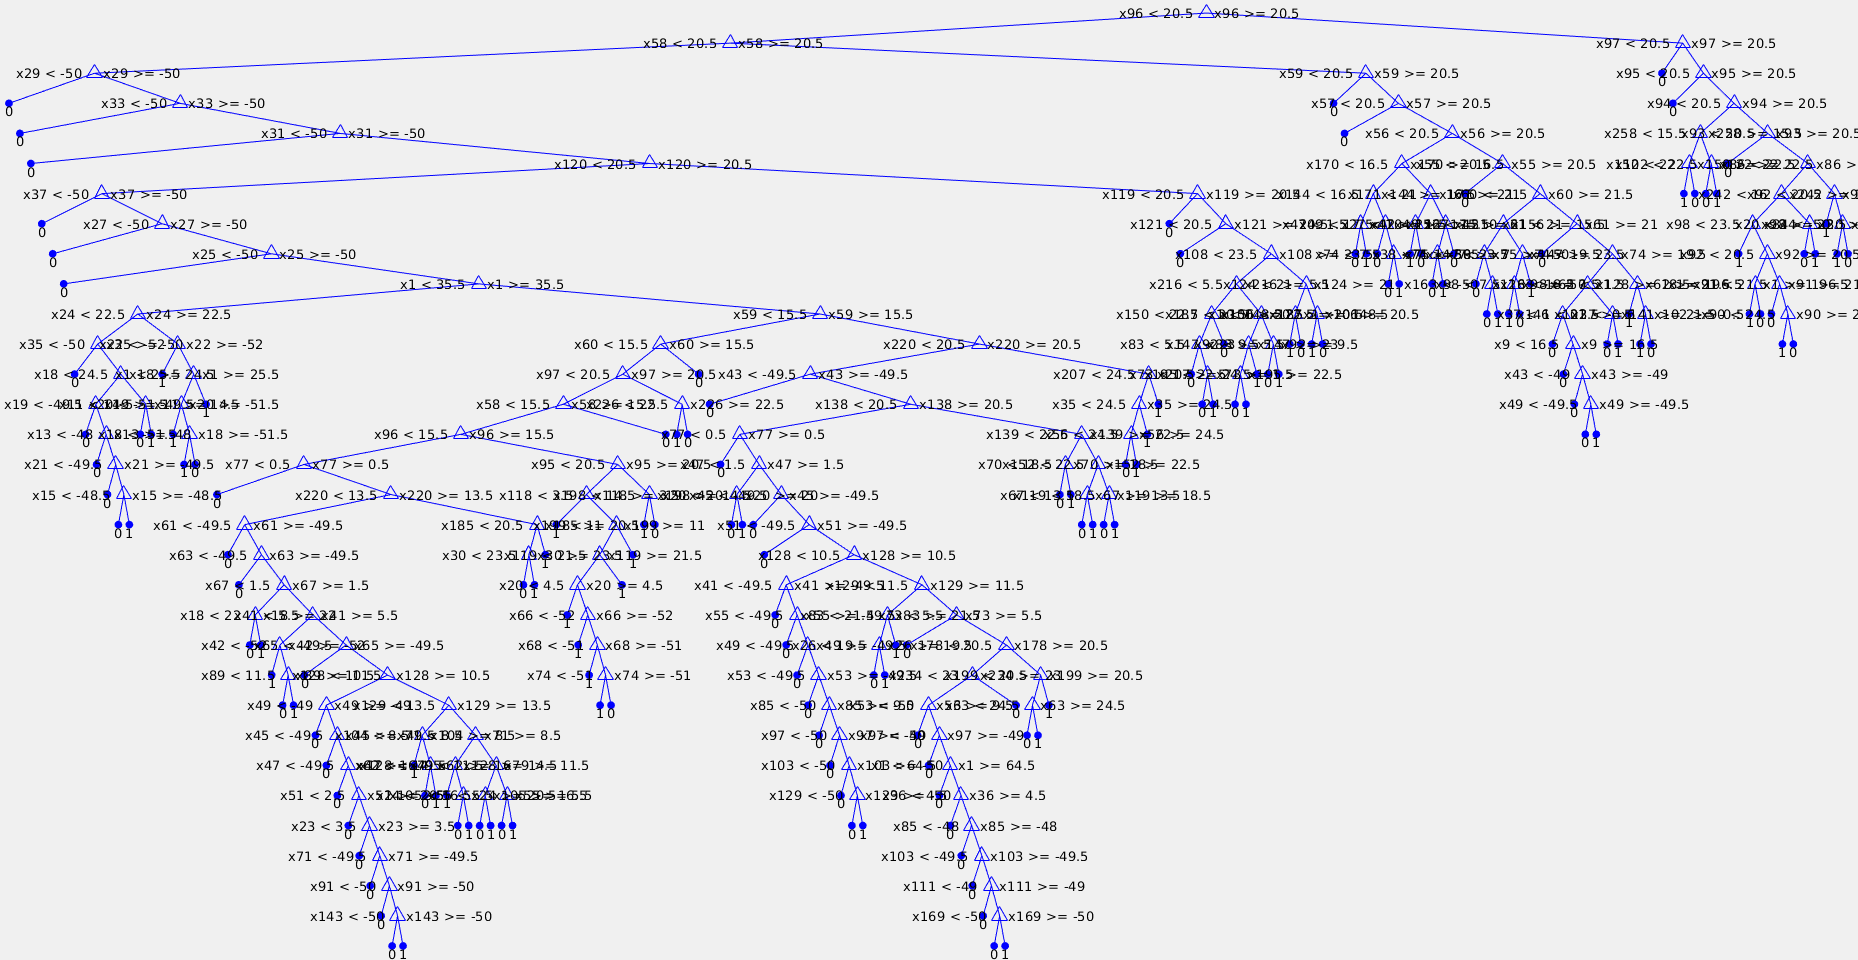
\includegraphics[width=13cm]{figures/firstDecisionTree.png}
  \caption{The decision tree generated from 4000 simulations of the game. The predicted attribute is a Boolean value of 0 when player 1 wins and 1 when player 2 wins.}
  \label{fig:decisionTree1}
\end{figure}

However, this method is inconclusive, for a number of reasons. Firstly, the decision tree includes a  large number of branches, as seen in Figure \ref{fig:decisionTree1}. Secondly, the actual criteria evaluated at each branch of the tree is different for each game. Aside from the first column, which contains the total number of turns in the game, and the second column, which contains the starting HP of player 1, the values in any particular column differ from game to game. For instance, the root node uses the value in column 96 as its classifier. In one game, column 96 may contain a HP value for Player 2. In another, longer game, that column may contain a HP value for Player 1. Thirdly, the individual games contain numerous streaks: a longer game is not the result of better strategy, but is instead caused by streaks where both players choose to heal on their turns. Players in these streaks reach HP levels near the 25 HP cap, effectively resetting the game.

The lack of consistency along columns is most likely the largest detriment to this model. Decision trees work best when classifying problems on specific attributes; if the attribute is different at column 96 from one game to another, the information gain at that column is meaningless. This is likely behind the sprawling nature of the decision tree itself. Without clear attributes to test, each split only has minuscule amounts of information gain.

\subsection{Extensive Tree Model}
A game theoretic angle is used on the second attempt. The HP of both players is reduced to 10, and two restrictions are added on healing: a player can not heal when they have full health, and a player can only heal themselves twice. As in the first attempt, players can only attack or heal. With these new rules in place, we create an extensive-form tree for the new game.\\

\begin{figure}[H]
  \centering
  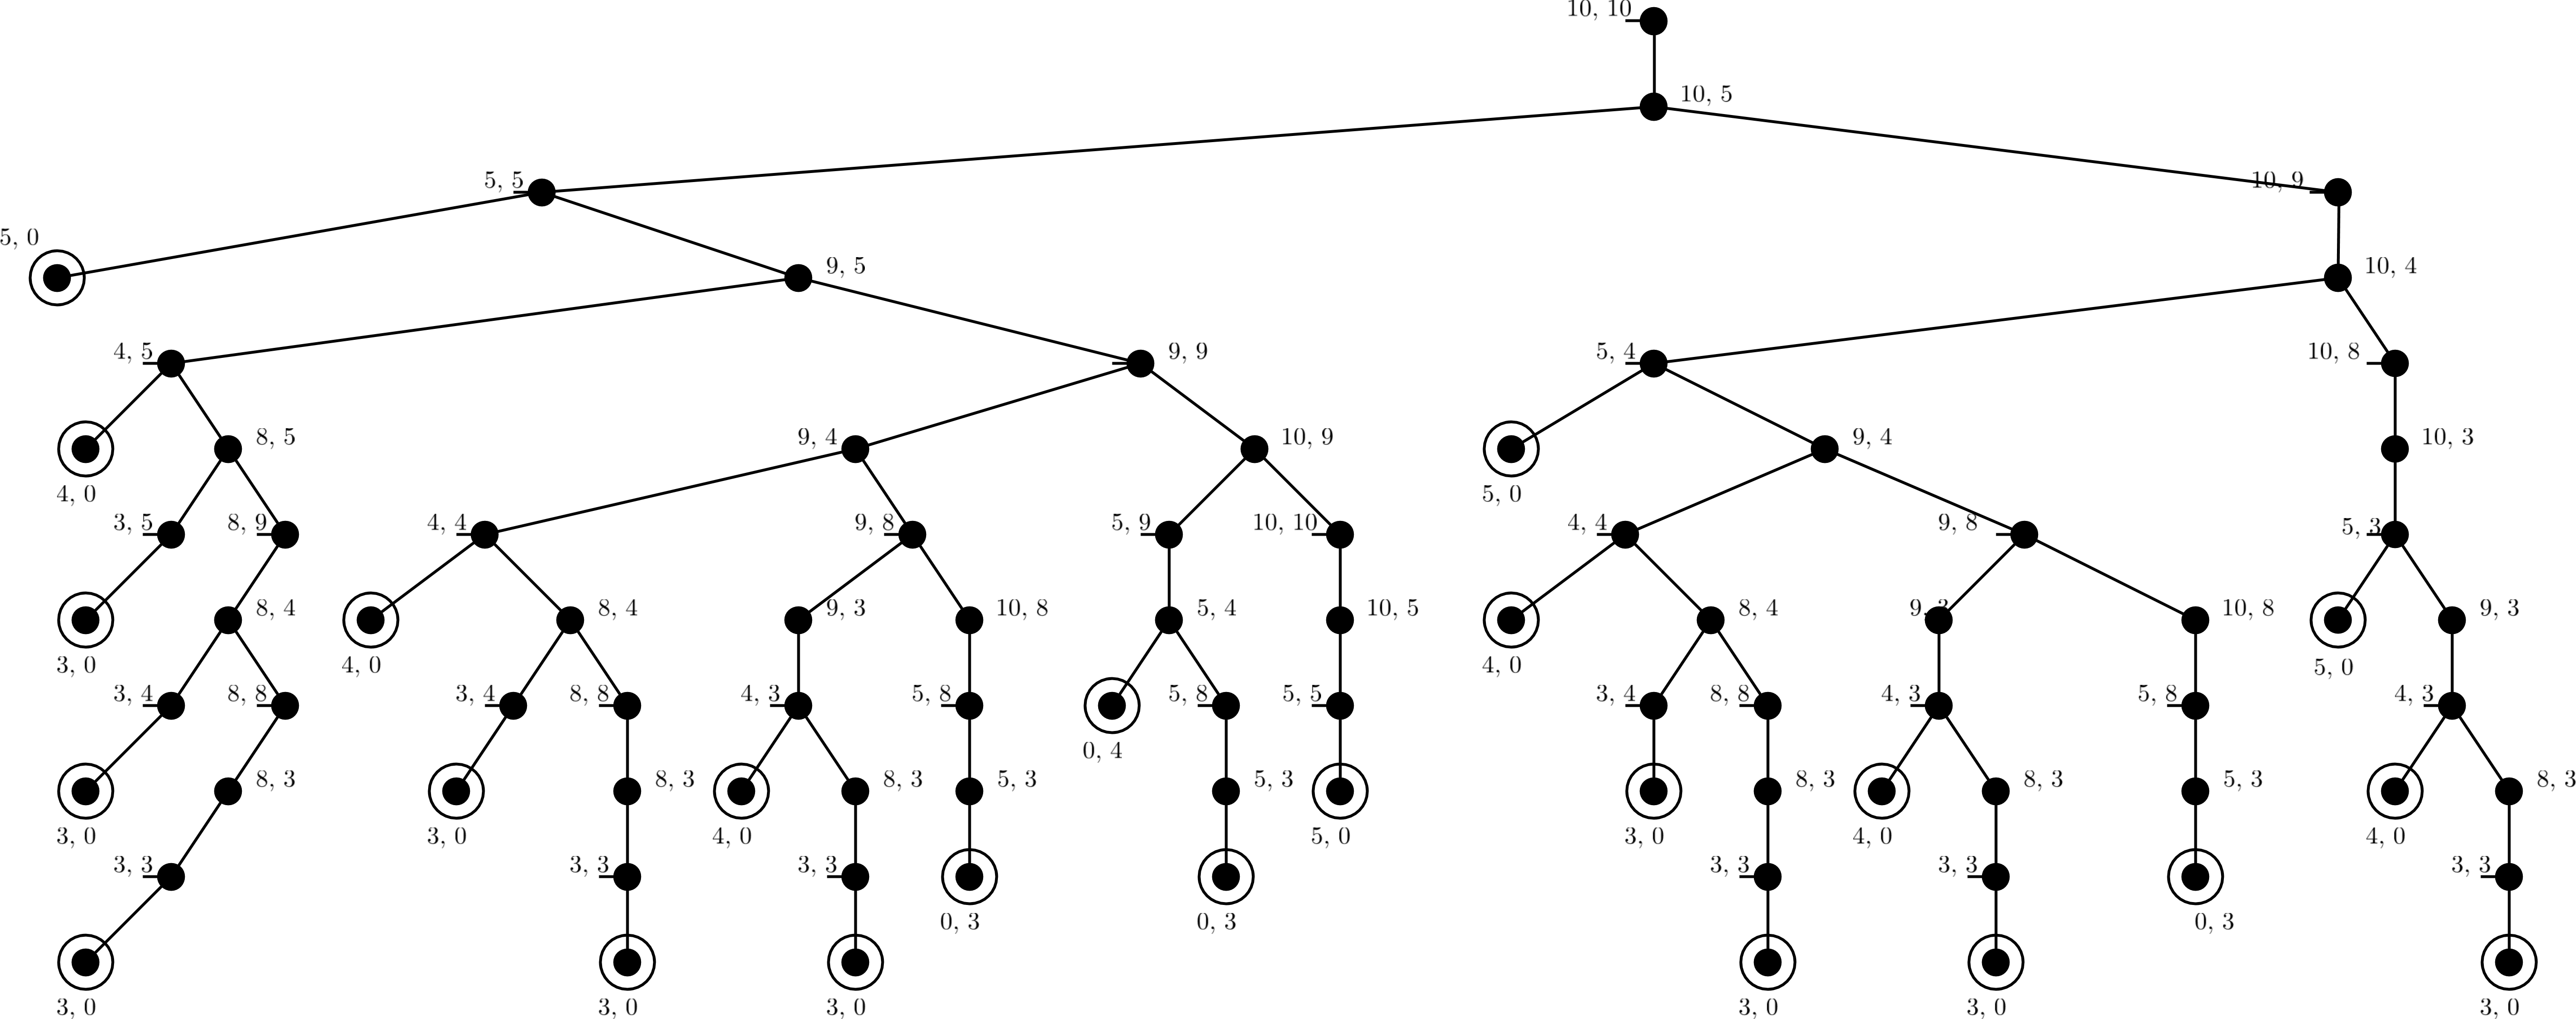
\includegraphics[width=14cm]{figures/GameTree.png}
  \caption{The extensive-form tree for a simplified game. Each player starts with 10 hit points (HP). At each node, a player can choose to heal themselves or attack their opponent. Attacking reduces the opponent's HP by 5 points. Healing increases the decision maker's HP by 4 points; they can only heal themselves twice per game.}
  \label{fig:gameTree}
\end{figure}

In Figure \ref{fig:gameTree}, Player 1's nodes are denoted by a small dash to the left of the node. The HP values of both players are recorded at each node. Leaf nodes where Player 1 wins are enclosed in a circle, and leaf nodes where Player 2 wins are enclosed in a diamond. There are 24 outcomes for this game; of these, only 4 of them result in a win for Player 2, while the other 20 result in wins for Player 1. In fact, with optimal play, Player 1 always wins in this game.\\

\begin{figure}[H]
  \centering
  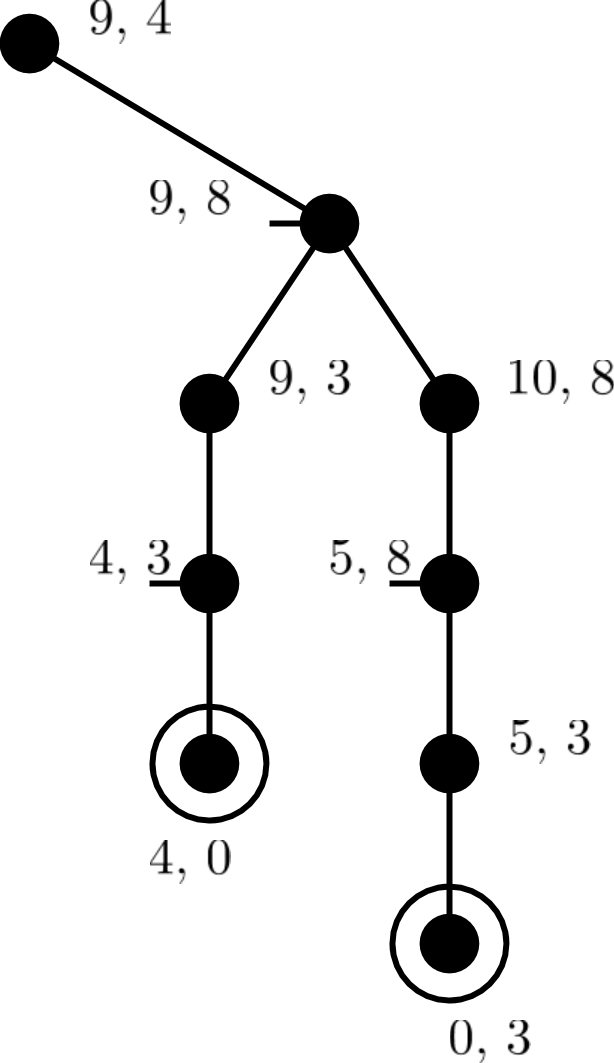
\includegraphics[width=3.5cm]{figures/GameSubtree.png}
  \caption{A subtree of the extensive-form representation in Figure \ref{fig:gameTree}. This subtree contains one of player 2's only winning outcomes.}
  \label{fig:gameSubtree}
\end{figure}

For example, in the subtree shown in Figure \ref{fig:gameSubtree}, both players have a winning outcome. However, the critical decision is made by Player 1. If Player 1 chooses to heal at the root of this subtree, then Player 2 will win in 3 more turns. If Player 1 chooses to attack, then Player 1 will eventually win. Thus, in any game which reaches this subtree, Player 1 will choose to attack on their turn since that choice leads to their victory.\\

\begin{figure}[H]
  \centering
  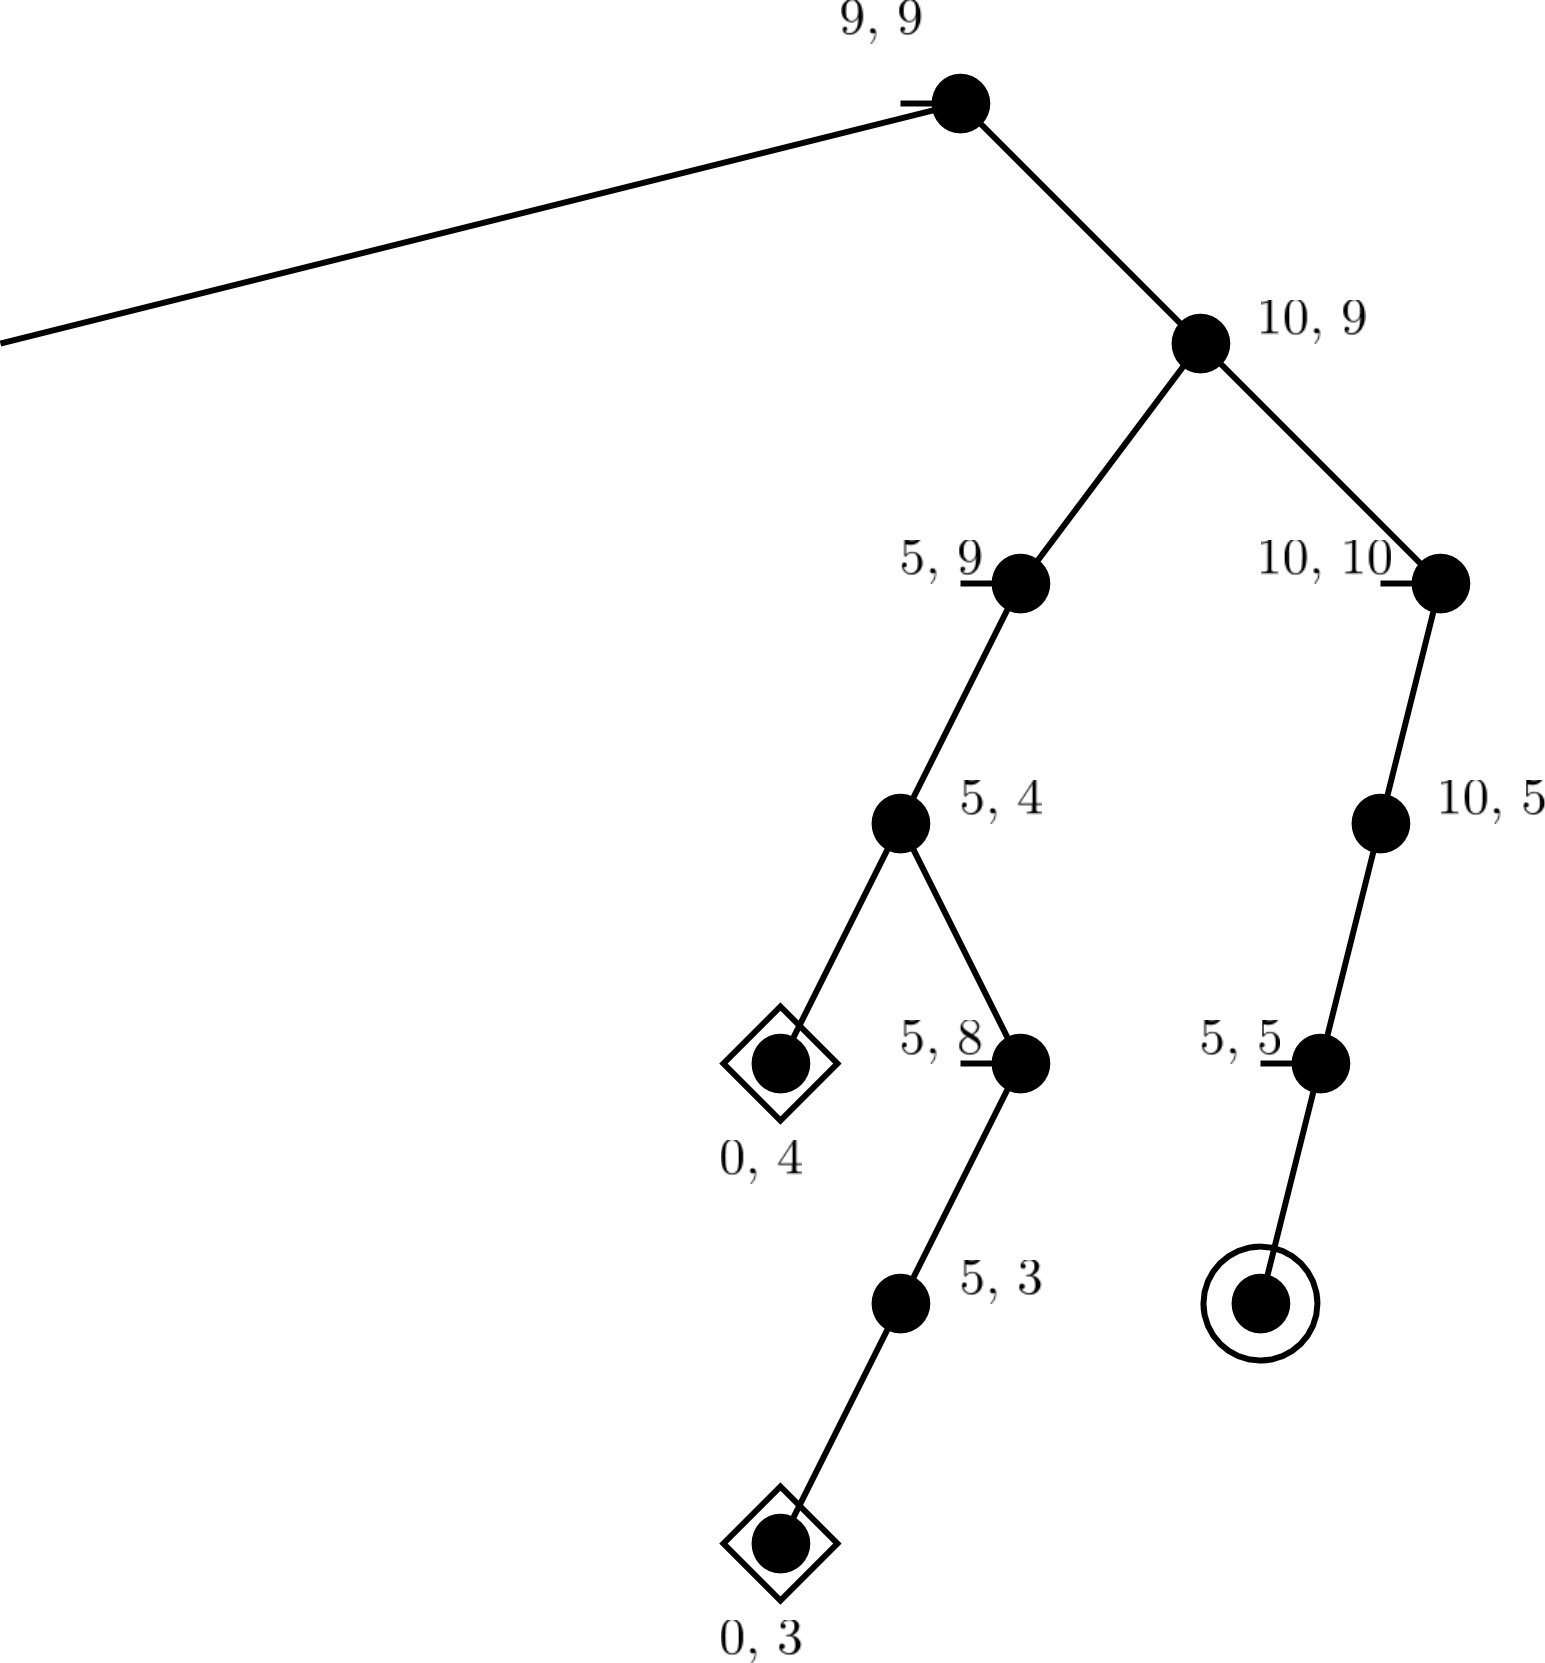
\includegraphics[width=6cm]{figures/GameSubtree2.png}
  \caption{A second subtree of the extensive-form representation in Figure \ref{fig:gameTree}. This subtree contains two more of player 2's winning outcomes.}
  \label{fig:gameSubtree2}
\end{figure}

Two more of Player 2's winning outcomes can be seen in the subtree in Figure \ref{fig:gameSubtree2}. At the root node of this subtree, Player 1 is making their choice. If they choose to heal, the game moves into the right child. Player 2's first choice on the right child's subtree either results in a win (if Player 2 attacks) or a loss (if Player 2 heals). Thus, an intelligent Player 2 would always attack at this stage, since it is a guaranteed win. However, if Player 1 knows that this is a guaranteed win for their opponent, Player 1 can avoid this threat by attacking instead of healing at the root node.\\

If Player 1 decides to avoid the subtree in Figure \ref{fig:gameSubtree2}, Player 2 has the next choice. If Player 2 decides to heal at this new node, then the resulting subtree is identical to the one found in Figure \ref{fig:gameSubtree}. This subtree contains Player 2's final winning outcome, but once again Player 1 can avoid this outcome with ease.\\

\subsubsection{Backwards Induction on Extensive Tree Model}
We can prove that Player 1 will always win this game through the backwards induction algorithm discussed in Chapter 2. Recall that the algorithm travels through a game tree by recursion and, at each node, returns the child node which gives the player acting at the parent node the most utility.

\begin{figure}[H]
  \centering
  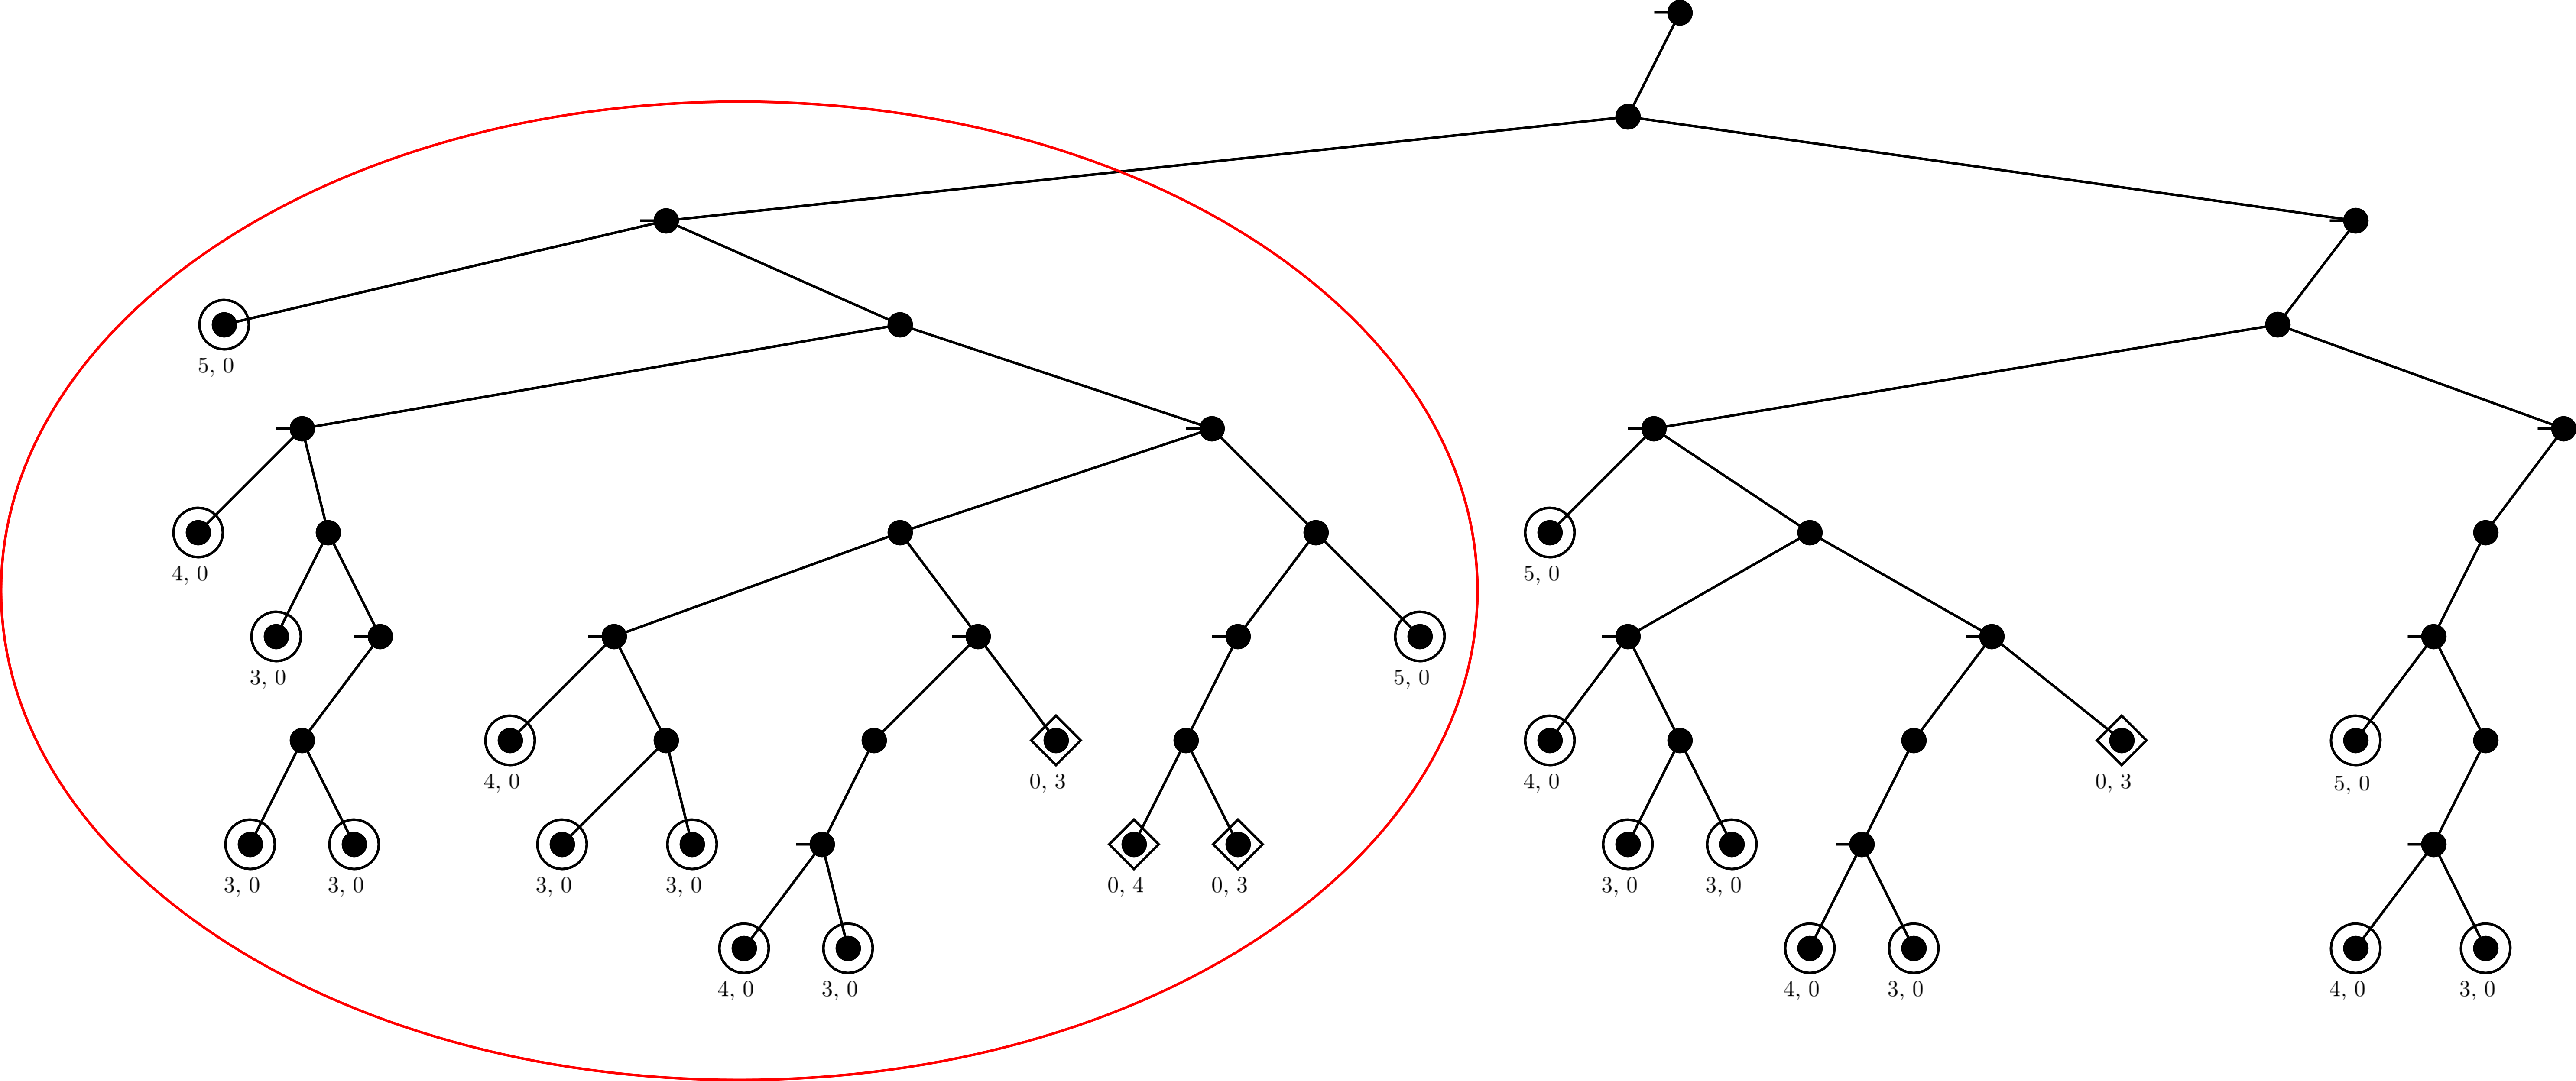
\includegraphics[width=13cm]{figures/Backwards0.png}
  \caption{The extensive-form tree for the simplified version of the game, but with extraneous nodes removed; a node is extraneous if the player making their decision has only one possible action. The circled subtree will be the first subtree examined on recursive calls of the backwards induction algorithm.}
  \label{fig:condensedTree}
\end{figure}

For the example in Figure \ref{fig:gameTree}, we can trivially condense branches where only one action is available, taking the utility values from the leaf nodes and copying them up the tree. This produces the tree seen in Figure \ref{fig:condensedTree}. We define the utility of a player in this game as their HP at the end of the game minus the HP of their opponent. Thus, for a game with the outcome (4, 0), Player 1 will have a utility of 4 and Player 2 will have a utility of -4.\\

The algorithm begins at the root node of the tree. Since the root is not a leaf node, the algorithm is called on the root's children, starting with the leftmost child. The root node only has one child, since players cannot heal when their HP is maxed out. So, the backwards induction algorithm is called on the next node, which does have more than one child. To find the utility of both children, the algorithm must be recursively called on both subtrees, starting with the subtree circled in red in Figure \ref{fig:condensedTree}.\\

\begin{figure}[H]
  \centering
  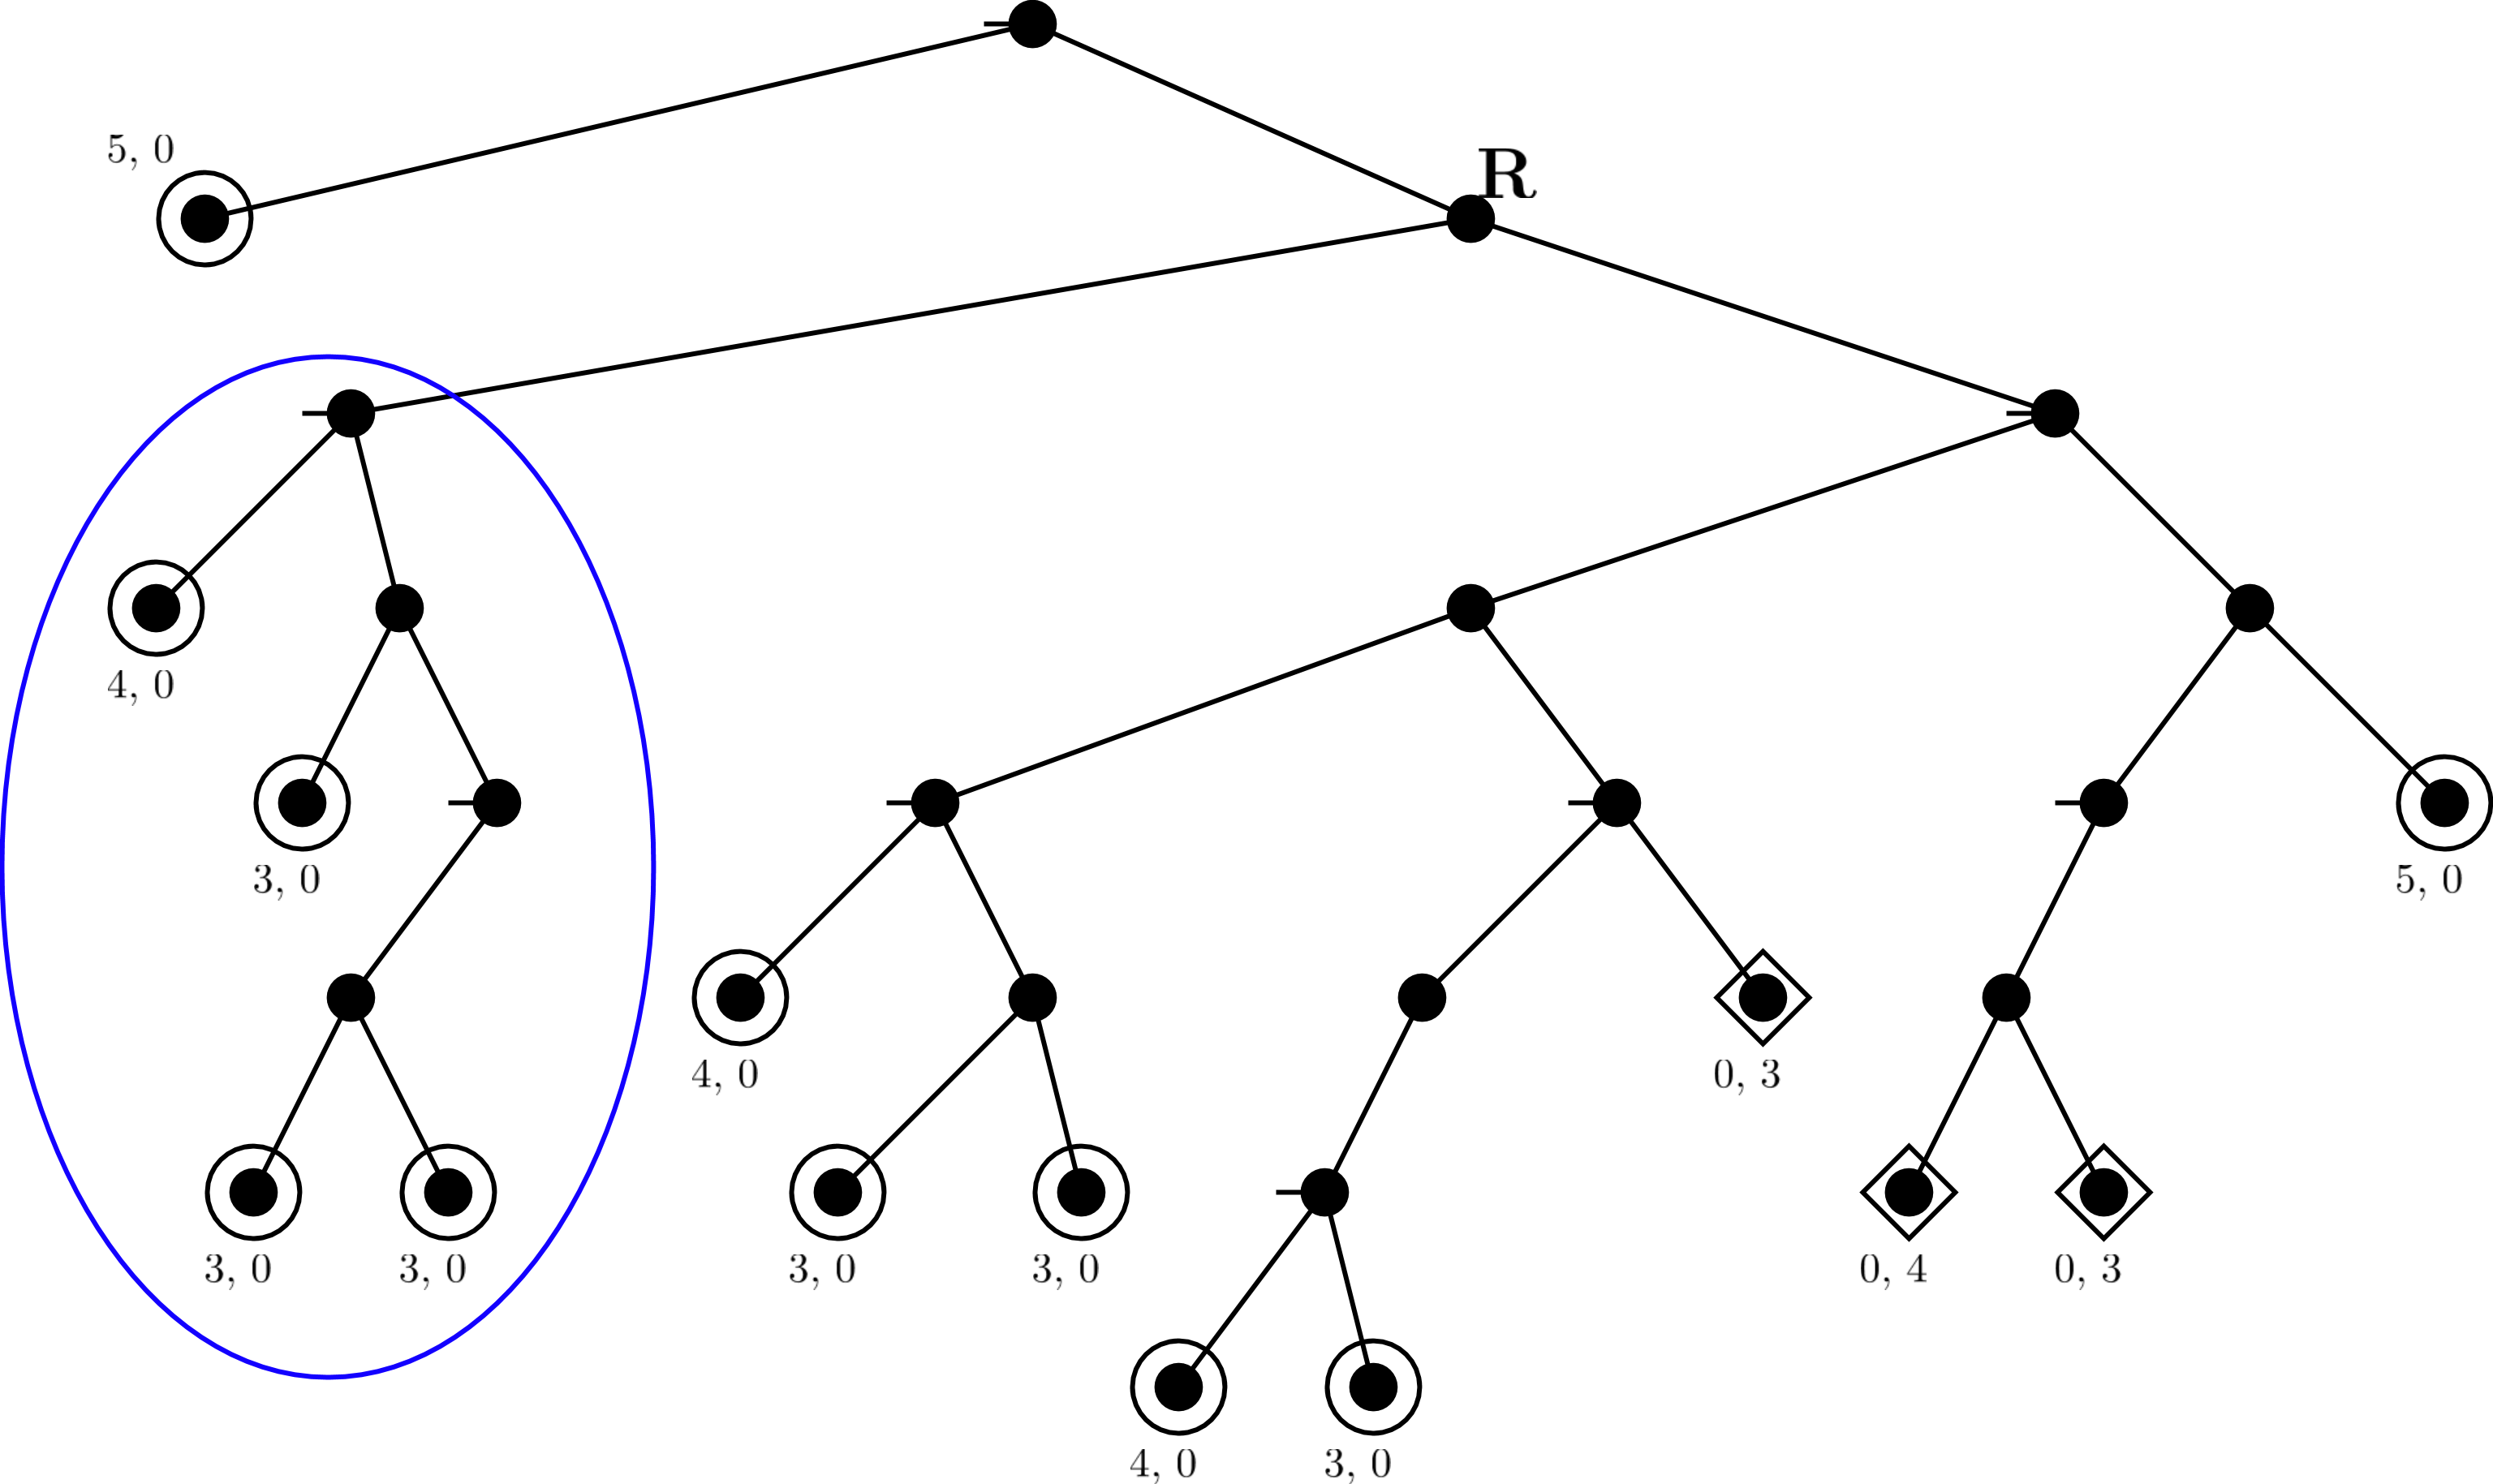
\includegraphics[width=11cm]{figures/Backwards1.png}
  \caption{The tree examined by the backwards induction algorithm after recursing to the red circled subtree in Figure \ref{fig:condensedTree}. The blue circled subtree is the next recursive step of the algorithm.}
  \label{fig:backwards1}
\end{figure}
Examining the root of the subtree in Figure \ref{fig:backwards1}, we find that the left child of the root is a leaf node. Thus, since the root is a decision node for Player 1, the utility of this entire subtree will be the maximum utility for Player 1 between the leaf node (5, 0) and the utility of the right child, which is its own subtree. Once again, the backwards induction algorithm is called recursively, this time on the subtree with root $R$. On the recursive call, the left child of $R$ is the subtree circled in blue.\\

\begin{figure}[H]
  \centering
  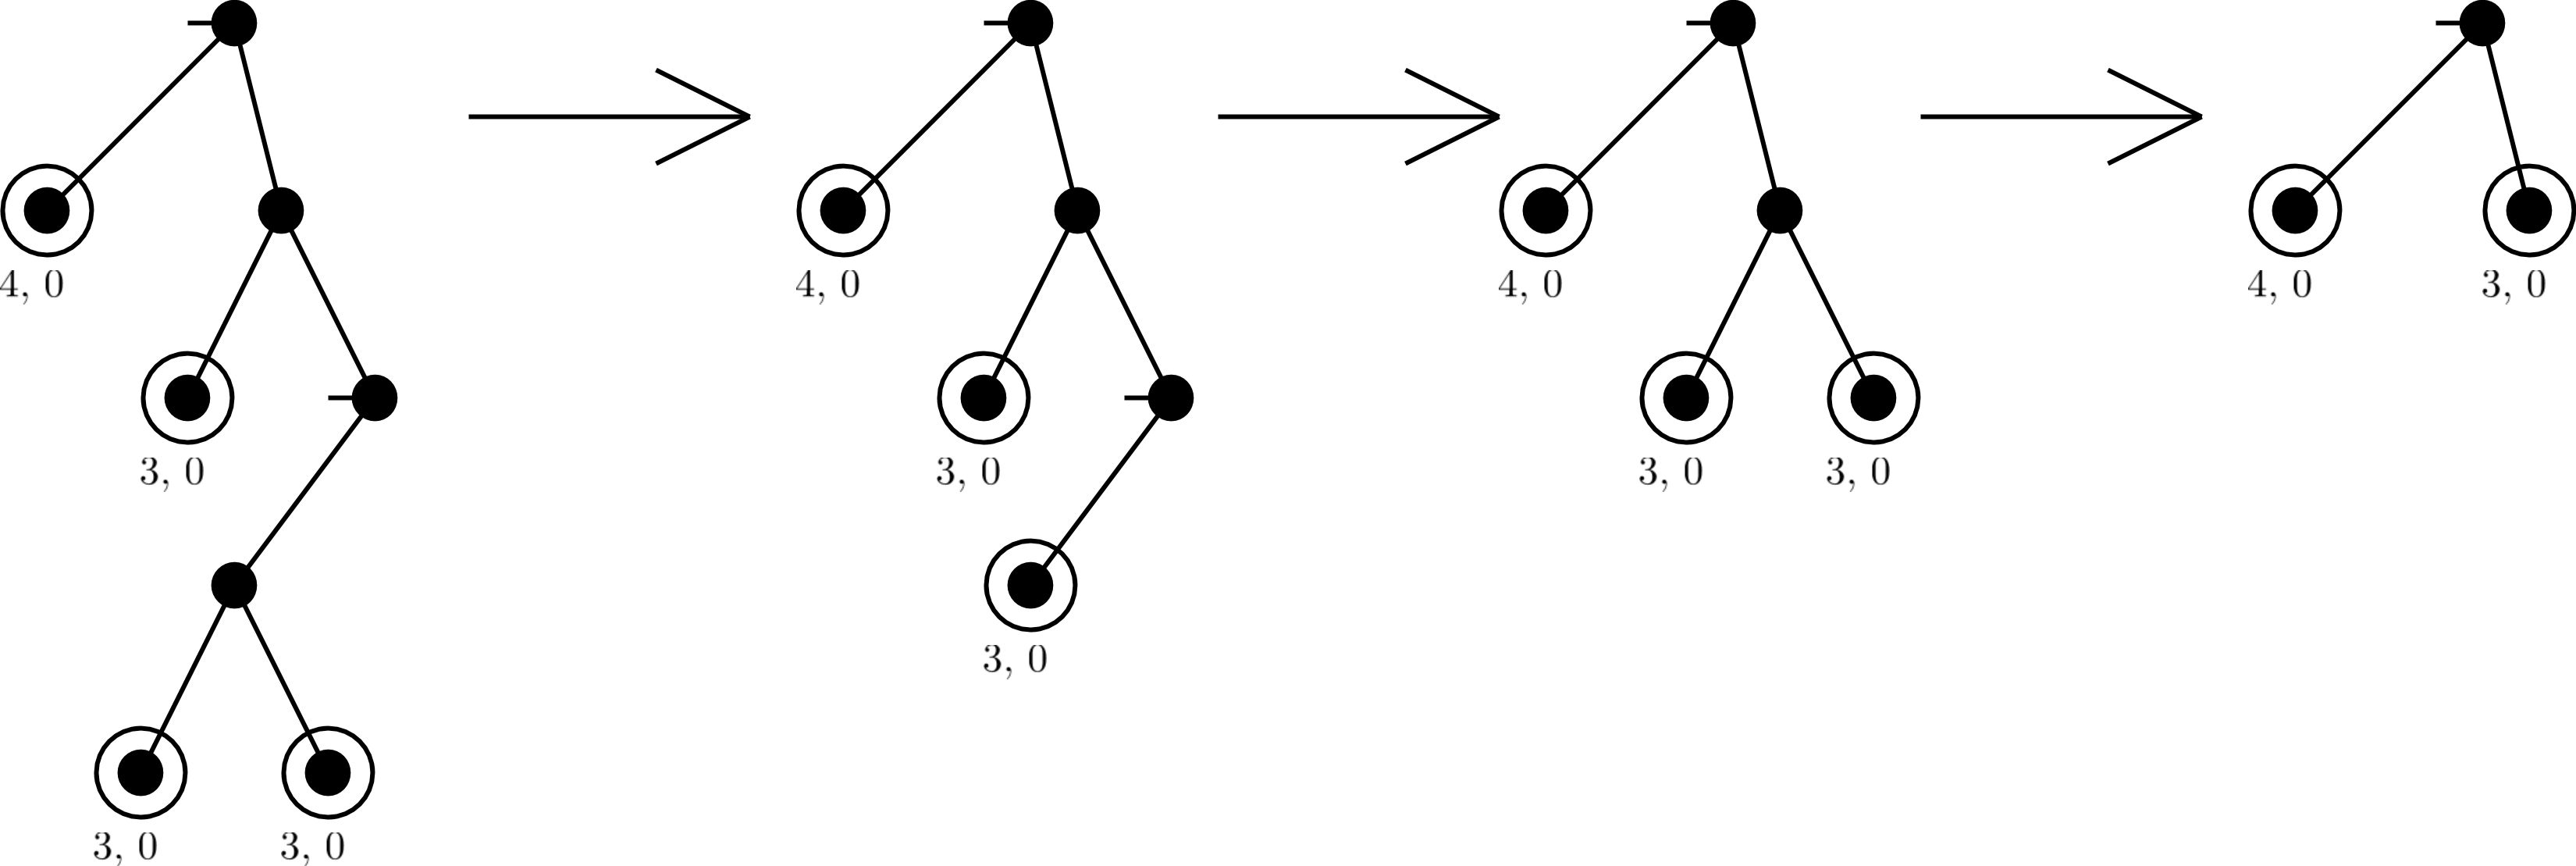
\includegraphics[width=12cm]{figures/Backwards2.png}
  \caption{The steps taken by the backwards induction algorithm after reaching the circled subtree in Figure \ref{fig:backwards1}.}
  \label{fig:backwards2}
\end{figure}
As the algorithm continues to recurse through the game tree, it will eventually reach the pair of leaf nodes at the bottom of the leftmost tree in Figure \ref{fig:backwards2}. The preceding decision node is a choice for Player 2, so Player 2 will make whichever choice gives them more utility. In this example, both leaf nodes provide Player 2 with -3 utility, so the utility of the decision node is (3, 0). This utility value is moved up the tree to the next decision node, as shown in Figure \ref{fig:backwards2}. These steps continue up the subtree. The next decision node again has a tie between (3, 0) and (3, 0), but the root of the subtree has a choice between (3, 0) and (4, 0). Since the root of this subtree is a decision node for Player 1, that player will prefer to attack and reach the (4, 0) leaf node for 4 utility. Thus, the utility of the circled subtree in Figure \ref{fig:backwards1} is (4, 0).\\

\begin{figure}[H]
  \centering
  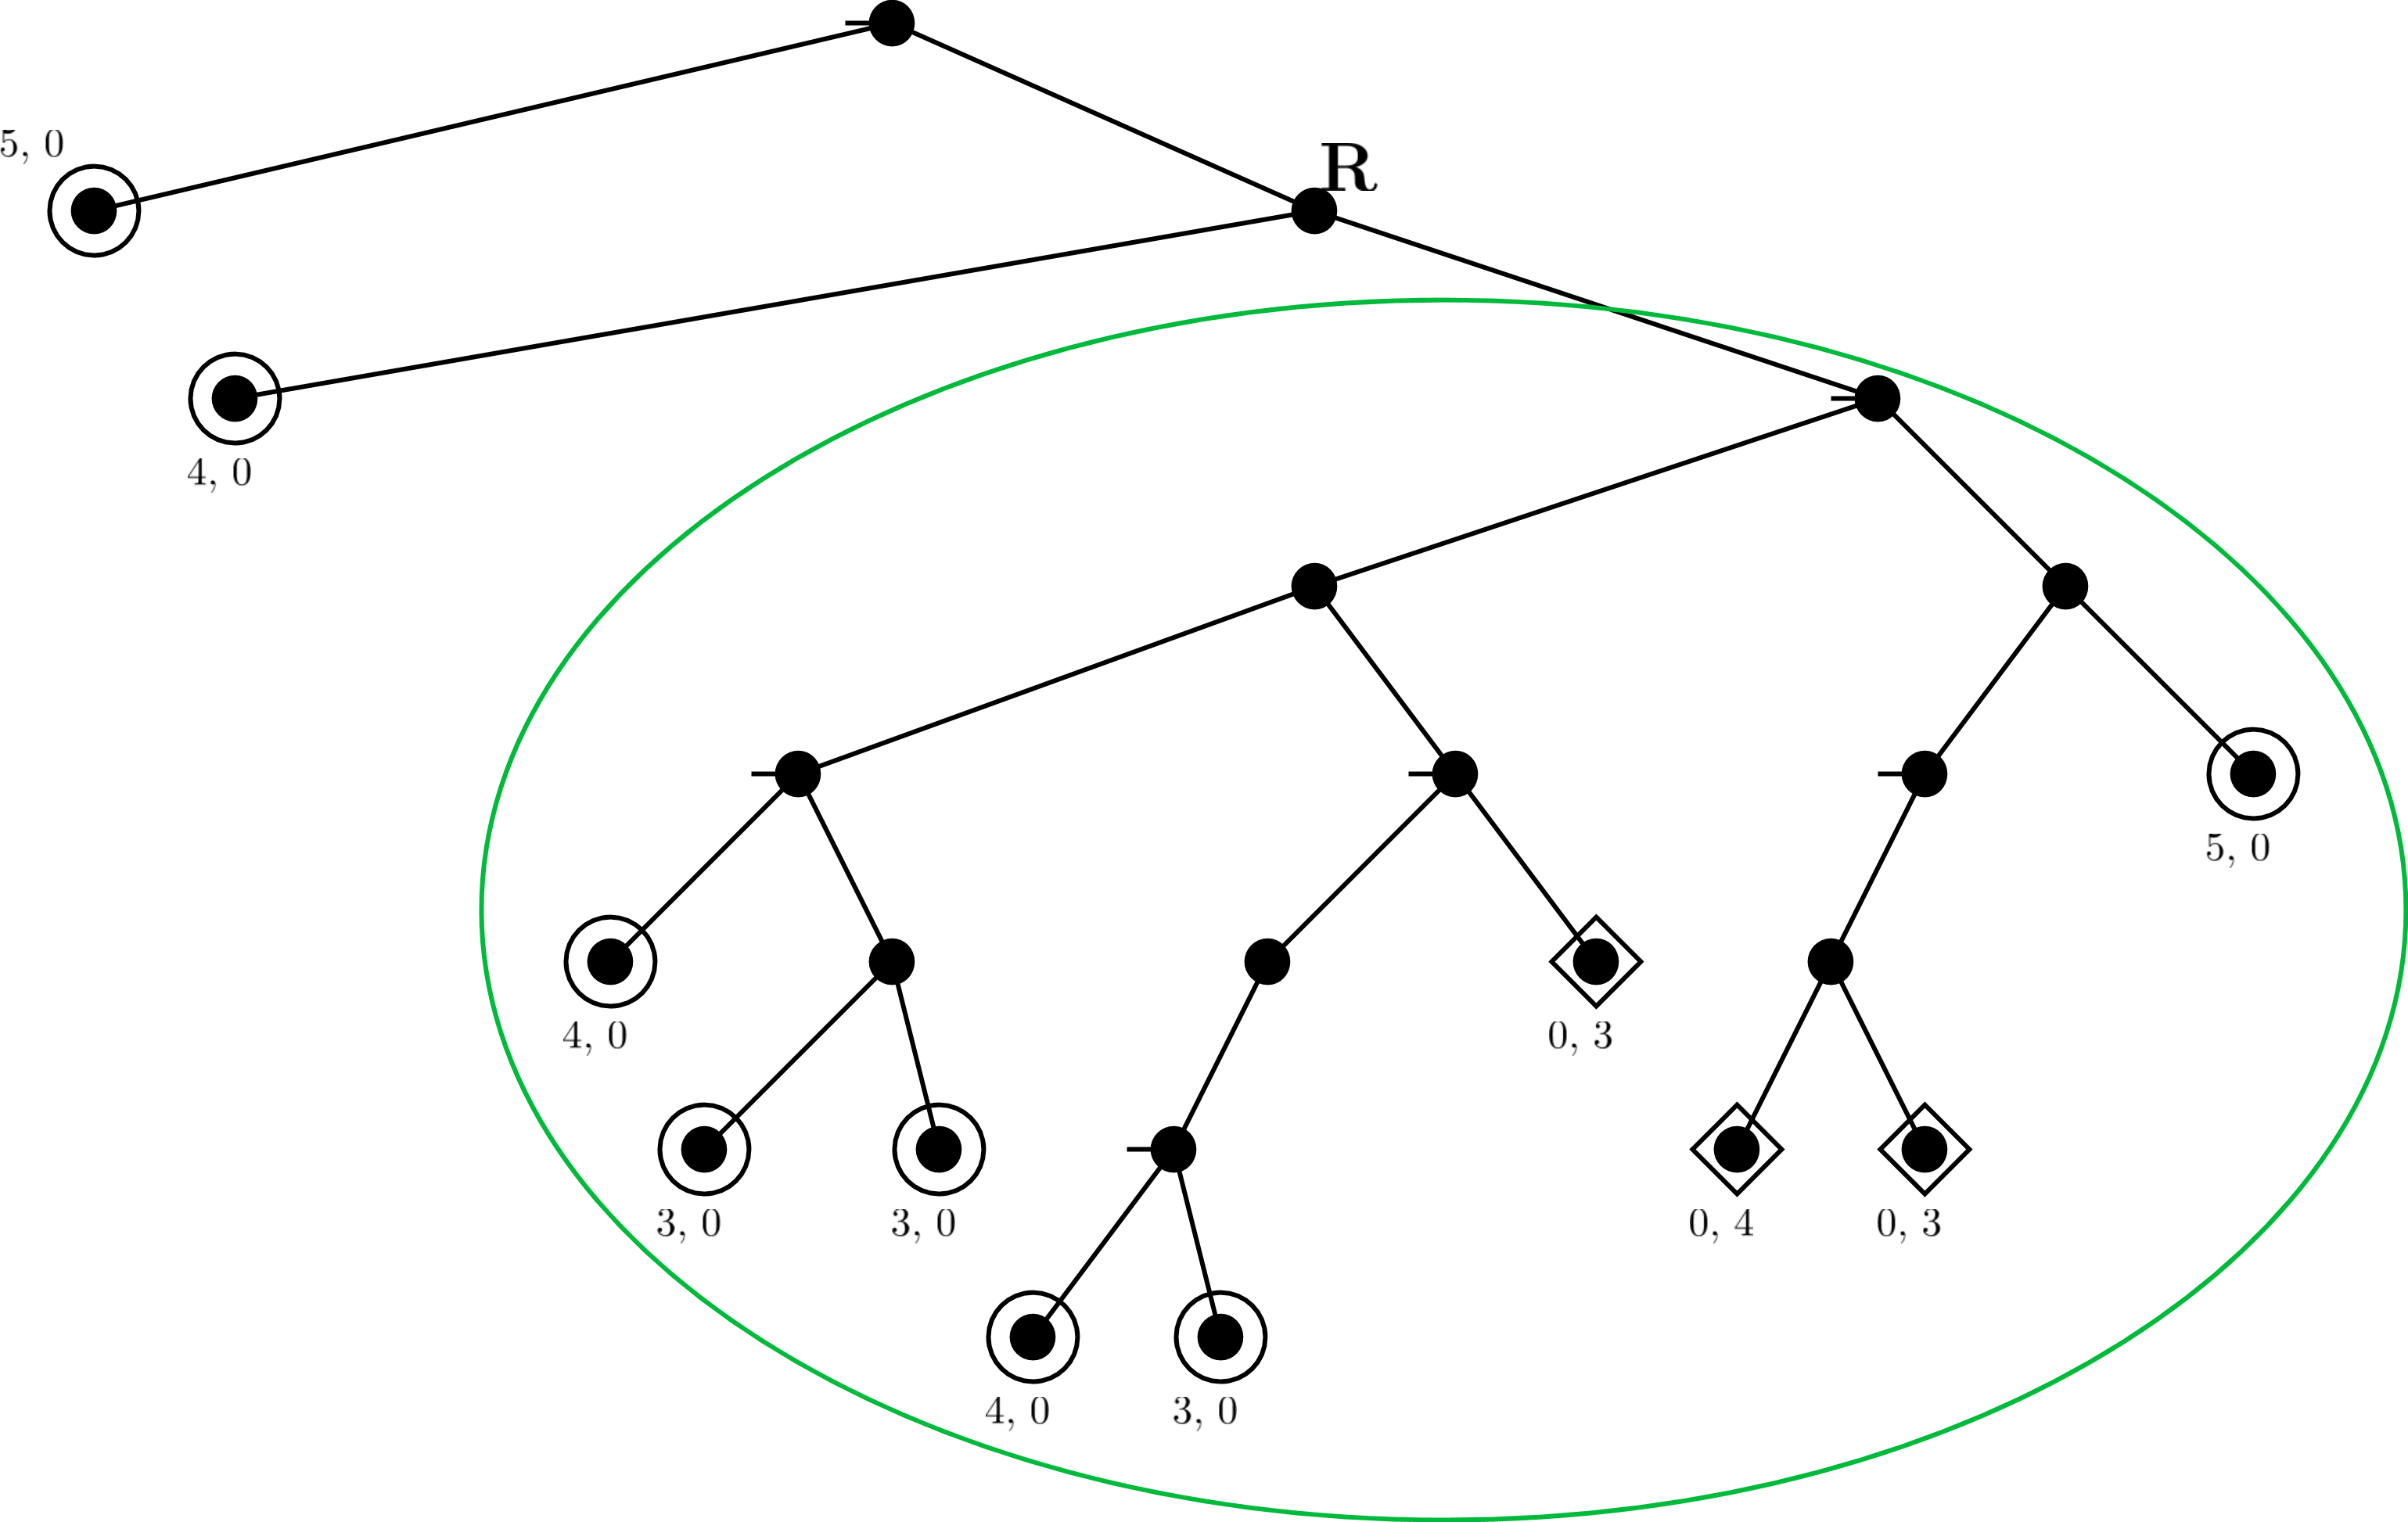
\includegraphics[width=10cm]{figures/Backwards3.png}
  \caption{The subtree in Figure \ref{fig:backwards1}, after the backwards induction steps performed in Figure \ref{fig:backwards2}.}
  \label{fig:backwards3}
\end{figure}

Thus, after exploring the subtree in Figure \ref{fig:backwards2}, the left child of node $R$ is changed from a subtree to a single leaf node, the leaf with utility (4, 0). Now that the left child of $R$ is a leaf node, the algorithm continues along the right subtree of $R$, circled in green.\\

\begin{figure}[H]
  \centering
  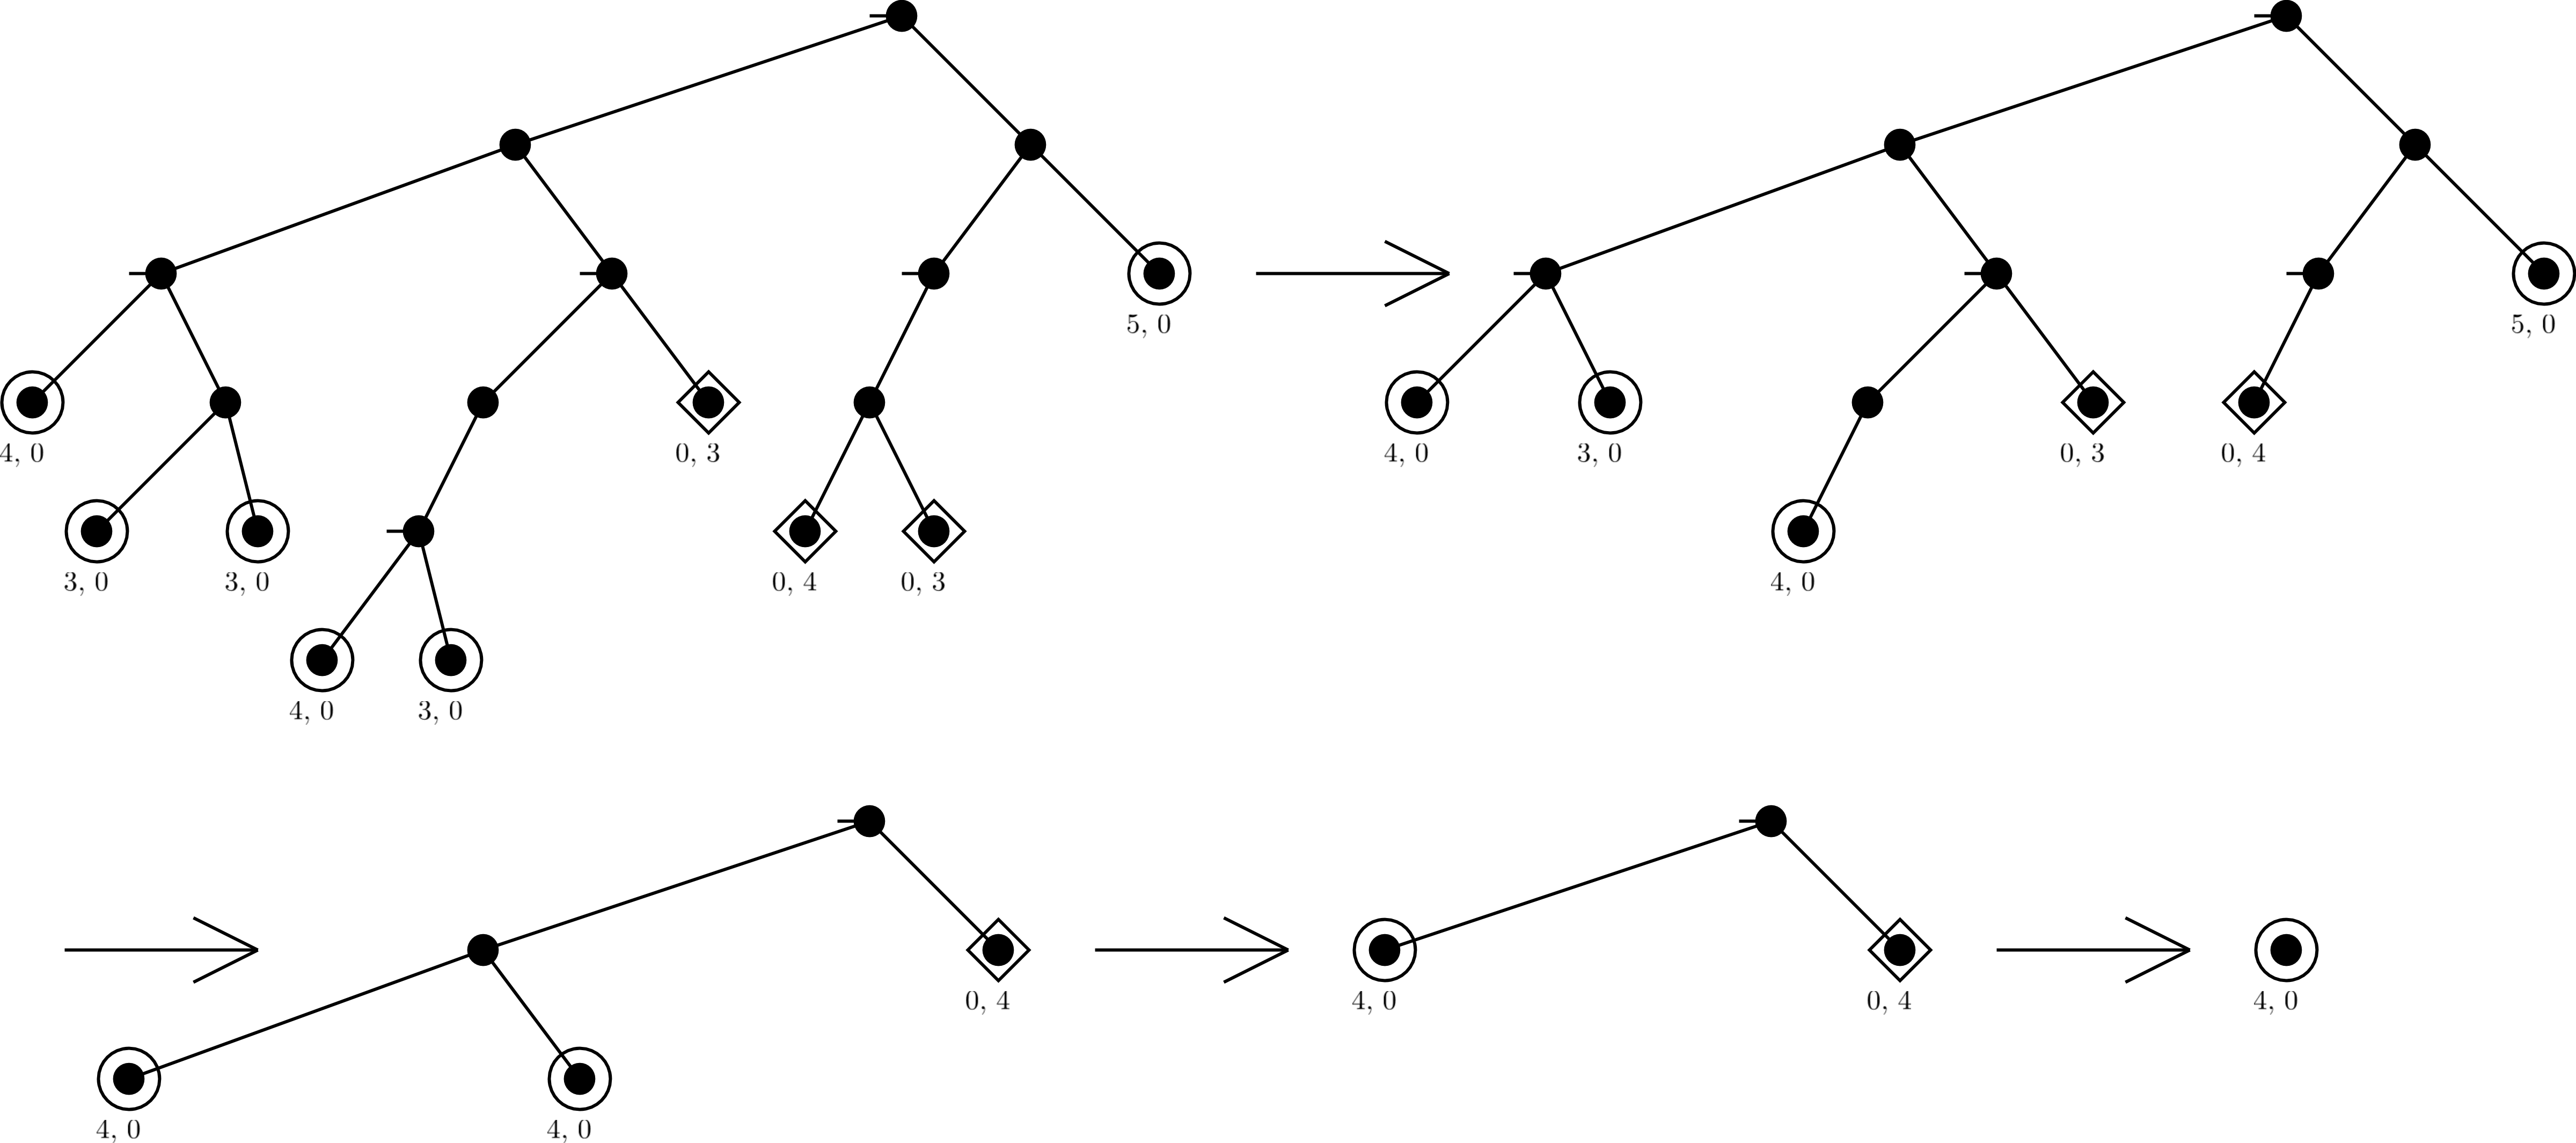
\includegraphics[width=13cm]{figures/Backwards4.png}
  \caption{The steps taken by the backwards induction algorithm after reaching the circled subtree in Figure \ref{fig:backwards3}.}
  \label{fig:backwards4}
\end{figure}

In the new subtree, the induction algorithm again determines which of the leaf nodes to bring up the tree. The parent of the leaf nodes decides which leaf provides the most utility for that player. In the first step, along the bottom of the tree and from the left, Player 2 makes a choice between (3, 0) and (3, 0); Player 1 makes a choice between (4,0) and (3, 0); Player 2 makes a choice between (0, 4) and (0, 3). Respectively, the algorithm chooses (3, 0), (4, 0), and (0, 4). Each of these best leaf nodes are moved up the tree, resulting in the second tree in Figure \ref{fig:backwards4}. From here, extraneous branches are removed and three more decisions are made: player 1 chooses between (4, 0) and (3, 0); Player 1 chooses between (4, 0) and (0, 3); Player 2 chooses between (0, 4) and (5, 0). Respectively, the new utilities of the decision nodes are (4, 0), (4, 0), and (0, 4), creating the third tree in Figure \ref{fig:backwards4}. The next decision is made by Player 2, and is a tie between the two (4, 0) nodes. Then, in the fourth tree shown in Figure \ref{fig:backwards4}, Player 1 makes their choice between the (4, 0) and (0, 4) nodes. Since Player 1 wins on the (4, 0) node, this is the utility of the entire subtree.\\

\begin{figure}[H]
  \centering
  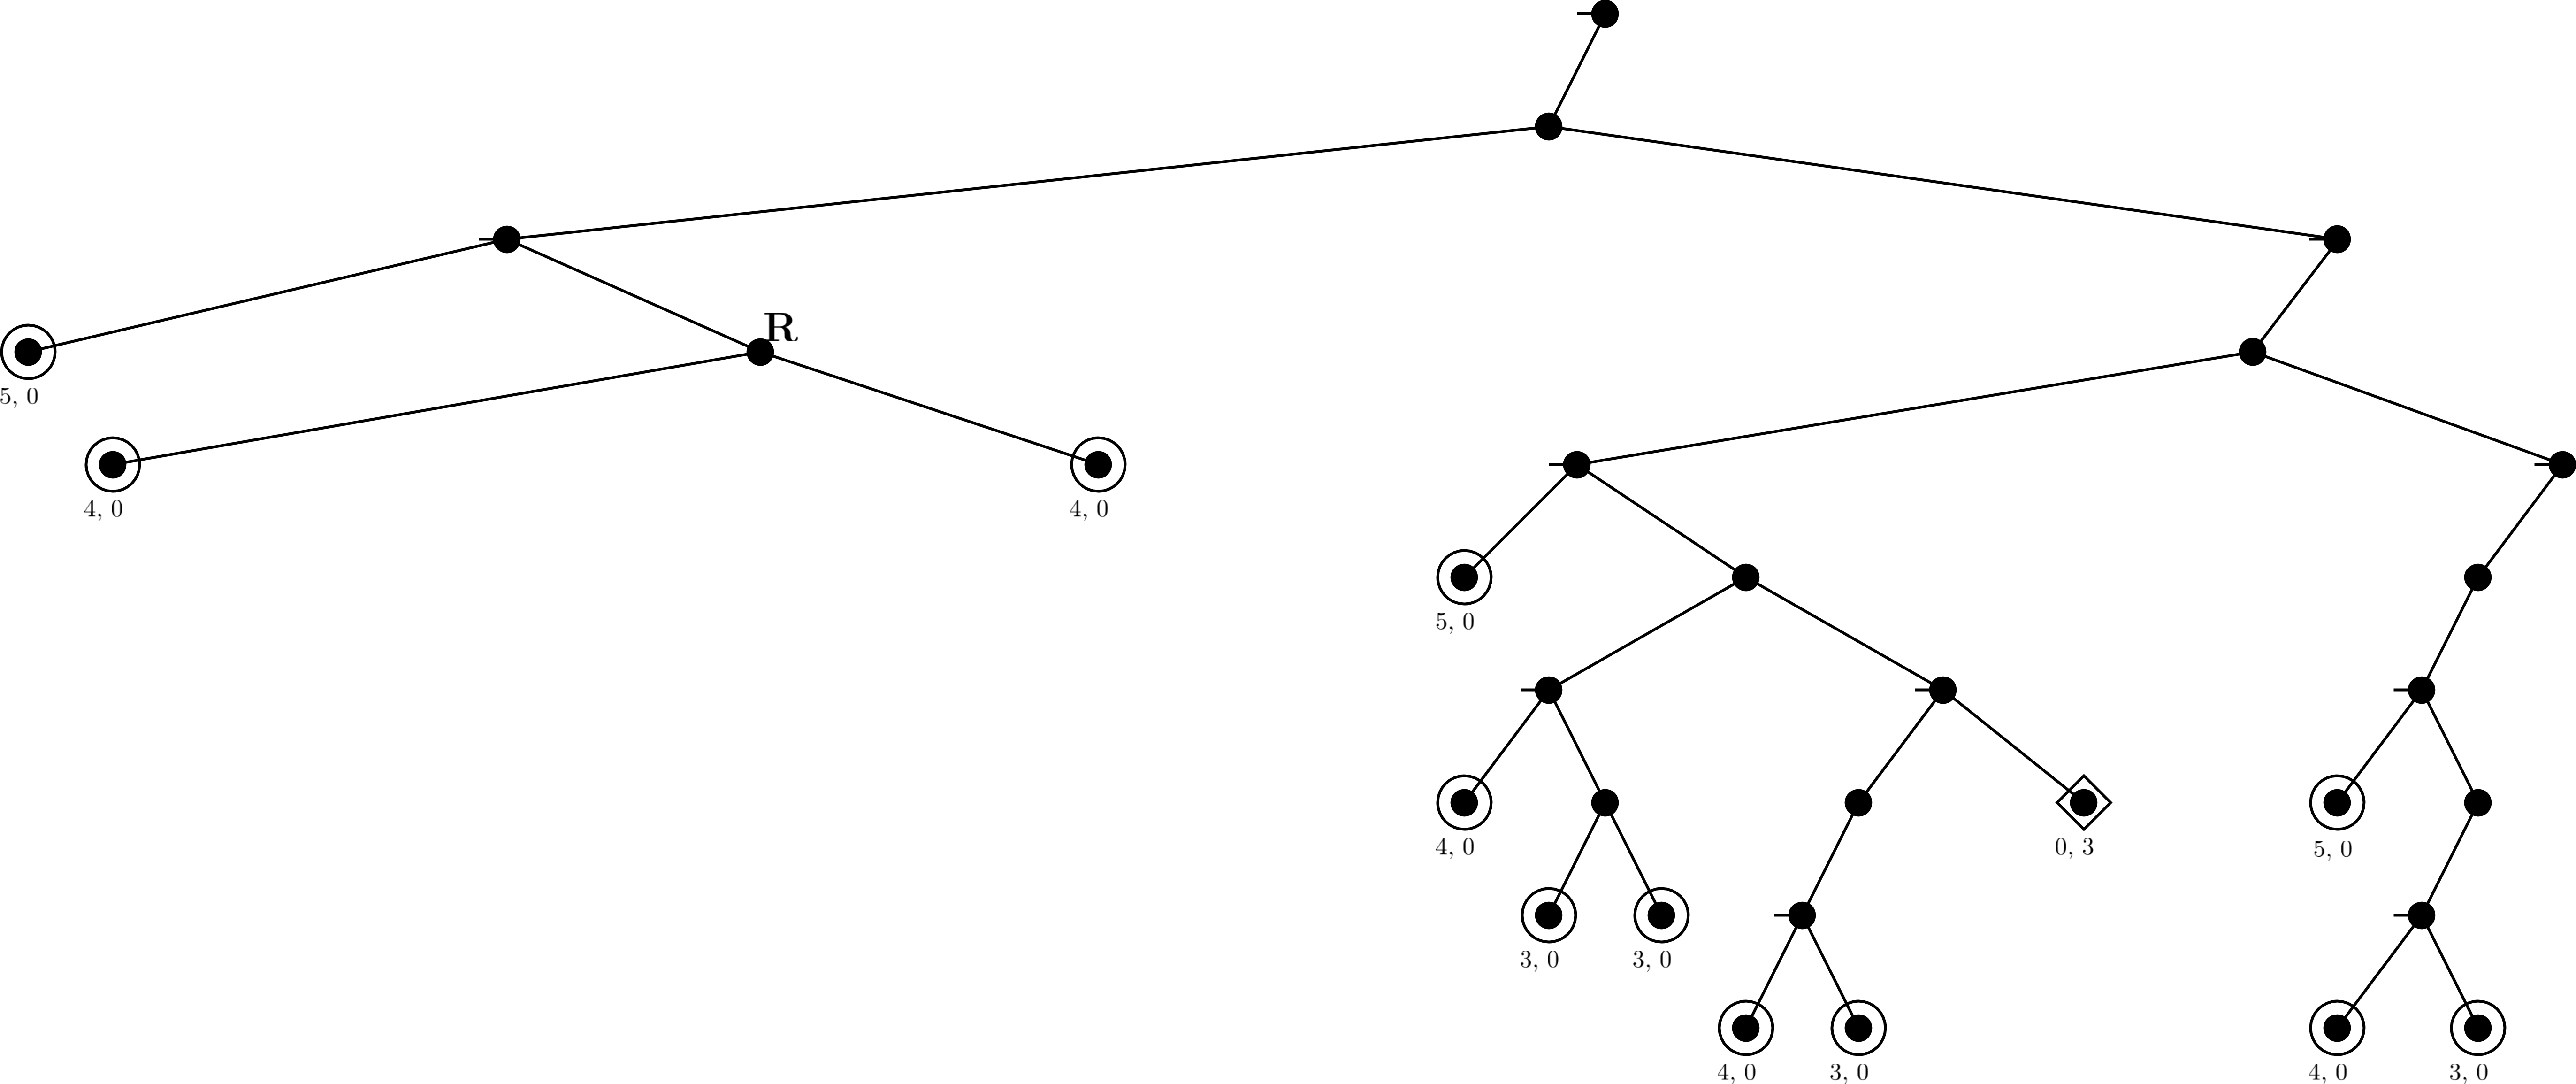
\includegraphics[width=13cm]{figures/Backwards5.png}
  \caption{The full game tree, after the subtrees are evaluated by the backwards induction algorithm in Figure \ref{fig:backwards2} and Figure \ref{fig:backwards4}.}
  \label{fig:backwards5}
\end{figure}
  
Now that most of the left side of the tree has been explored by the backwards induction algorithm, we return to view the full tree in Figure \ref{fig:backwards5}. The node $R$, a decision node for Player 2, must choose between two identical leaf nodes, both with (4, 0) utility. Thus, $R$ given a utility value of (4, 0). For the final decision on the left subtree, Player 1 chooses between a (5, 0) leaf node and a (4, 0) leaf node, and will select the former. Thus, the entire left subtree of is equivalent to a leaf node with utility (5, 0).

\begin{figure}[H]
  \centering
  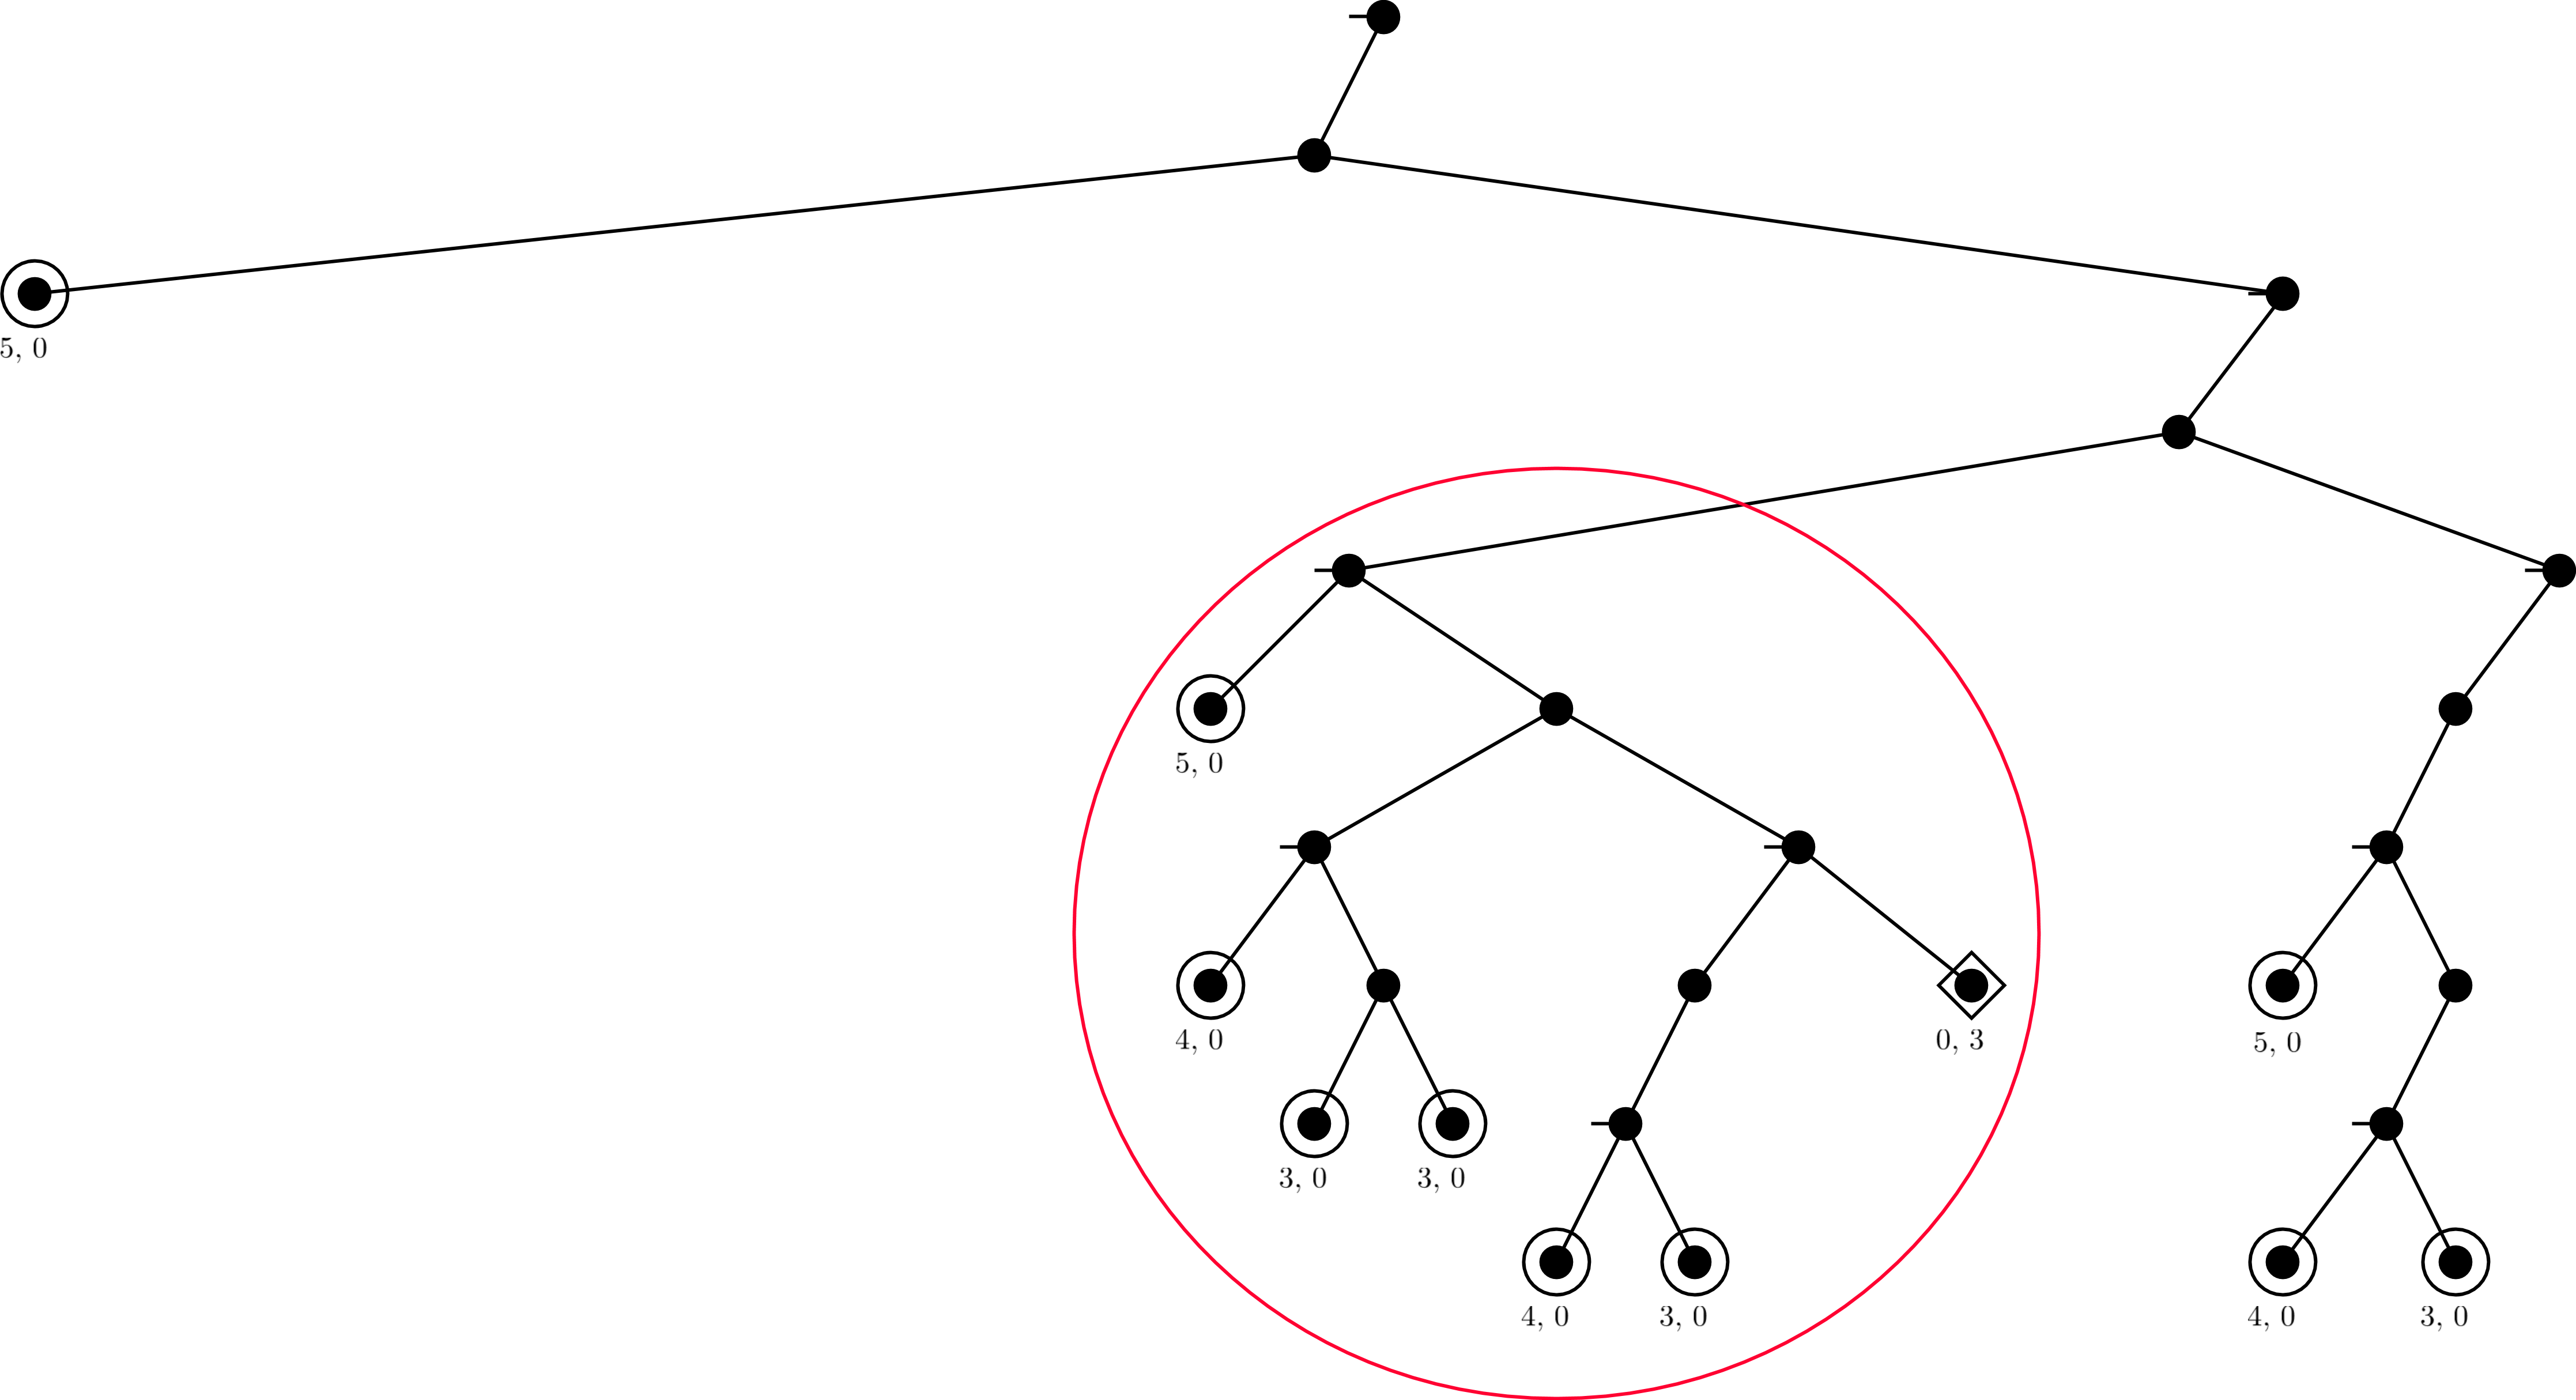
\includegraphics[width=13cm]{figures/Backwards6.png}
  \caption{The full game tree, after the backwards induction algorithm has recursed through half of the tree. The next subtree to be examined with the algorithm is circled in red.}
  \label{fig:backwards6}
\end{figure}

Now that the left subtree is reduced to a single leaf node, the algorithm moves to the right subtree and continues working. The next tree examined will be the circled subtree in Figure \ref{fig:backwards6}.\\

\begin{figure}[H]
  \centering
  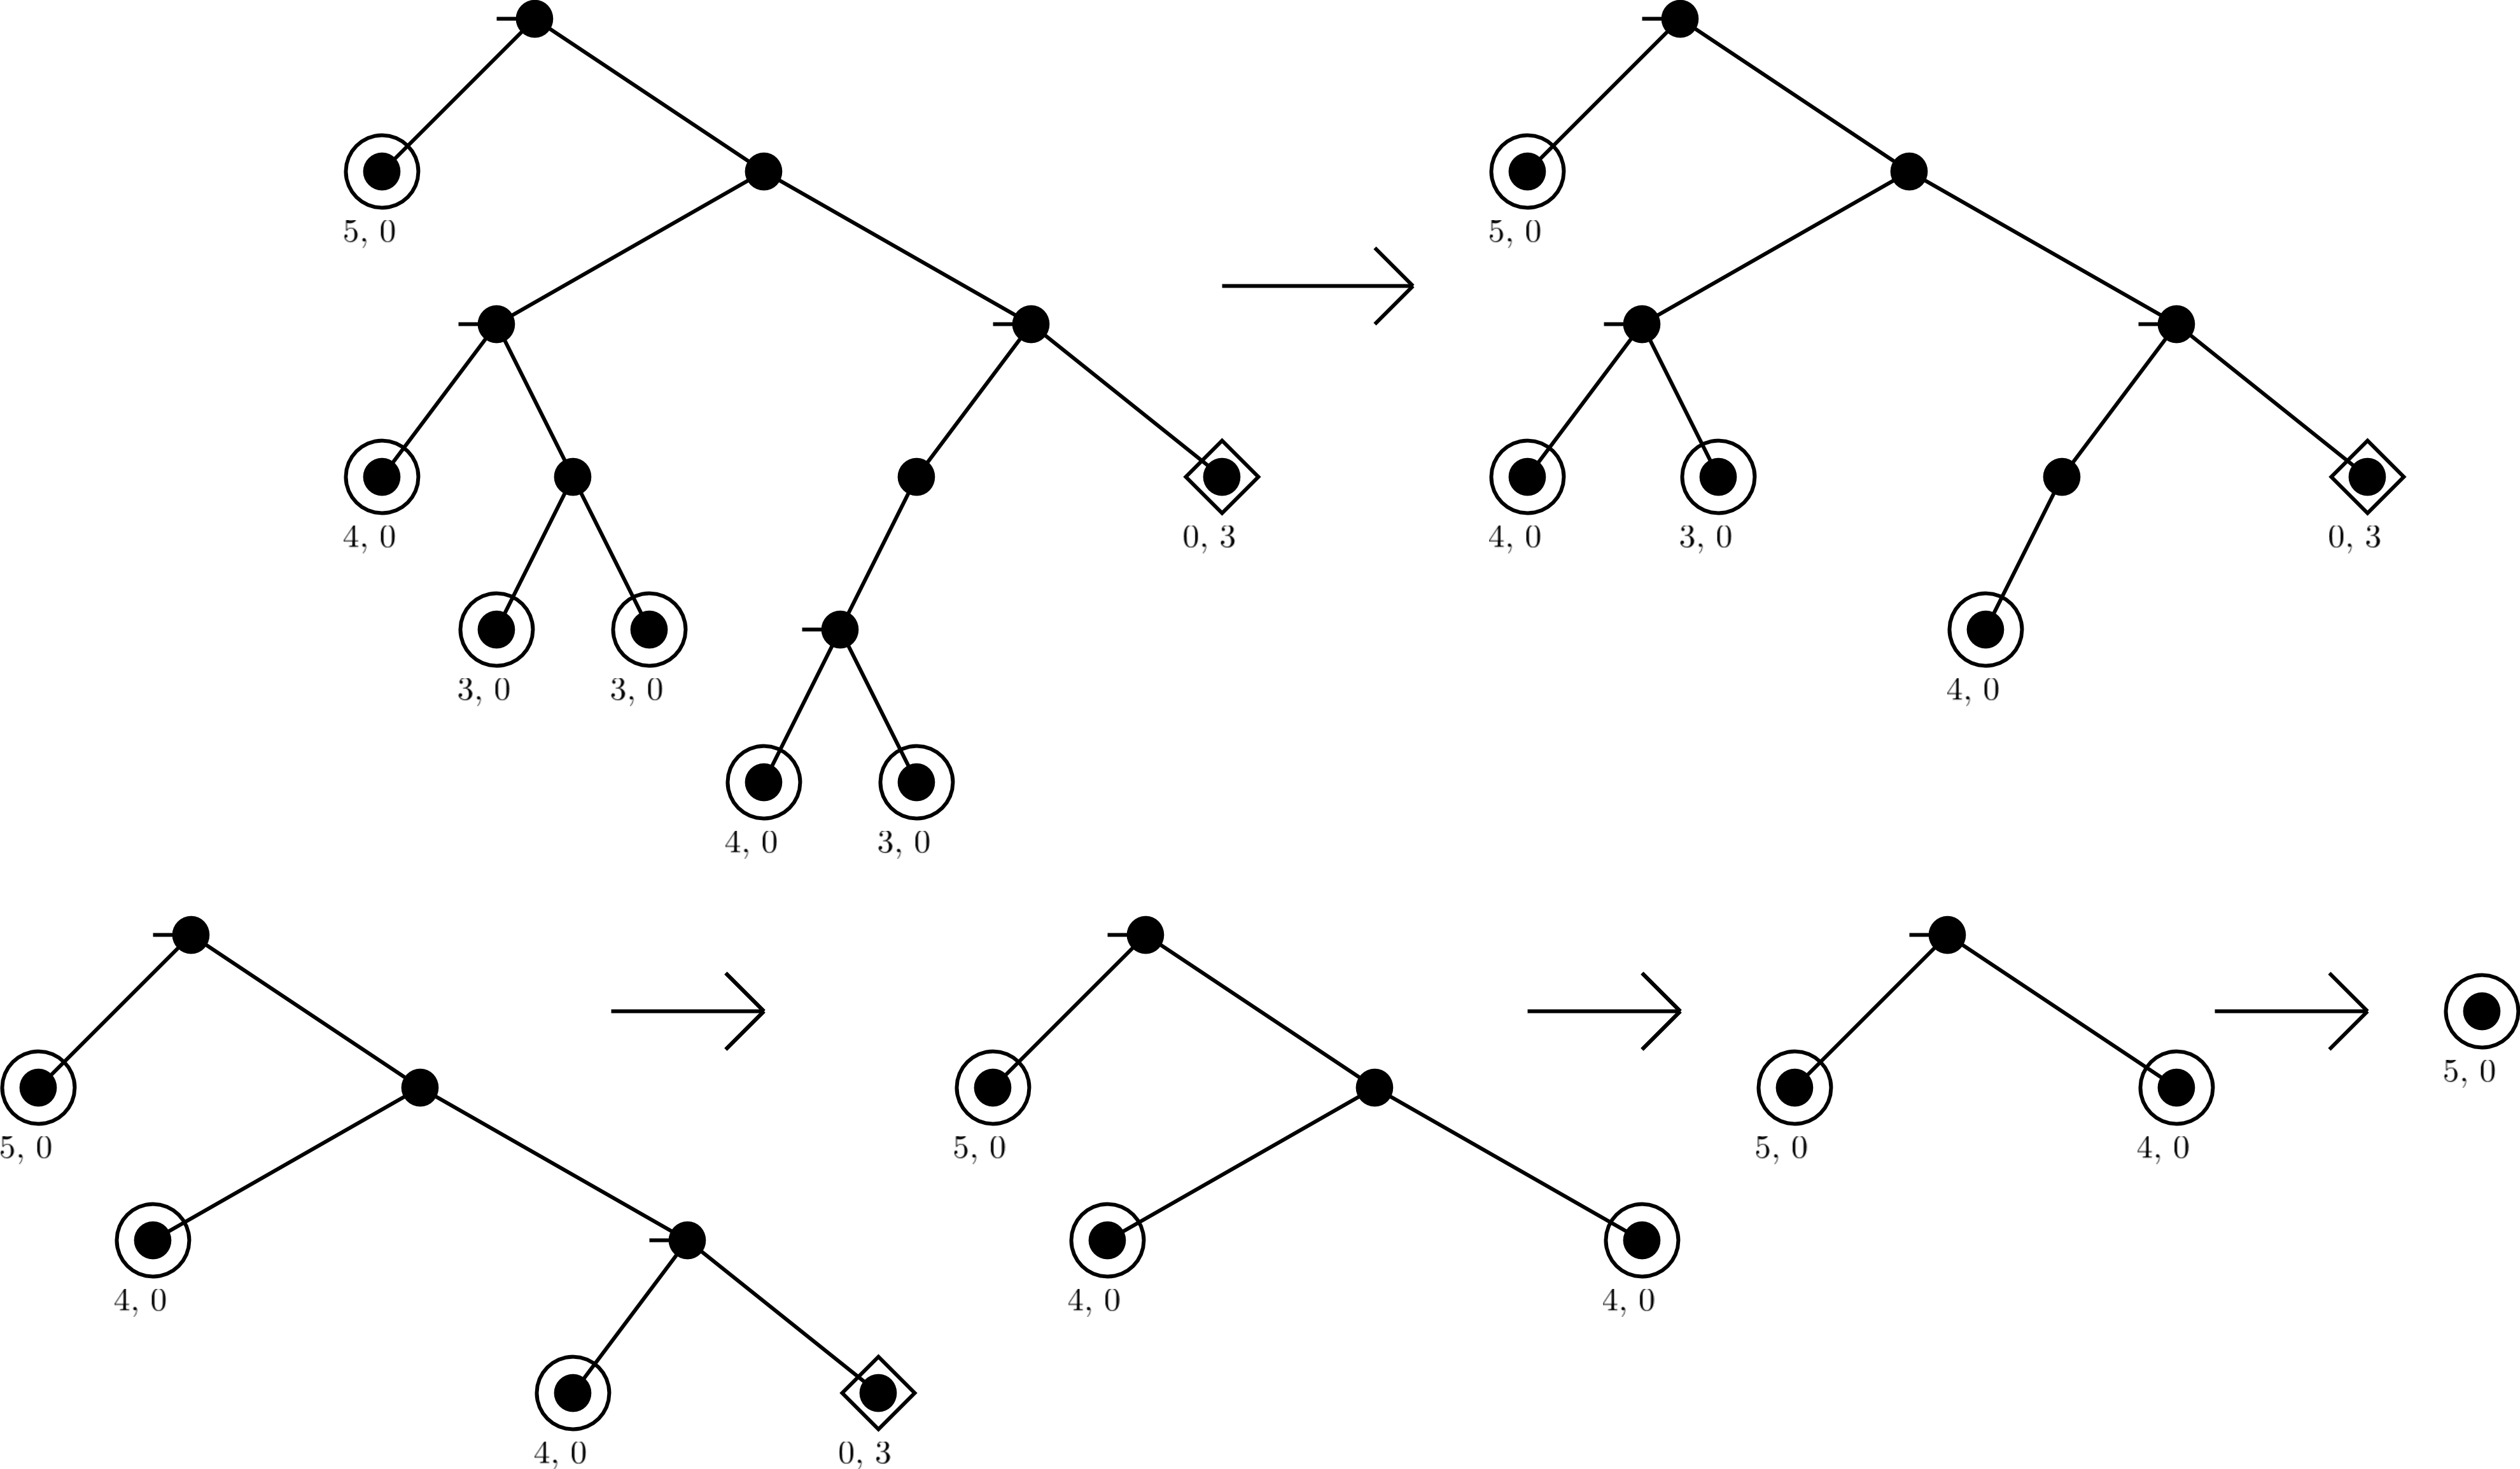
\includegraphics[width=12cm]{figures/Backwards7.png}
  \caption{The steps taken by the backwards induction algorithm after reaching the circled subtree in Figure \ref{fig:backwards6}.}
  \label{fig:backwards7}
\end{figure}

In the new subtree, the induction algorithm again determines which of the leaf nodes to bring up the tree. In the first step, at the lowest levels of the tree, player 1 makes a choice between (4, 0) and (3, 0), and player 2 makes a choice between (3, 0) and (3, 0). Player 1 chooses the former and player 2 chooses either. In the second step, player 1 chooses between (4, 0) and (3, 0) again, choosing the (4, 0) node again. In the third step, player 1 chooses between the (4, 0) and (0, 3) leaf nodes; player 1 will select the (4, 0) since they win at that node. In the next two steps, player 2 chooses between two equivalent (4, 0) nodes, then player 1 chooses between a (4, 0) node and a (5, 0) node. Thus, the subtree is equivalent to the (5, 0) leaf node.\\

\begin{figure}[H]
  \centering
  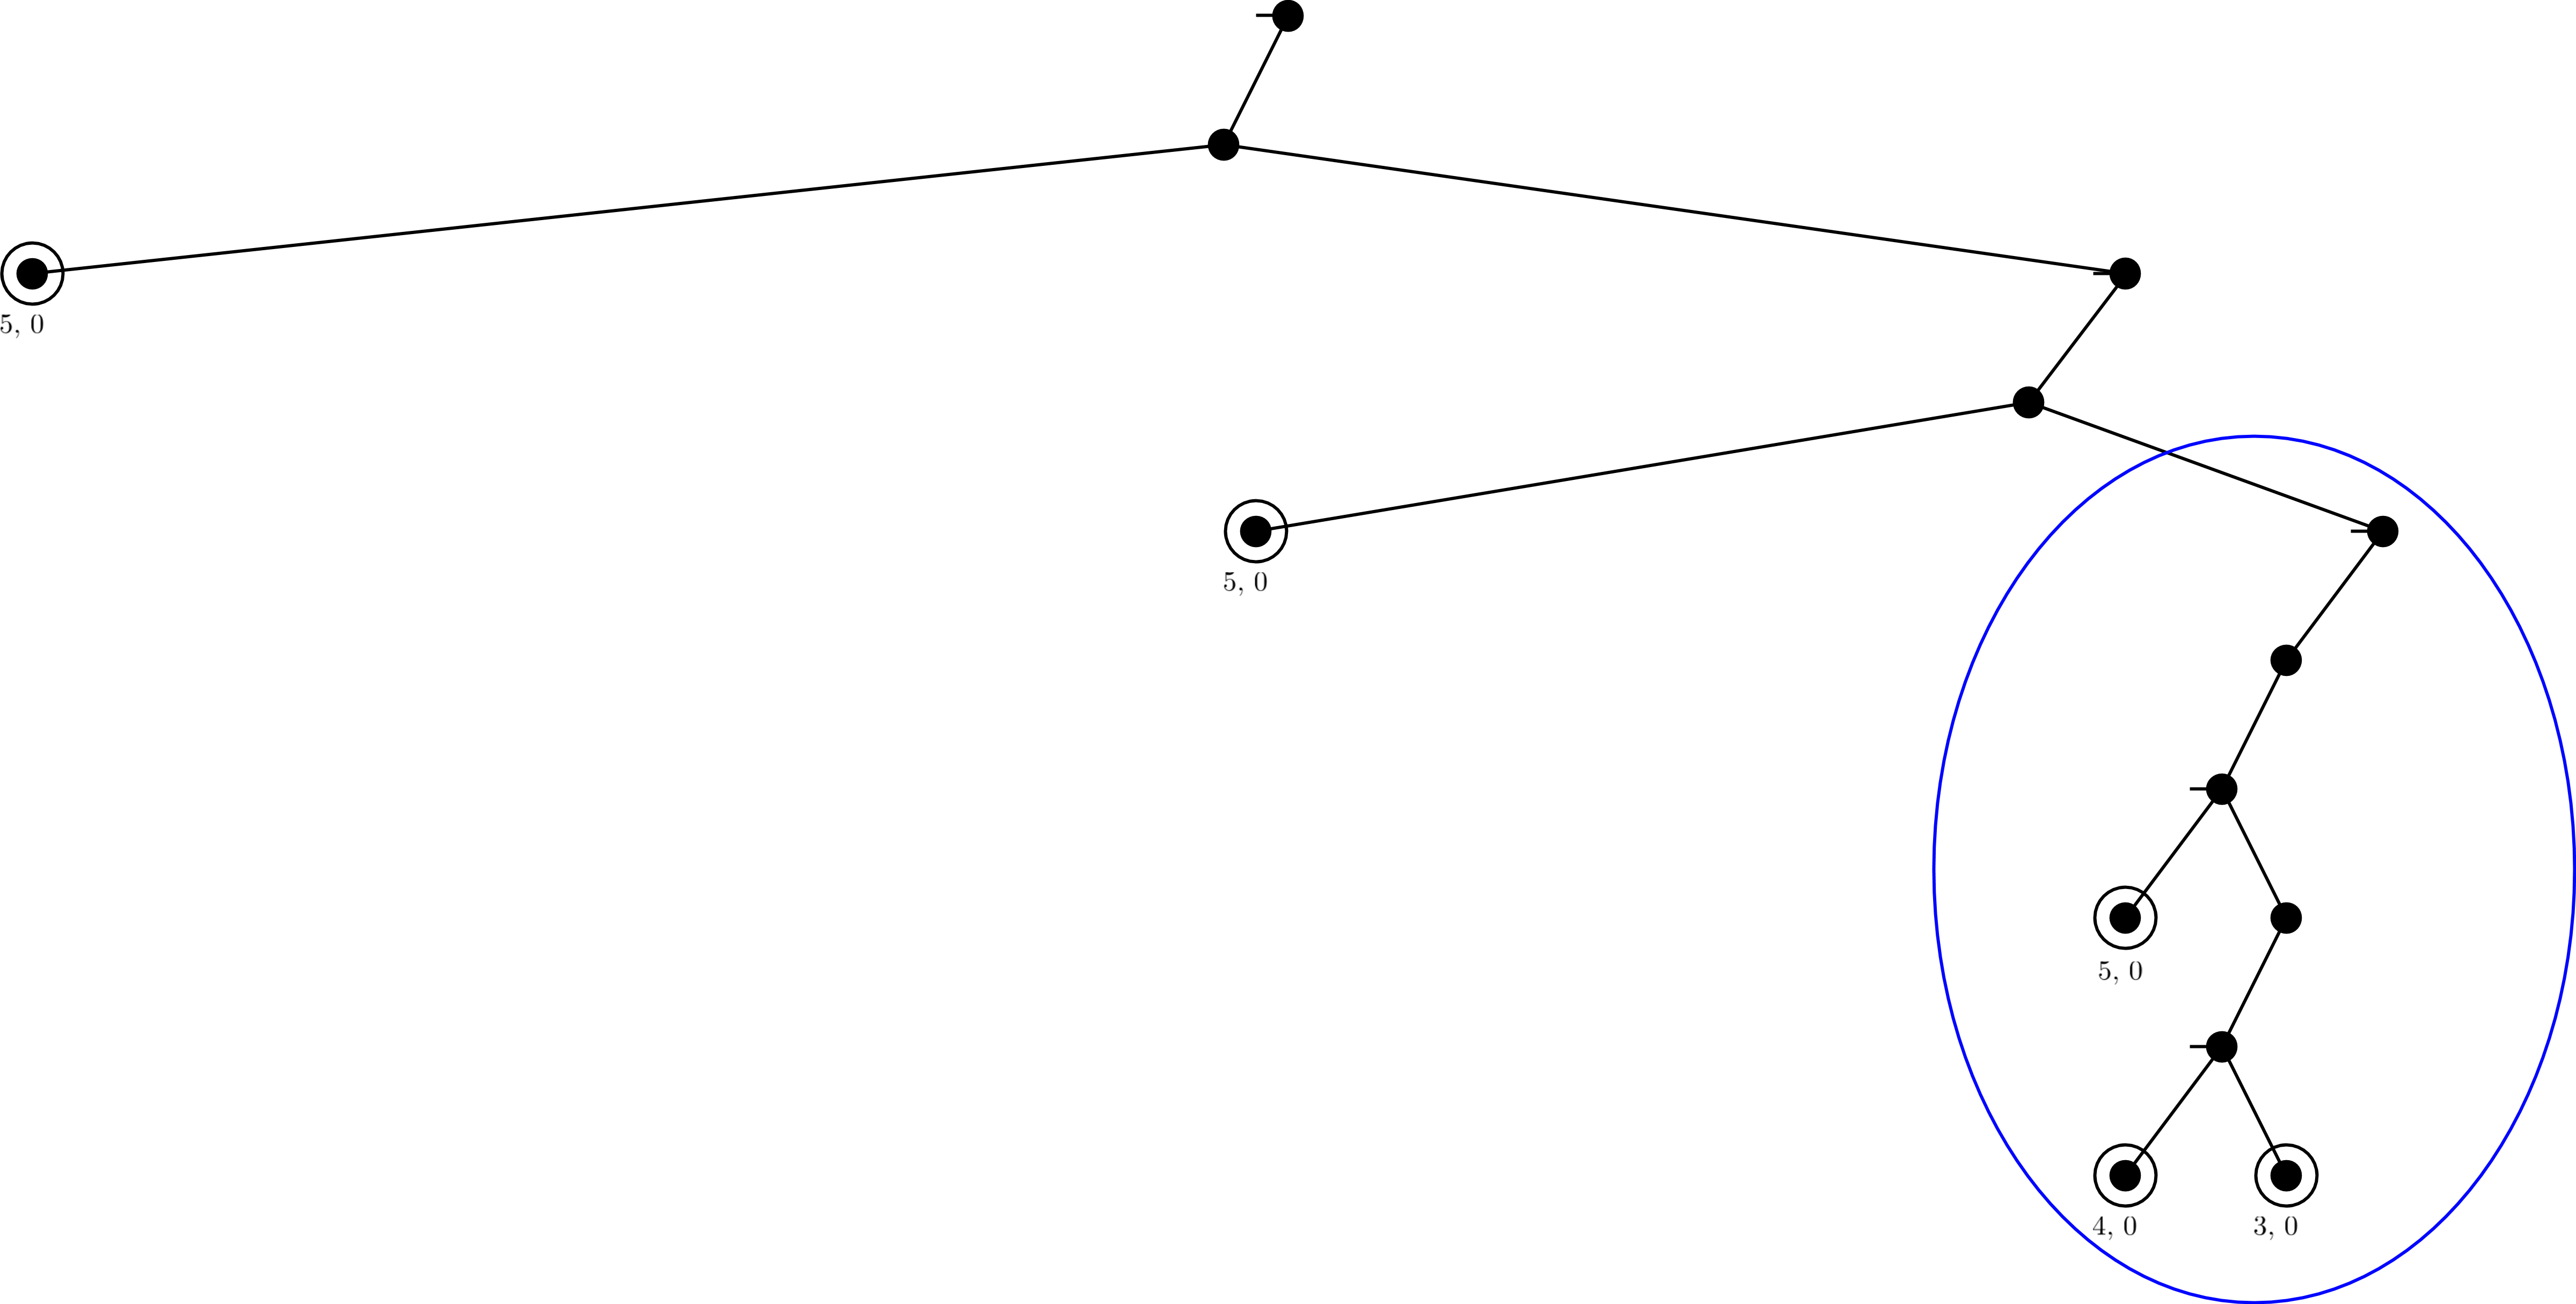
\includegraphics[width=14cm]{figures/Backwards8.png}
  \caption{The game tree in Figure \ref{fig:backwards6}, after the backwards induction steps performed in Figure \ref{fig:backwards7}. The blue circled subtree is the next to be evaluated by the algorithm.}
  \label{fig:backwards8}
\end{figure}

With the subtree in Figure \ref{fig:backwards7} evaluated, the subtree is replaced with the leaf node (5, 0) as shown in Figure \ref{fig:backwards8}. Next, the algorithm will perform the same analysis on the subtree circled in blue.

\begin{figure}[H]
  \centering
  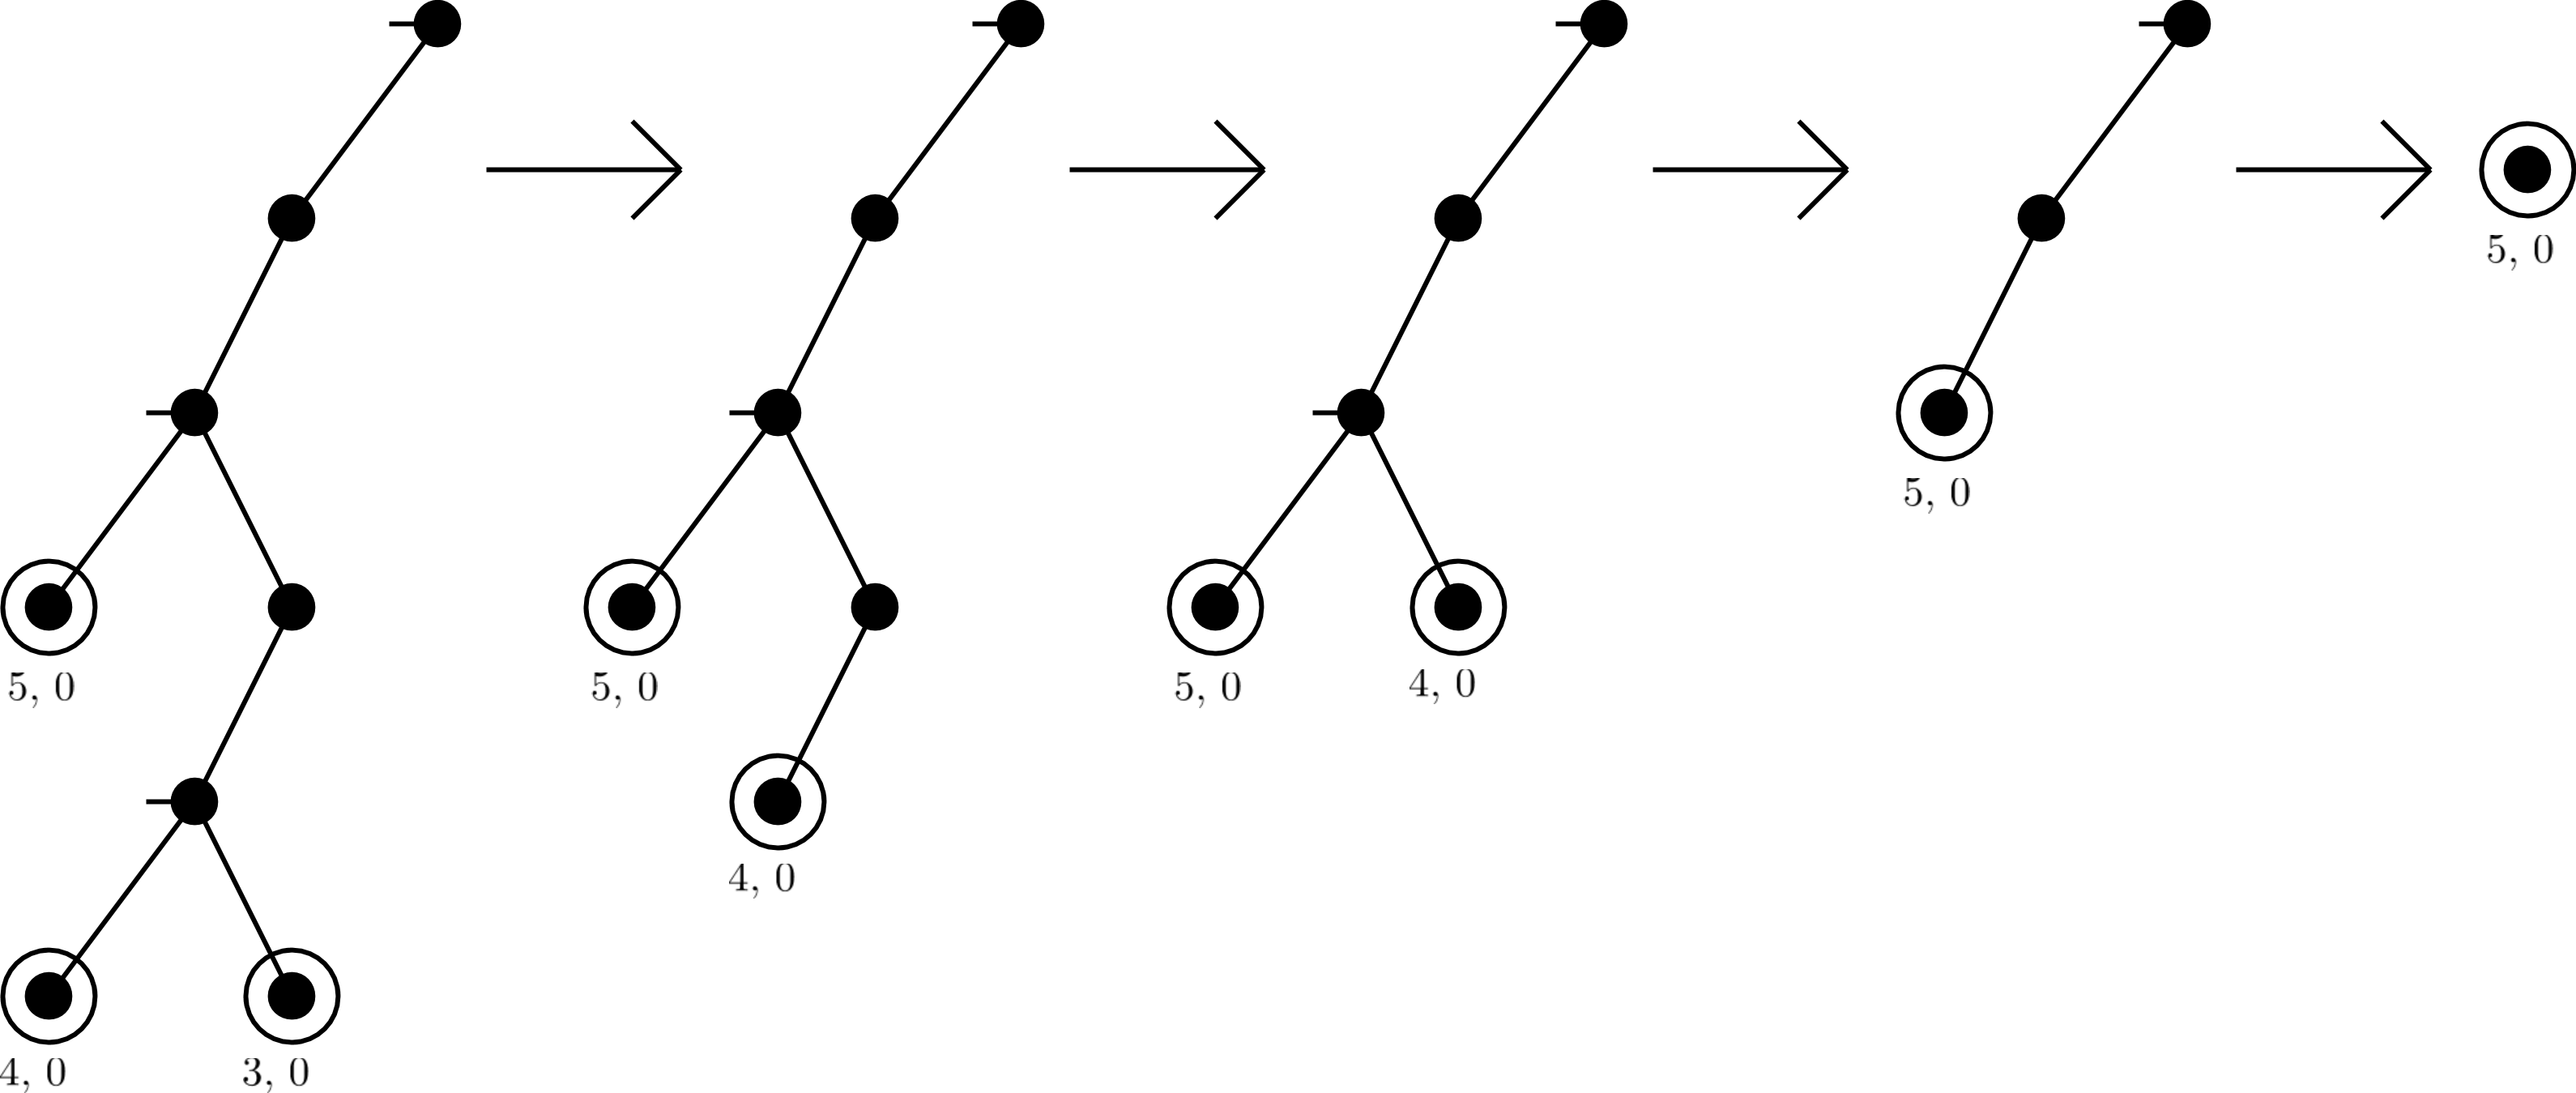
\includegraphics[width=11cm]{figures/Backwards9.png}
  \caption{The steps taken by the backwards induction algorithm after reaching the circled subtree in Figure \ref{fig:backwards8}.}
  \label{fig:backwards9}
\end{figure}

For this final subtree in Figure \ref{fig:backwards9}, player 1 first makes a choice between the (4, 0) and (3, 0) leaf nodes at the bottom of the tree and picks the former. Since player 2 only has one choice at their decision node, the (4, 0) node is brought up one level more. Player 1 makes a second choice between (4, 0) and (5, 0), choosing the latter. There are no more decisions on this section of the tree, so the subtree is equivalent to a leaf node with utility (5, 0).

\begin{figure}[H]
  \centering
  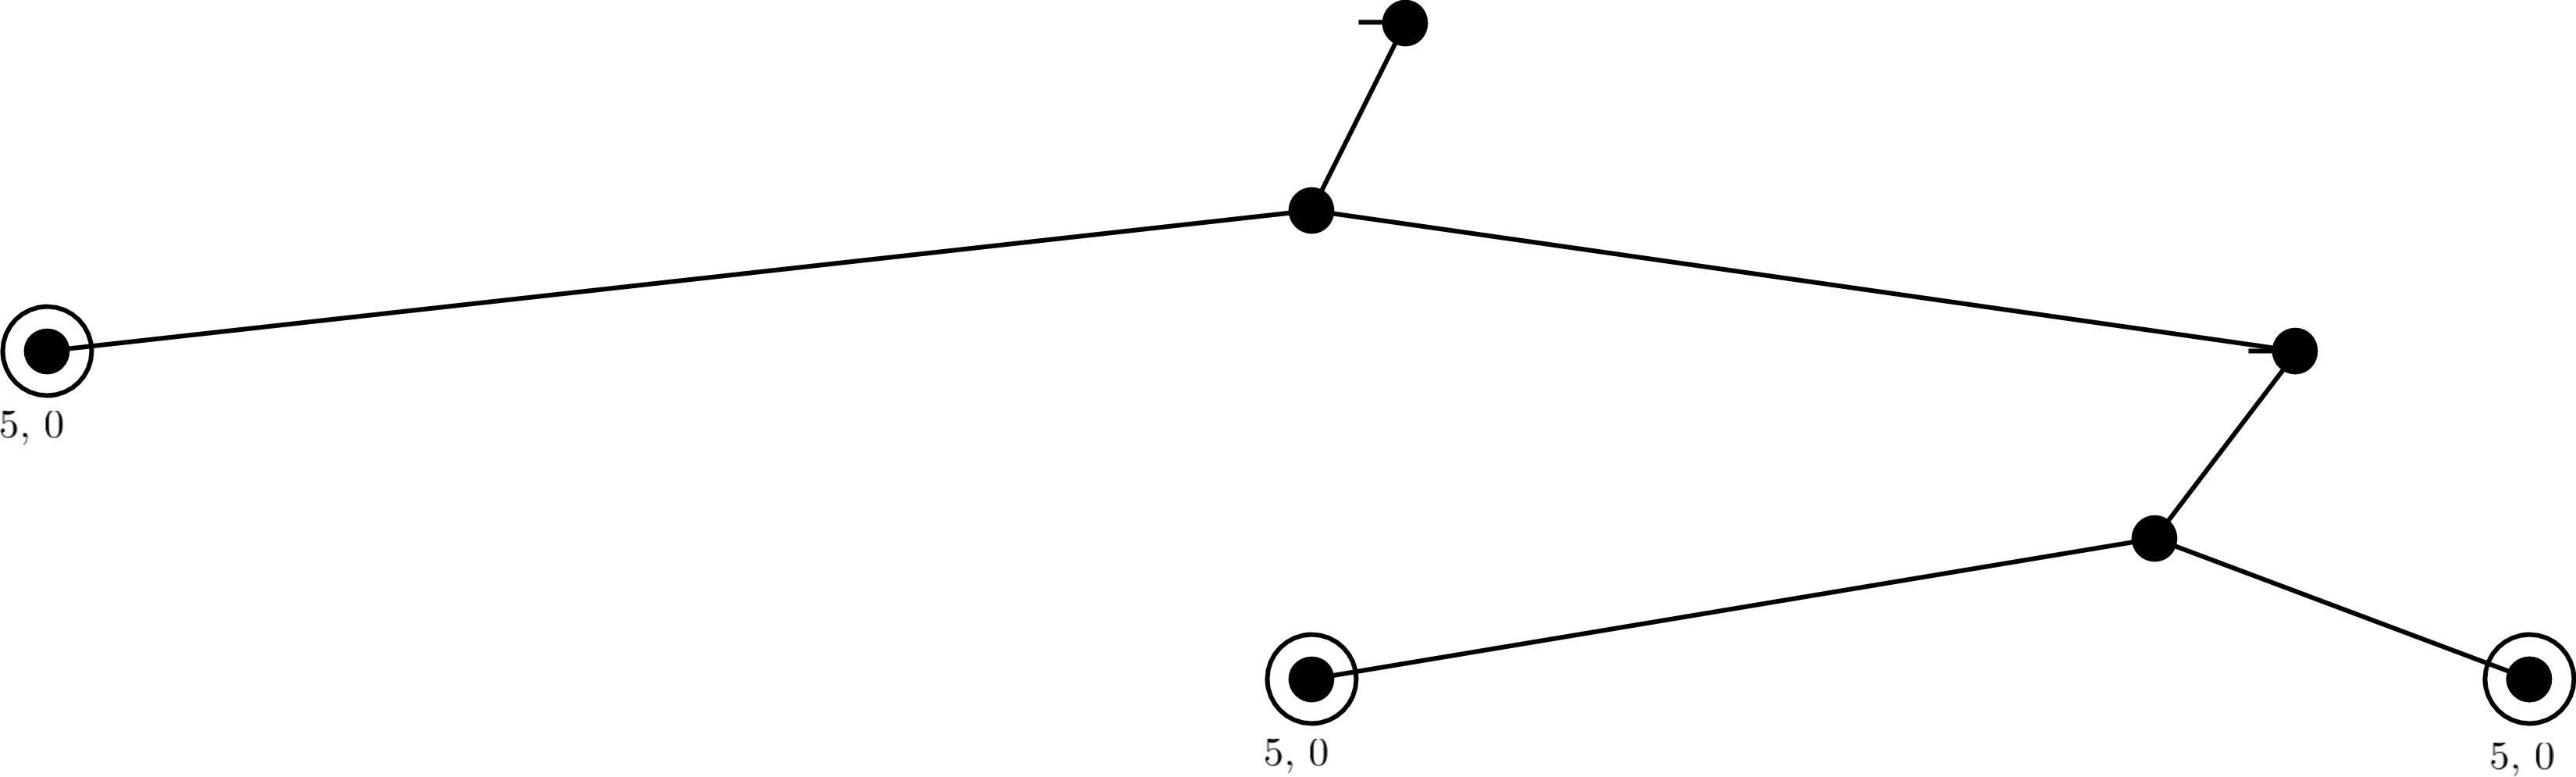
\includegraphics[width=12cm]{figures/Backwards10.png}
  \caption{The game tree in Figure \ref{fig:backwards8}, after the backwards induction steps performed in Figure \ref{fig:backwards9}. At this point, all leaf nodes have equal utility, so the entire tree is equivalent to the single leaf node with utility (5, 0).}
  \label{fig:backwards10}
\end{figure}

After the steps taken in Figure \ref{fig:backwards9}, the tree for the entire game is equivalent to the tree in Figure \ref{fig:backwards10}. At this stage, all the leaf nodes have the same utility value: (5, 0). Thus, no matter which player is making the decision, any choice they make in this tree will lead to an outcome of (5, 0). If both players are making optimal decisions, the outcome of a game in Figure \ref{fig:backwards10} will therefore always be (5, 0).

\subsubsection{Analysis}
Player 1 has a huge advantage in this game by taking the first action. If both players only choose to attack, then Player 1 wins the game. The utility of this outcome is (5, 0), and is thus one of the optimal strategies for the game, as established. In fact, Player 1 can only lose by choosing to heal at certain points in the game.\\

In all four paths where Player 2 won, there is a node where Player 1 chose to heal from 9 HP to 10 HP. If Player 1 only attacks, then Player 2 has no chance of victory. Since the normal amount of HP recovered by healing is 4 HP, we can see that Player 1 is wasting potential HP by using one of their turns to heal when their HP is already close to the HP cap. We may infer that, in games with larger HP caps, the same effects would appear. It is much more useful for a player to heal when their HP is closer to zero.\\

In this limited model, it is clear that healing is not a viable strategy. Since players can only attack or heal, one player's choice to heal will either have no effect on their utility or a negative effect on their utility. If Player 2 heals and Player 1 immediately attacks, then Player 2 has a net loss of 1 HP. The HP recovered by a player is not enough to offset the damage dealt by their opponent. If a player heals and their opponent also heals, then the difference in utility is zero. Situations where both players heal at the same time does not change the overall performance of the players. If Player 2 was losing to Player 1, and both players heal, then Player 2 will still be losing to Player 1. At the most, choosing to heal only delays the inevitable.\\

Now that some patterns in the game are identified, we expand the choices of the game and build a prototype using Python and the pygame library.

\section{Game Engine}
Python was chosen as the development language for this game. Python is an extremely portable language: anyone with Python installed can run the code. Python also has a robust library for two-dimensional games called pygame, which was essential in creating this game. Specifically, Python 3 was used for better compatibility with the pygame library and for the \texttt{copy()} function for arrays.

\subsection{The pygame Library}
The pygame library provides a number of Python functions that are useful in creating a two-dimensional video game. The library was originally created in 2001 to combine Python with SDL (Simple DirectMedia Layer), a library of multimedia controls written for C \cite{shinners}. pygame can utilize a variety of different graphics libraries, including OpenGL, DirectX, the Linux frame buffer, and an ASCII art backend \cite{shinners}. The pygame library is supported by numerous operating systems, and the core functions of pygame use highly optimized C or assembly code.\\

At the top level, pygame controls the initialization and exiting of its various modules, particularly the \texttt{pygame.display} module which renders the game. pygame features two functions to update a display window, \texttt{pygame.display.flip()} and \texttt{pygame.display.update()}. \texttt{display.flip()} works with two separate arrays, containing the pixel data for the window in which the game operates. One array is displayed on the screen, while the other array is used to record changes made to the on-screen image. Once all changes are made, \texttt{display.flip()} swaps these arrays, or ``buffers,'' by copying all the data from one array into the other. The buffer that recorded changes is now displayed on-screen, while the buffer that was displayed can now be used to record further changes. \texttt{display.update()} is an optimized version of \texttt{flip()} that takes as an argument a rectangle or a sequence of rectangles. These rectangles correspond to the areas of the display that need to be updated. For instance, passing the coordinates of a rectangle over a game's scoreboard only updates the scoreboard. With this function, large sections of the pixel array do not need to be copied from one buffer to another, speeding up the rendering process.\\

The two main objects in pygame are the \texttt{Surface} object and the \texttt{sprite} object. Surfaces can be changed with pygame to alter various attributes. For instance, the \texttt{alpha} value, or the transparency of the surface, can be changed with \texttt{set\_alpha()}. The individual color values can be converted to integers and vice versa with the \texttt{map\_rgb()} and \texttt{unmap\_rgb()} functions, respectively. This allows for pygame to store colors as a single number, rather than a tuple of integers. Surfaces are mostly used to load image files and to create backgrounds for the game. Sprites, on the other hand, are used for the actual in-game objects, such as enemies, player characters, and projectiles. Sprites can be stored in a \texttt{Group} object, that can be used to separate sprites by different purposes. Each sprite draws its image to a \texttt{Surface}, provided that it has a \texttt{Surface.image} and \texttt{Surface.rect} attribute.\\

Once a sprite or surface is created with an image, pygame can also perform graphical transformations on that image. The \texttt{pygame.transform} module has functions to flip, rotate, and scale an image. Another pygame feature is the ability to do collision detection on sprites and rectangles.\\

For the actual gameplay of a pygame program, there are also modules for joystick, mouse, and keyboard controls. A sound mixer module allows audio tracks to be played in the game, and the \texttt{pygame.time} module can be used to control the framerate of the game.
\newpage
\subsection{Gameplay Design}
For the expanded version of the game, several things were changed from the game in Figure \ref{fig:gameTree}. Two additional choices were added: Parry and Strong Attack. With Parry, the player enters a guarded stance until their next turn; this player will be referred to as the defending player. If, before their next turn, their opponent attacks them, the defending player counter-attacks. The defending player loses no HP, and the player who attacked them loses 3 HP from the counter-attack. A Strong Attack does more damage than a regular attack (7 HP vs 5 HP), but has a chance to miss the opponent completely and do no damage. Additionally, a Strong Attack is unaffected by Parry; if a player is Parrying and their opponent uses a strong attack, the parry is unsuccessful and the defending player suffers 7 HP of damage.

\lstset{language=python, label=lst:aiClass, caption={The \texttt{PlayerAvatar} class and its helper function, \texttt{helperAIFunc()}.}}
\begin{lstlisting}
class PlayerAvatar:
  def __init__(self, model):
    self.hp = 25
    self.maxHP = 25
    self.healTurns = 2
    self.isParrying = False
    self.aggressiveness = .25
    self.AI_MODEL = model
# AI Helper Function - Picks the appropriate function to call, and passes the correct
# information
  def helperAIFunc(self, enemyHP, isParrying):
    if self.AI_MODEL == 1:
      return self.randomAI()
    elif self.AI_MODEL == 2:
      return self.aggressiveRandomAI()
    elif self.AI_MODEL == 3:
      return self.fiftyPercentAI()
    elif self.AI_MODEL == 4:
      return self.comparativeAI(enemyHP)
    elif self.AI_MODEL == 5:
      return self.scalingDifficulty(enemyHP)
    elif self.AI_MODEL == 6:
      return "A"
    elif self.AI_MODEL == 7:
      return self.parryCountering(enemyHP, isParrying)
    else:
      return self.limitedRandomAI()
\end{lstlisting}

The two players in the game begin with 25 HP each, and are able to heal twice per game. These values are stored in a \texttt{PlayerAvatar} class, as shown in Listing \ref{lst:aiClass} at lines 3-5. This class also stores the type of AI used for the computer player, at line 8. The class has a helper function, \texttt{helperAIFunc}, which is called from within the main game loop. In this helper function, the class variable \texttt{self.AI\_MODEL} is used in a series of \texttt{if} statements to call that model's respective function. Notice that the \texttt{elif} statement at line 22 does not call a function, but instead returns the character ``A.'' This corresponds to the baseline AI model, assigned to the Beserker character; this model and all the other AI functions will be discussed later in this section. Each of the AI functions in the helper function return one of four characters: ``A,'' ``S,'' ``P,'' or ``H.'' These correspond to the four possible actions in the game: Attack, Strong Attack, Parry, and Heal. These characters are returned to the main game loop, which adjusts the game based on the action taken.\\

Eight different AI models were created. In all models, the AI checks to see if any healing turns remain; if not, the AI chooses a different option. The specific replacement action varies from one model to another. Three of the models rely on a random number generator to make their decisions.\\

\begin{figure}[H]
  \centering
  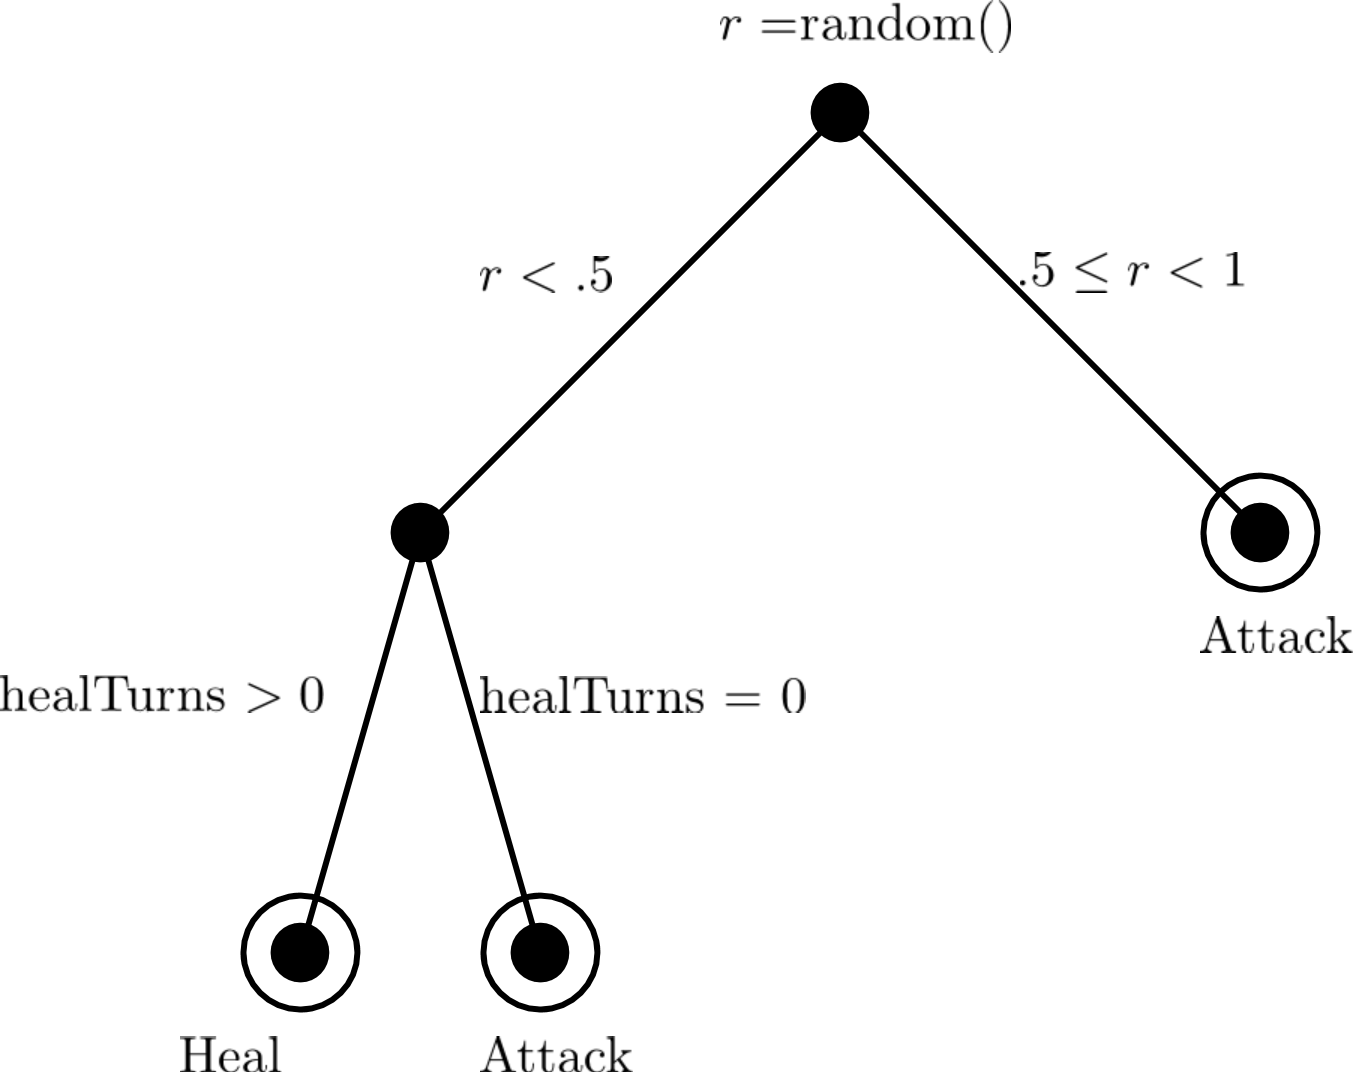
\includegraphics[width=6cm]{figures/AILimitedRandom.png}
  \caption{The decision tree for the \texttt{limitedRandomAI()} function.}
  \label{fig:AI1}
\end{figure}

The first AI model, the \texttt{limitedRandomAI()} function, chooses randomly to attack or heal with a 50/50 chance of either, but will use a normal attack instead if the AI has already healed itself twice. This is shown by the decision tree in Figure \ref{fig:AI1}. The variable $r$ is given a random value between 0 and 1, and the first decision in the tree is based on the value of $r$. After that, the tree has either reached a leaf node (for $r\ge .5$) or must make a second decision, this time based on the number of healing turns remaining. Given the limited success Player 2 had in the original game tree in Figure \ref{fig:gameTree}, this model was not used in the final version of the game. Instead, a different model was used which could perform all four possible actions.\\

\begin{figure}[H]
  \centering
  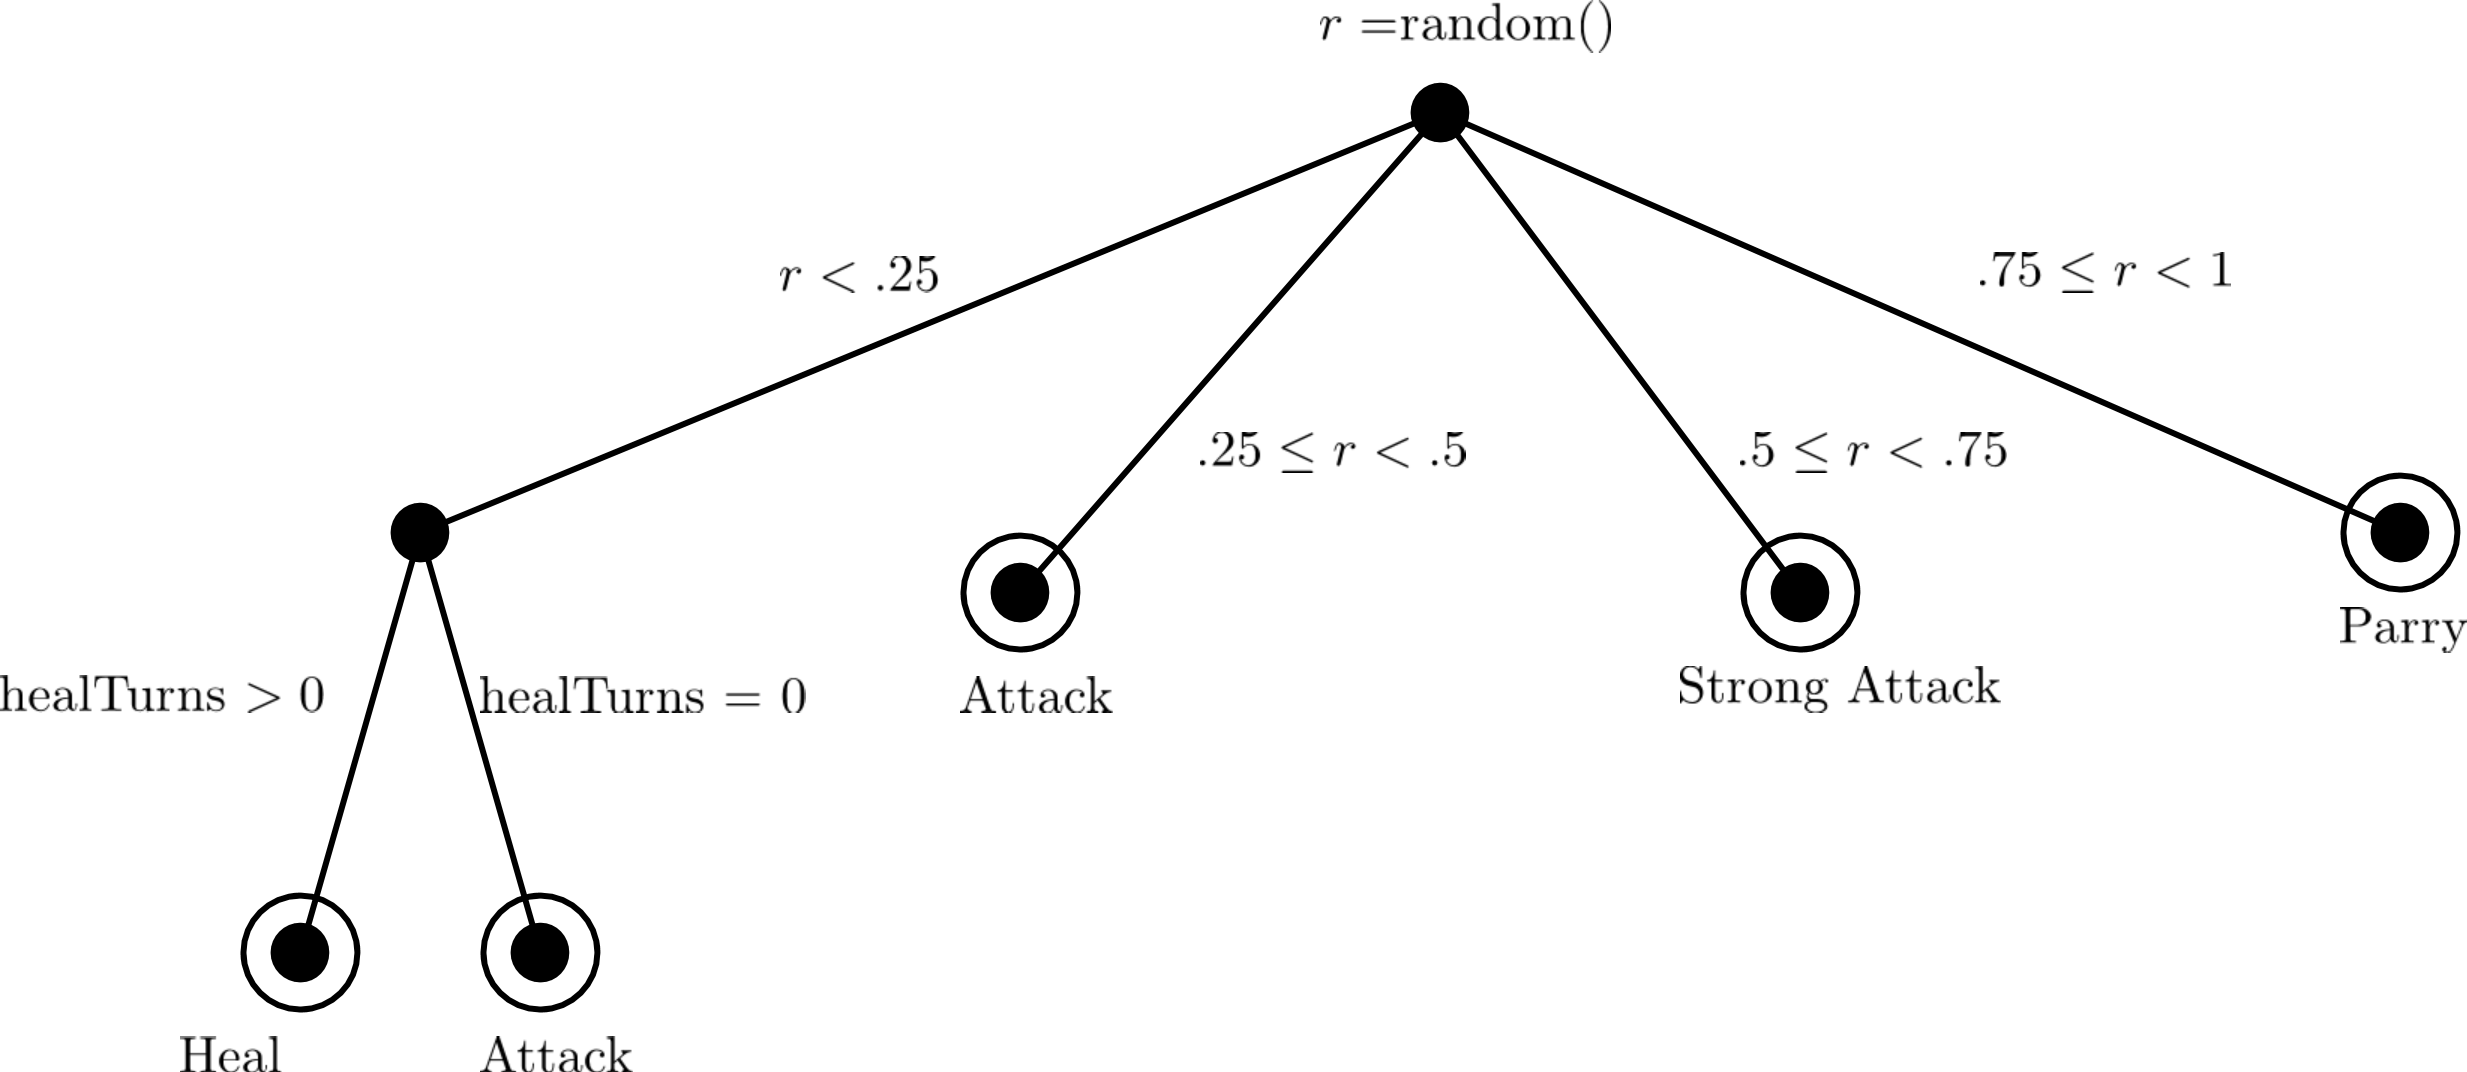
\includegraphics[width=10cm]{figures/AIRandom.png}
  \caption{The decision tree for the \texttt{randomAI()} function.}
  \label{fig:AI2}
\end{figure}
The second model, \texttt{randomAI()}, has a 25\% chance of attacking, healing, parrying, or using a strong attack. Again, Figure \ref{fig:AI2} shows that if the random number generator chooses to heal, but all healing turns have been used, the AI does a normal attack instead. This choice was made to affect a sense of desperation in the AI: when an opponent no longer can heal themselves, they become more offensive to try and win the battle. This kind of behavior - where the AI changes their strategy after all healing turns have been spent - is incorporated into all the models.\\

\lstset{language=python, label=lst:randomAI, caption={The \texttt{randomAI()} function.}}
\begin{lstlisting}
# AI Model 2 - Randomly choose between 4 actions: Attack, Strong Attack, Parry, and Heal.
# If no heal turns remain, the AI does a normal attack
def randomAI(self):
  newAction = ""
  r=random()
  if(r<.25 and self.healTurns > 0):
    newAction = "H"
  elif(r<.5):
    newAction = "A"
  elif(r<.75):
    newAction = "S"
  else:
    newAction = "P"
  return newAction
\end{lstlisting}

Listing \ref{lst:randomAI} shows the code used to create the decision tree in Figure \ref{fig:AI2}. In the code, each range of values is compared to the random variable $r$ - Python's \texttt{random()} function returns a number in the range $[0, 1)$ - and the action is determined by the range into which $r$ falls. Since Python executes each line of code sequentially, lower bounds on the ranges are not needed; the lower bounds are implicit from the previous \texttt{if} or \texttt{elif} statements. In comparison with the tree, the program condenses the two Attack nodes together with the first \texttt{elif} clause. Since the first \texttt{if} statement checks for both \texttt{r<.25} and \texttt{self.healTurns>0}, the two branches of the decision tree leading to the Heal leaf node are both covered. This format cannot be done directly with decision trees, since each decision node in the tree must use a single variable to split its branches.

\begin{figure}[H]
  \centering
  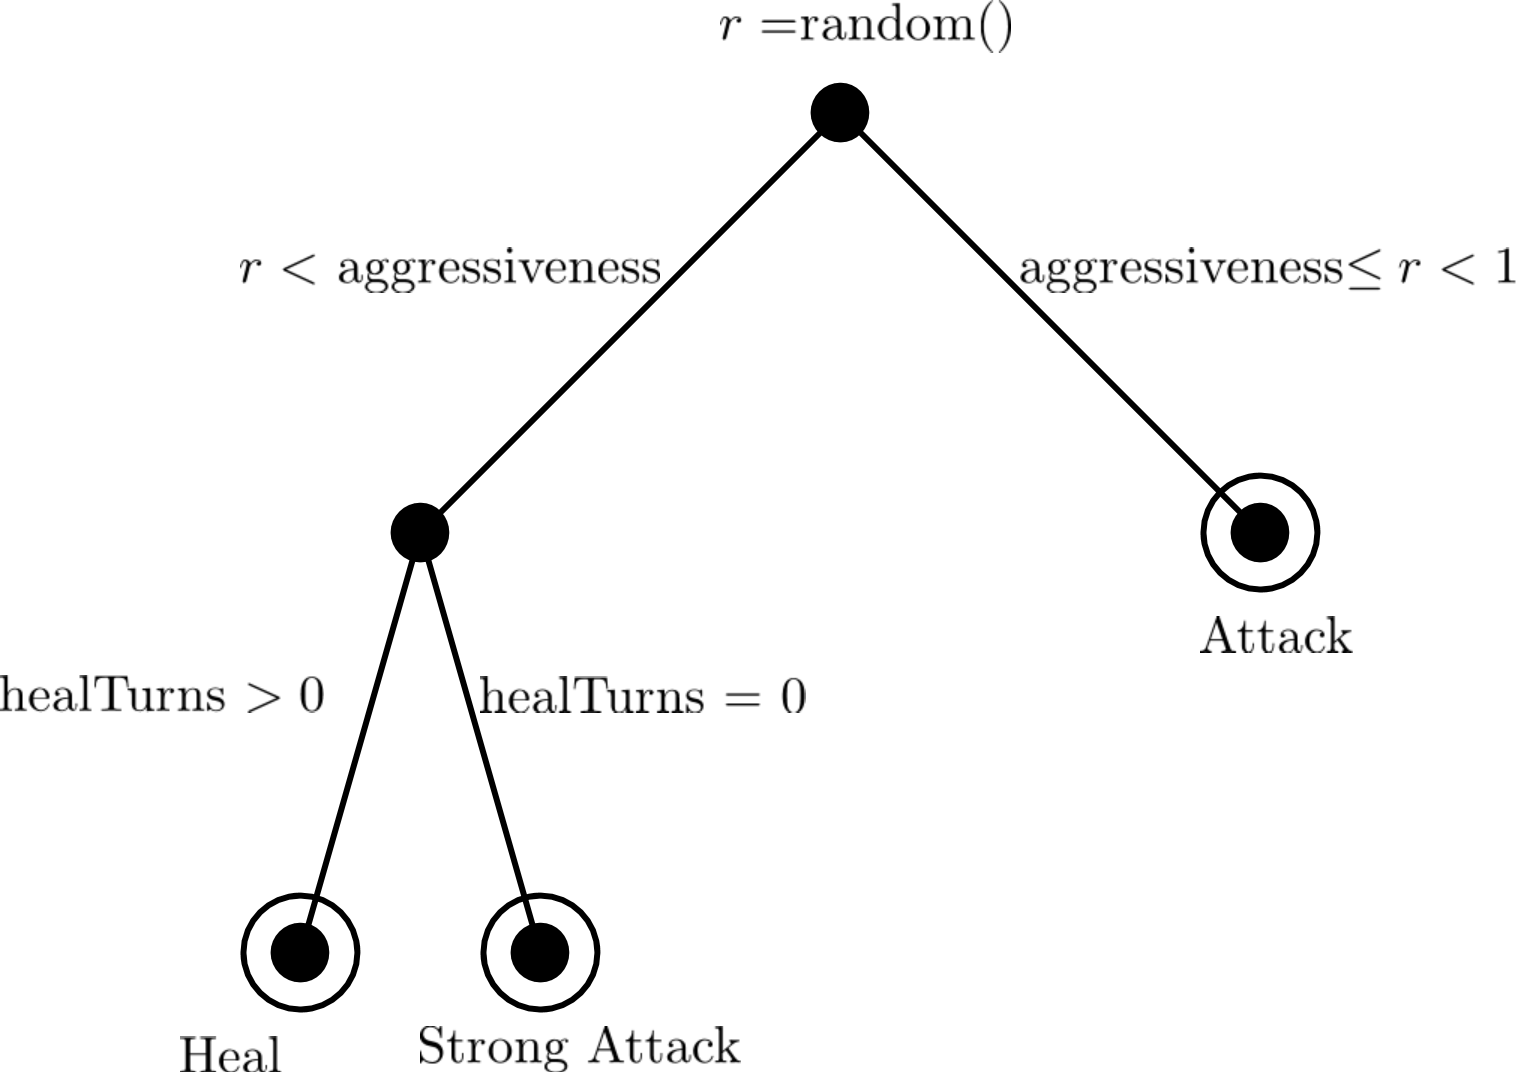
\includegraphics[width=8cm]{figures/AIAgressive.png}
  \caption{The decision tree for the \texttt{aggressiveRandomAI()} function.}
  \label{fig:AI3}
\end{figure}

The third model, \texttt{aggressiveRandomAI()}, is the final model which uses a random number generator. For this model, there is an additional variable given to the AI player, the aggressiveness stat. Rather than evenly splitting up actions 50-50, the choice between attacking and healing is split along this aggressiveness, which is a real number between 0 and 1. For this thesis, the aggressiveness was set to .25, leading to an AI which attacked 75\% of the time and healed 25\% of the time. As can be seen in the decision tree in Figure \ref{fig:AI3}, the AI uses strong attacks when the random number $r$ is below the aggressiveness stat and the two allotted healing turns are expended.

\lstset{language=python, label=lst:aggressiveAI, caption={The \texttt{aggressiveRandomAI()} function.}}
\begin{lstlisting}
# AI Model 3 - Use agressiveness statistic to determine how frequently the AI attacks.
# If the AI is randomly chosen to heal, but has expended all healing turns, it uses a
# strong attack instead.
def aggressiveRandomAI(self):
  newAction = ""
  r=random()
  if r<self.aggressiveness and self.healTurns > 0:
    newAction = "H"
  elif r<self.aggressiveness:
    newAction = "S"
  else:
    newAction = "A"
  return newAction
\end{lstlisting}

Like in the \texttt{randomAI()} function, the \texttt{aggressiveRandomAI()} function in Listing \ref{lst:aggressiveAI} is able to condense branches and nodes with \texttt{elif} and \texttt{else} statements. The \texttt{aggressiveness} variable is an element of the \texttt{PlayerAvatar} class, and is set to .25.

\begin{figure}[H]
  \centering
  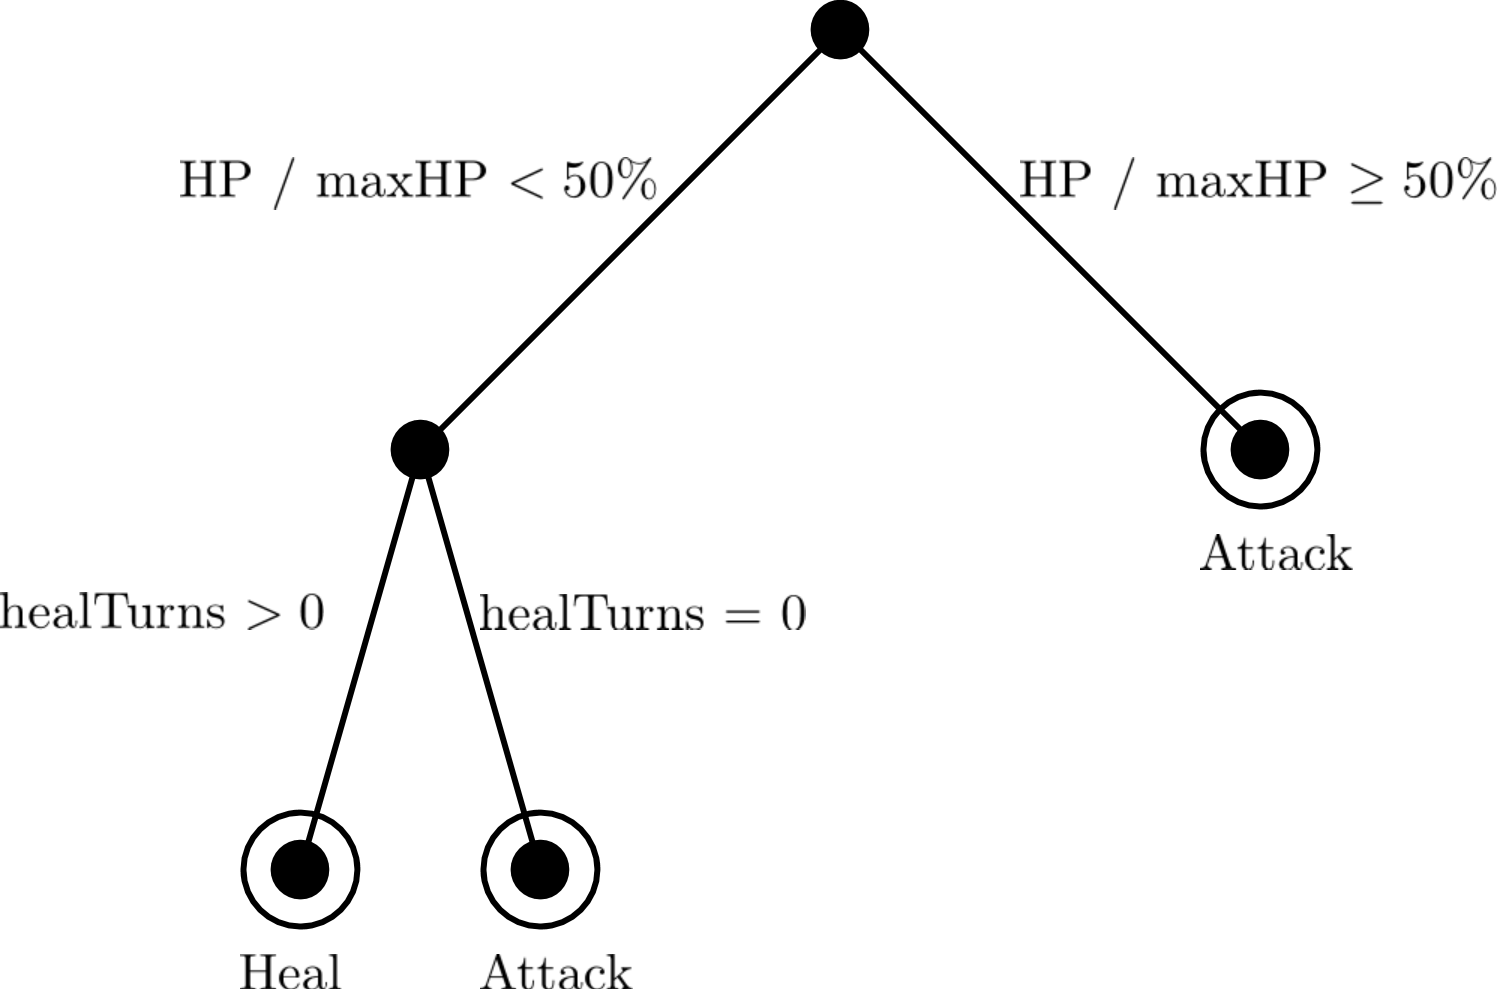
\includegraphics[width=8cm]{figures/AI50Percent.png}
  \caption{The decision tree for the \texttt{fiftyPercentAI()} function.}
  \label{fig:AI4}
\end{figure}

In the fourth model, \texttt{fiftyPercentAI()}, the AI only heals when its health falls below 50\% of its maximum. Thus, the AI only heals when it is close to death, as opposed to the random AI models which could potentially waste their heals at the start of a game. As shown in Figure \ref{fig:AI4}, this AI only uses normal attacks and heals; it does not do any parrying or strong attacks. Thus, it has the most in common with the \texttt{limitedRandomAI()} function with regards to possible actions. However, by saving heals until later in the game, this model has some semblance of intelligence, whereas the \texttt{limitedRandomAI()} does not.

\begin{figure}[H]
  \centering
  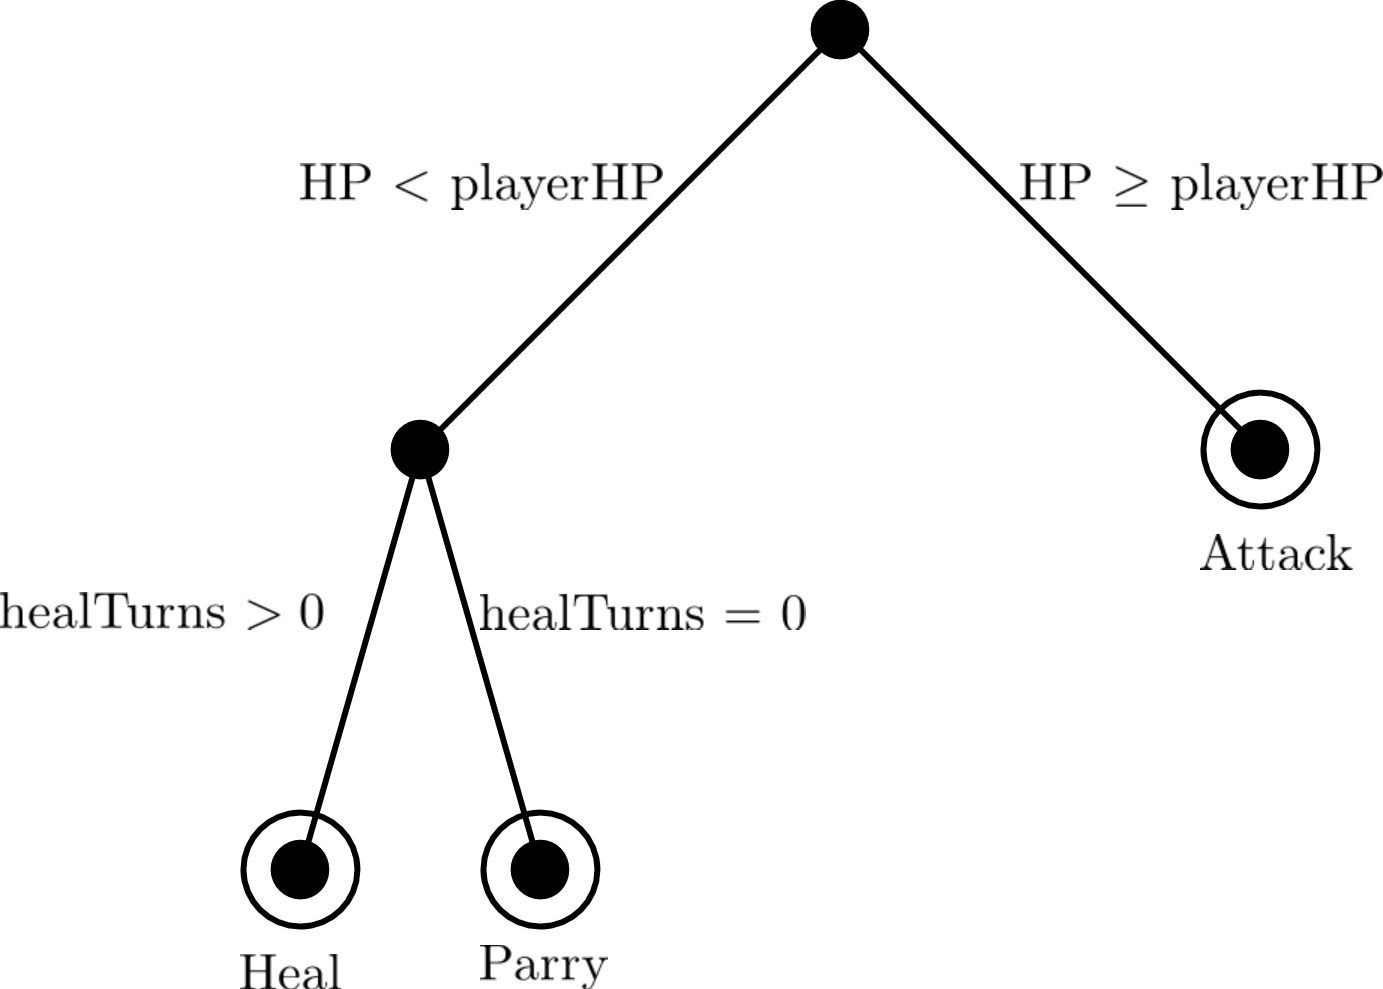
\includegraphics[width=8cm]{figures/AIComparative.png}
  \caption{The decision tree for the \texttt{comparativeAI()} function.}
  \label{fig:AI5}
\end{figure}

The fifth model uses similar tactics as the fourth, but instead of using 50\% as the threshold, the \texttt{comparativeAI()} function heals whenever its HP drops below the player's HP, as seen in Figure \ref{fig:AI5}. Additionally, when the AI has expended all its healing turns and its HP falls below the player's HP, the AI uses a parry instead of an attack. Over the course of a game, the AI will defend itself, relying on counter-attacks to weaken the player before making attacks of its own.

\begin{figure}[H]
  \centering
  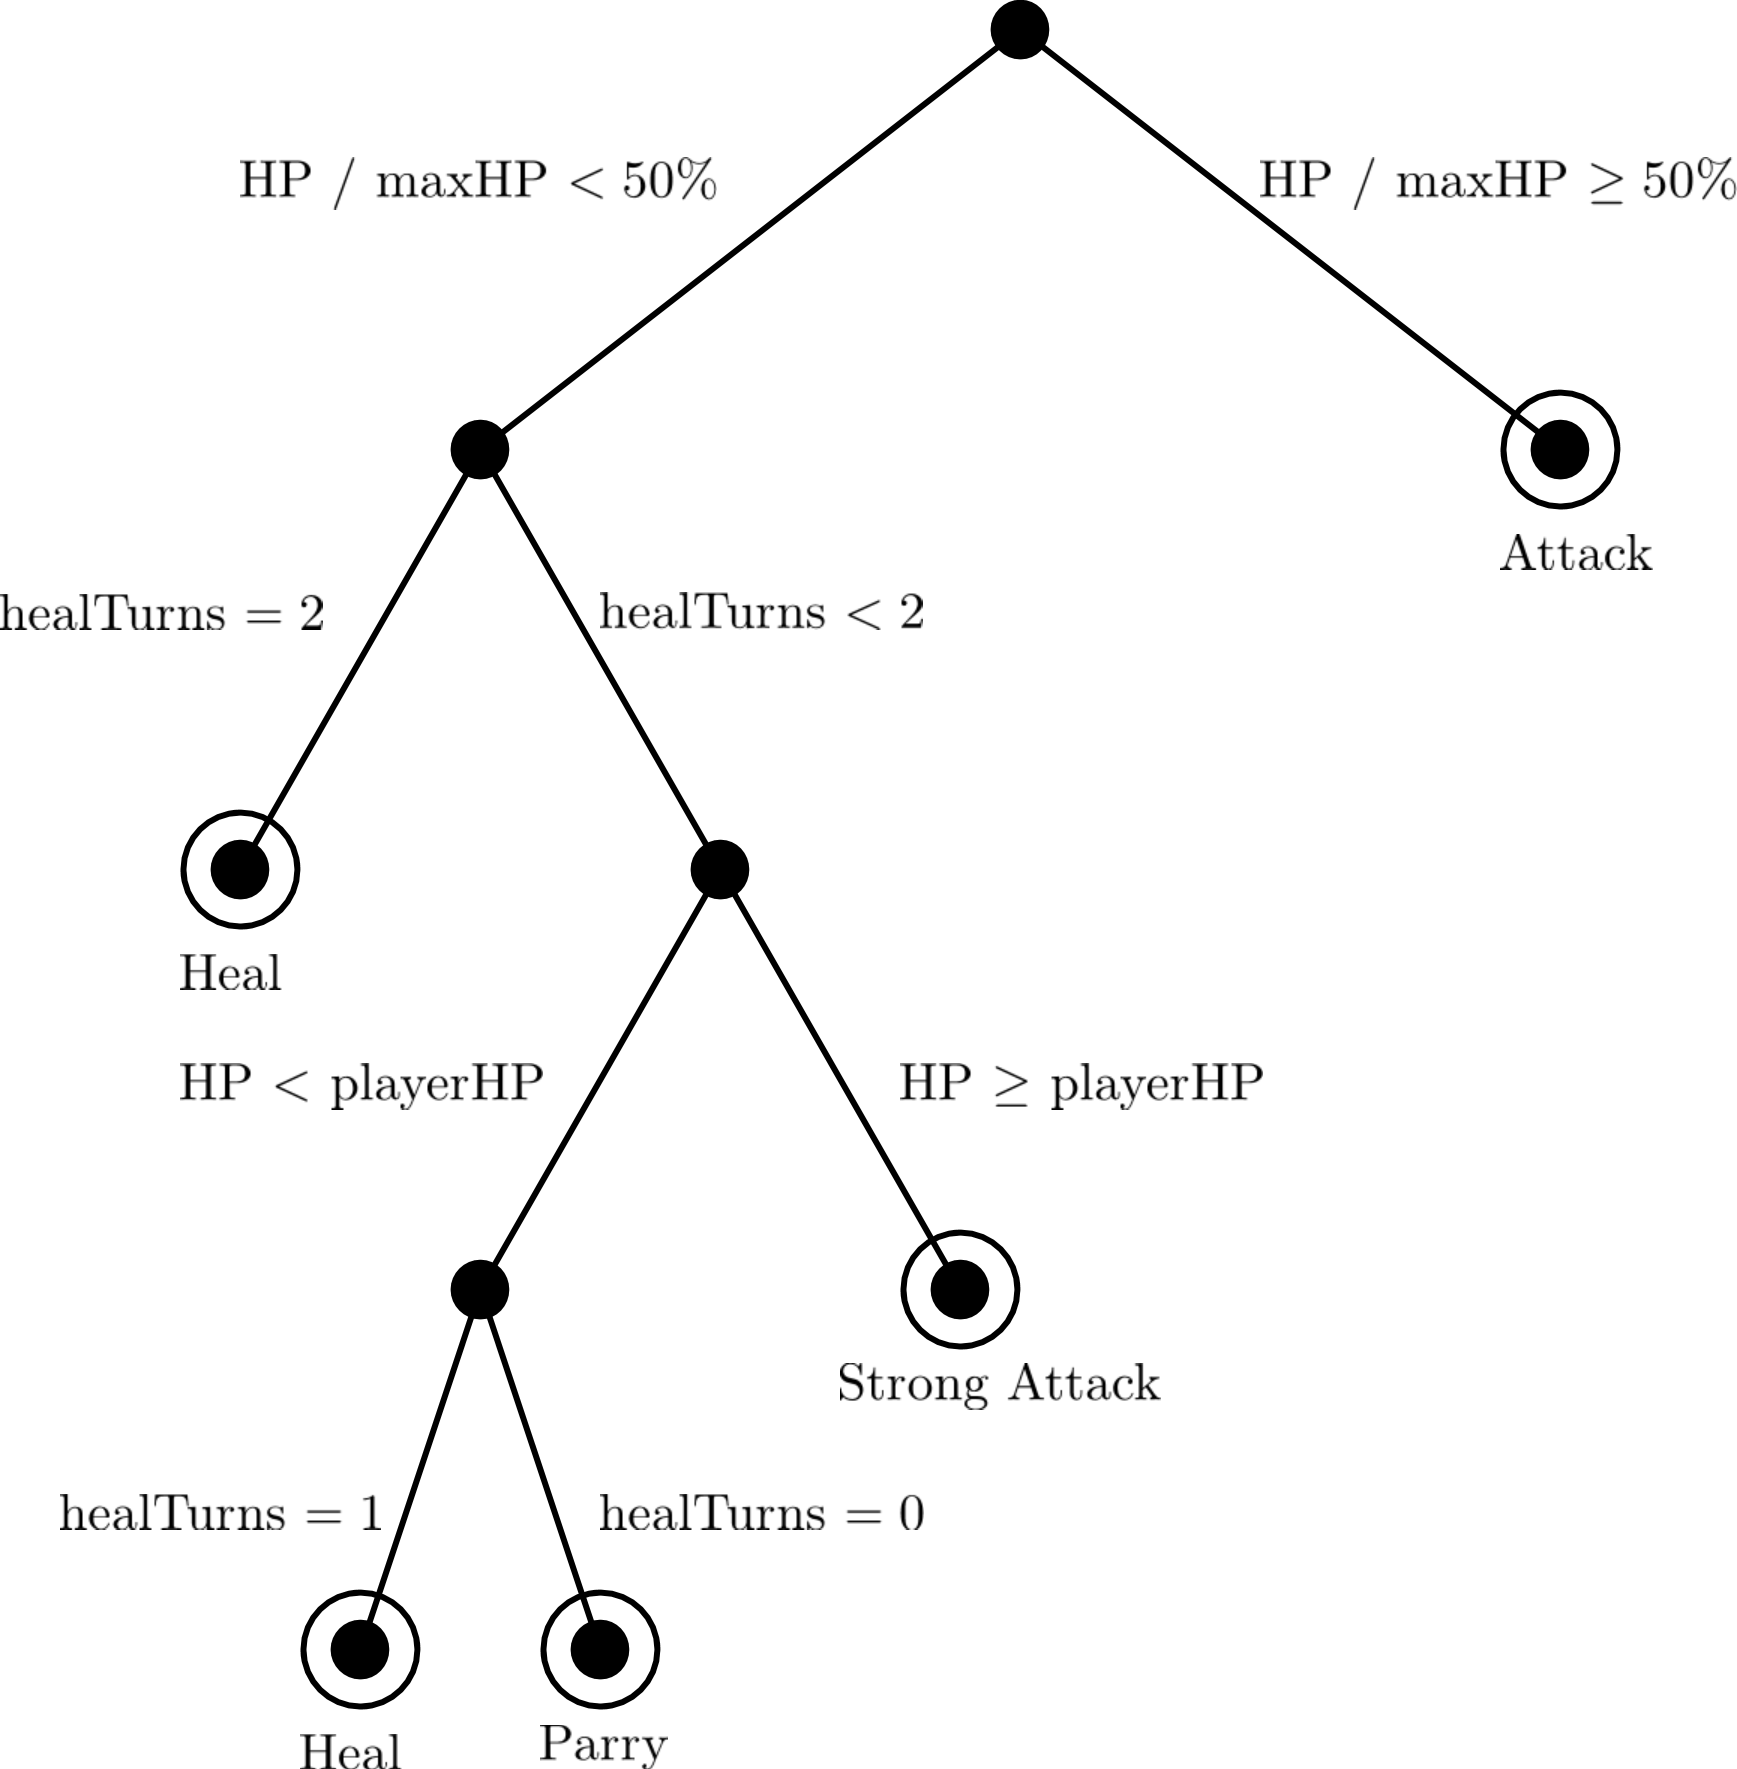
\includegraphics[width=9cm]{figures/AIScaling.png}
  \caption{The decision tree for the \texttt{scalingDifficulty()} function.}
  \label{fig:AI6}
\end{figure}

The \texttt{scalingDifficulty()} model in Figure \ref{fig:AI6} is a loose combination of the \texttt{fiftyPercentAI()} and \texttt{comparativeAI()} functions. As in \ref{fig:AI4}, the AI performs a normal attack whenever the AI's HP is above 50\% of its maximum. In this model, the two available healing turns are used in different circumstances. The first healing turn is used when the AI drops below 50\% HP for the first time. If their HP drops below 50\% after this first healing turn, the AI becomes more strategic. If the AI is below 50\% but still has a greater HP value than the player, then the AI will use strong attacks. However, if the AI is both below 50\% and below the player's HP, then it will use its second healing turn if available and parry if no healing turns remain.\\

\begin{figure}[H]
  \centering
  
\includegraphics[width=1cm]{figures/AIAttack.png}
  \caption{The decision tree for a baseline AI model, which only uses normal attacks.}
  \label{fig:AI7}
  \end{figure}

After some preliminary testing, the final two models were created. The first of these is a baseline model, which only uses normal attacks. As Figure \ref{fig:AI7} depicts, the decision tree for this model is a single leaf node.

\begin{figure}[H]
  \centering
  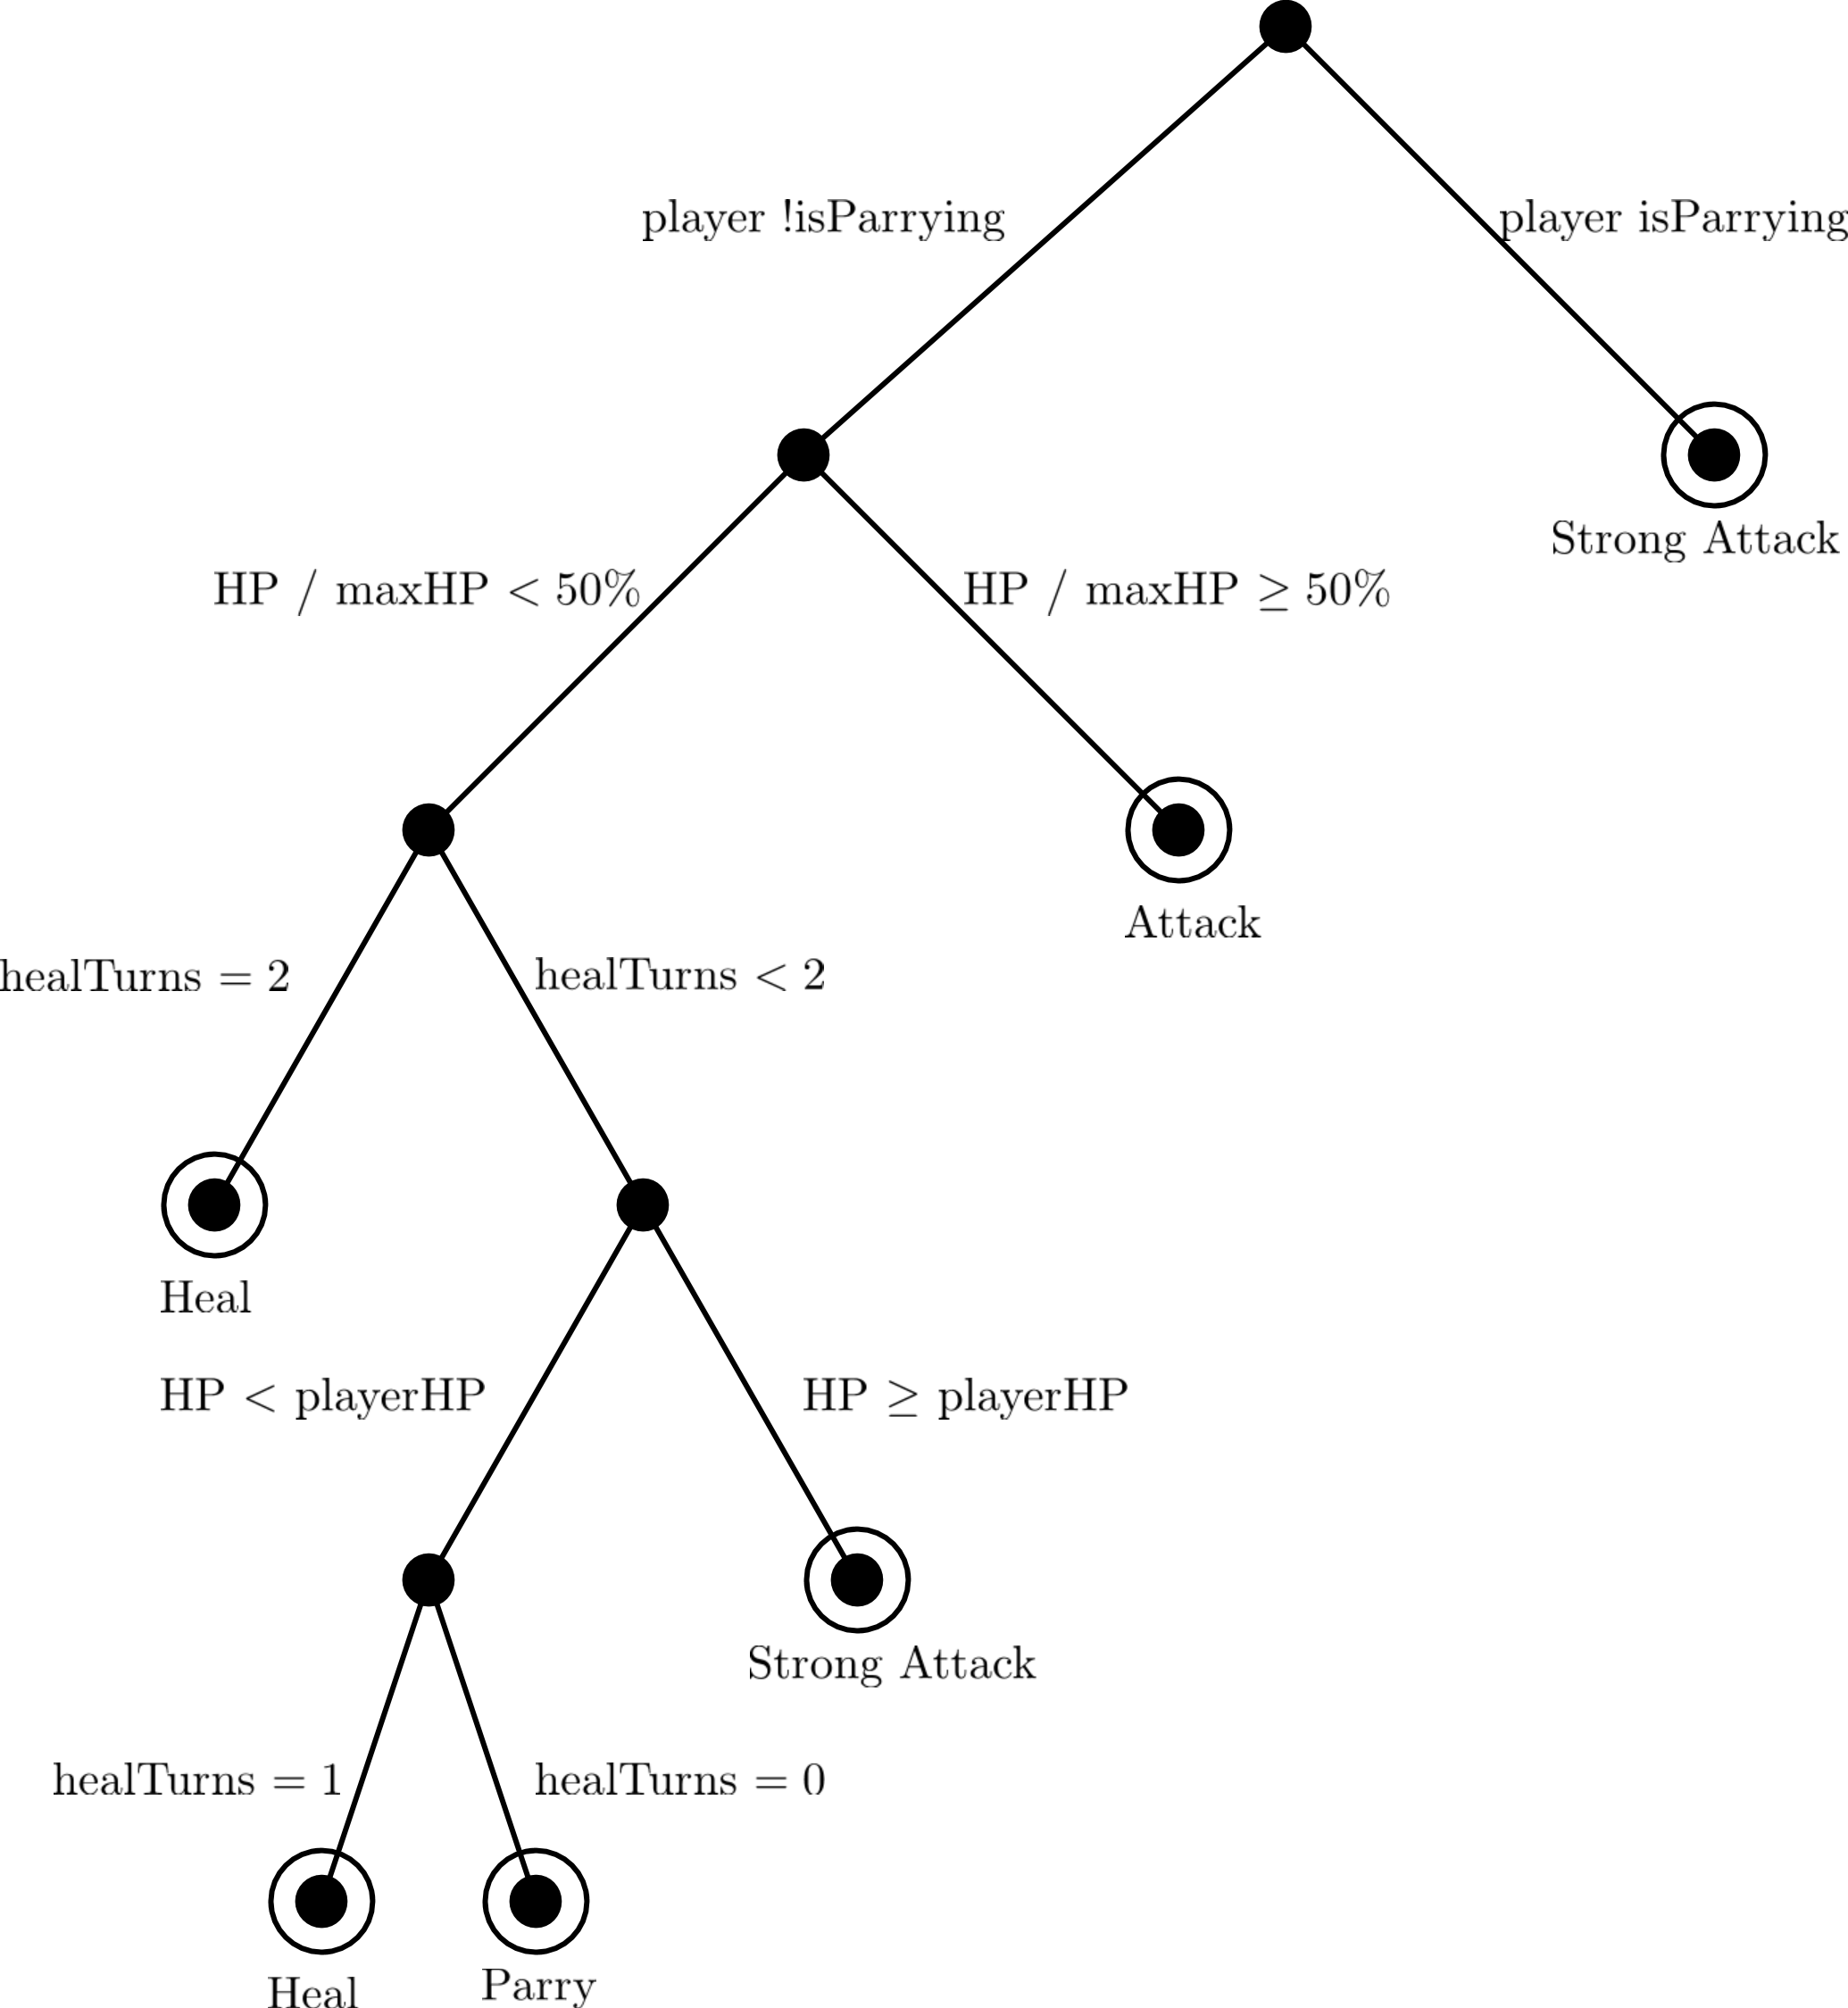
\includegraphics[width=10cm]{figures/AIParry.png}
  \caption{The decision tree for the \texttt{parryCountering()} function.}
  \label{fig:AI8}
\end{figure}
The second of these new models was designed to be more offensive and use strong attacks whenever the human player chose to parry. Otherwise, the second new model acts the same as the \texttt{scalingDifficulty} model.\\

\subsection{Visual Design}
The visual design of the game was left fairly simple, to avoid distracting players from the strategic elements of the game. Icons for the player character and enemy opponents were created in the GNU Image Manipulation Program (GIMP), then imported as pygame sprites using the \texttt{pygame.image.load()} function. Since these sprites had a transparency component, the function \texttt{convert\_alpha()} was also used to preserve this transparency in pygame.\\

\begin{figure}[H]
  \centering
  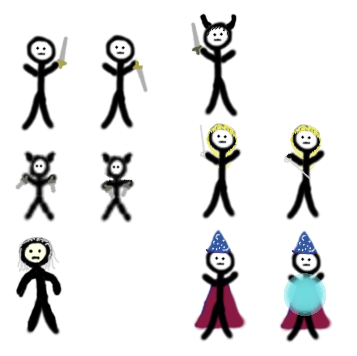
\includegraphics[width=10cm]{sprites/SpriteSheet.png}
  \caption{The set of sprites used for the characters in \textit{Cave Escape}. Clockwise from top left: the player character, an orc, an elf, a beserker, a knight, a magician, a troll, and a goblin.}
  \label{fig:SpriteSheet}
\end{figure}

\begin{figure}[H]
  \centering
  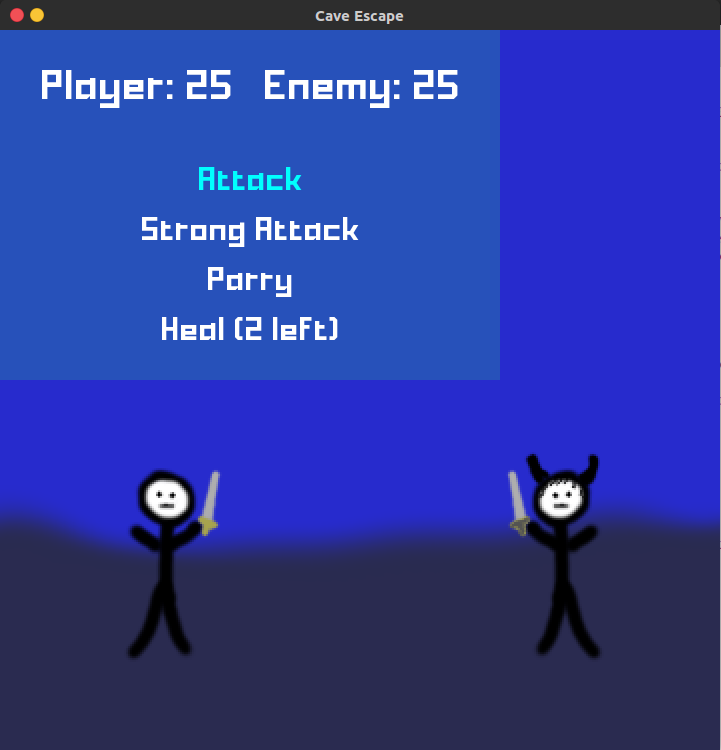
\includegraphics[width=6.5cm]{figures/In-Game.png}
  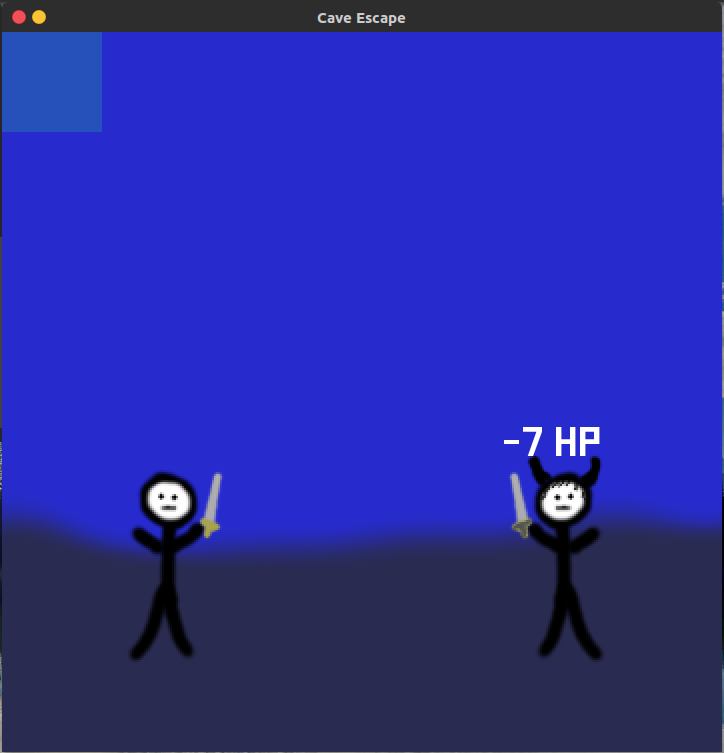
\includegraphics[width=6.5cm]{figures/In-Game2.png}
  \caption{In-game screenshots from \textit{Cave Escape}. The player character is situated on the left, while the opponent - an orc - is stationed on the right. The HP values of both player and AI are listed at the top of the screen. In the left image, the player is able to select their next move from the list of options. In the right image, the player has selected ``Strong Attack'' and the resulting damage is shown above the enemy's head.}
  \label{fig:ingame}
\end{figure}

An individual sprite was created for the player character and each of the five AI models, as shown in Figure \ref{fig:SpriteSheet}. These sprites are overlaid on a bluish-purple background symbolizing the cave interior. The list of possible actions is also shown on-screen, positioned above the player character as in Figure \ref{fig:ingame}. Next to the ``Heal'' option, the number of remaining healing turns is listed and updated after each turn. The HP of both players is also updated after every turn. Additionally, after players select an action, the resulting change in HP is shown above the head of the respective target. The right image in Figure \ref{fig:ingame} shows that the orc was hit by a strong attack made by the player, and took 7 points of damage.\\

Each non-player character has a respective AI model which it uses. The goblin uses the \texttt{randomAI()} function in Figure \ref{fig:AI2}. The troll uses \texttt{aggressiveRandomAI()}, as seen in Figure \ref{fig:AI3}. The orc uses the \texttt{fiftyPercentAI()} function from Figure \ref{fig:AI4}. The elf is assigned to the \texttt{comparativeAI()} function seen in Figure \ref{fig:AI5}, and the magician uses the \texttt{scalingDifficulty()} function from Figure \ref{fig:AI6}. The baseline model in Figure \ref{fig:AI7} is assigned to the beserker, and the \texttt{parryCountering()} function in Figure \ref{fig:AI8} is assigned to the knight.

\begin{figure}[H]
  \centering
  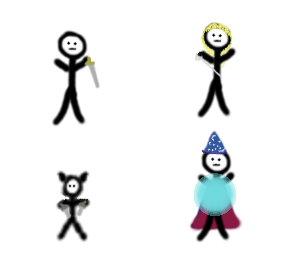
\includegraphics[width=8cm]{sprites/ParrySheet.png}
  \caption{The set of sprites used when a character is parrying. Five of the characters are able to parry. Clockwise from top left: the player character, a goblin, an elf, a knight and a magician.}
  \label{fig:ParrySheet}
\end{figure}

In addition to the default sprites shown in Figure \ref{fig:SpriteSheet}, characters have a second sprite for when they are parrying. The Troll, Orc, and Beserker characters are unable to parry, so only five of these sprites were created. These variants are shown in Figure \ref{fig:ParrySheet}: the player character, the goblin, the elf, the knight, and the magician all have parry sprites.\\

At runtime, the game starts at a menu screen, where the five enemy characters are listed. When the HP of either the player or the AI falls to 0 or lower, the round ends. A final screen is shown to either celebrate the player's victory or lament their failure. The menu was made using code from a \textit{Tetris} clone made with pygame created by Dimitris Strovolidis, released under the GNU General Public License, version 3 \cite{tetris}. This code contains a \texttt{menu} class which allows both for interactive menus and easily-positioned text. The enemy characters are listed in this menu, and players are able to select which opponent they wish to fight. Both this title menu and the in-game action menus shown in Figure \ref{fig:ingame} use this \texttt{menu} class.

\section{Playtesting and Survey}
To test the effectiveness of these AI models, a group of participants were surveyed to play the various models. Each participant played five rounds against one of the models. The program collects data on wins and losses, as well as the sequence of actions taken by both the human player and the AI opponent. In addition to this game data, a short survey was given to each participant. Subjects were asked to answer the first three questions before playing the game. These questions asked participants to rate, on a scale of 1 to 5, their interests in video games, strategic board games, and RPGs, respectively. A score of 1 indicated little or no interest, while a score of 5 indicated a strong interest. After the three questions, participants were given a short description of the game, including the possible actions that players could take in the game. After the participant completed the five rounds, they were asked three more questions. These questions asked them to rate, on a scale of 1 to 5, how fun they found the game, how understandable the controls were, and how aggressively or passively they played. 1 indicates a rating of not fun, that the controls were not understandable at all, and that the player used a very passive playstyle, respectively. A 5 rating indicated that the participant greatly enjoyed the game, that the controls were very understandable, and that their playstyle was very aggressive, respectively.\\

% Table generated by Excel2LaTeX from sheet 'Sheet1'
\begin{table}[hbtp]
  \centering
  \begin{tabular}{|rlrrr|rrr|}
    \toprule
    \rowcolor[rgb]{ 0,  0,  0} \multicolumn{1}{|l}{\textcolor[rgb]{ 1,  1,  1}{\textbf{Test \#}}} & \textcolor[rgb]{ 1,  1,  1}{\textbf{AI Model}} & \multicolumn{1}{l}{\textcolor[rgb]{ 1,  1,  1}{\textbf{Q1}}} & \multicolumn{1}{l}{\textcolor[rgb]{ 1,  1,  1}{\textbf{Q2}}} & \multicolumn{1}{l}{\textcolor[rgb]{ 1,  1,  1}{\textbf{Q3}}} & \multicolumn{1}{l}{\textcolor[rgb]{ 1,  1,  1}{\textbf{Q4}}} & \multicolumn{1}{l}{\textcolor[rgb]{ 1,  1,  1}{\textbf{Q5}}} & \multicolumn{1}{l|}{\textcolor[rgb]{ 1,  1,  1}{\textbf{Q6}}} \\
    \midrule
    \rowcolor[rgb]{ .851,  .851,  .851} \textbf{1} & Goblin & 3.5   & 5    & 4     & 3     & 5     & 5 \\
    \midrule
    \textbf{2} & Troll & 5     & 5     & 5       & 4     & 5     & 3 \\
    \midrule
    \rowcolor[rgb]{ .851,  .851,  .851} \textbf{3} & Orc   & 4     & 4     & 5       & 5     & 5     & 3 \\
    \midrule
    \textbf{4} & Elf   & 4     & 5     & 4      & 4     & 5     & 1 \\
    \midrule
    \rowcolor[rgb]{ .851,  .851,  .851} \textbf{5} & Magician  & 5     & 3     & 4     & 5     & 5     & 4 \\
    \midrule
    \textbf{6} & Goblin & 5     & 5     & 5   & 3     & 5     & 4 \\
    \midrule
    \rowcolor[rgb]{ .851,  .851,  .851} \textbf{7} & Troll & 4     & 4     & 5     &   3     & 5     & 5 \\
    \midrule
    \textbf{8} & Orc   & 5     & 5     & 5    & 4     & 5     & 4 \\
    \midrule
    \rowcolor[rgb]{ .851,  .851,  .851} \textbf{9} & Elf   & 2     & 3     & 1      & 4     & 5     & 4 \\
    \midrule
    \textbf{10} & Magician & 2     & 2     & 1     & 2     & 4     & 3 \\
    \midrule
    \rowcolor[rgb]{ .851,  .851,  .851} \textbf{11} & Goblin & 4     & 5     & 4     & 5     & 3     & 5 \\
    \midrule
    \textbf{12} & Troll & 1     & 2     & 1     & 2     & 3     & 3 \\
    \midrule
    \rowcolor[rgb]{ .851,  .851,  .851} \textbf{13} & Orc   & 3     & 3     & 5    & 5     & 5     & 3 \\
    \midrule
    \textbf{14} & Elf   & 3     & 4     & 2         & 3     & 5     & 5 \\
    \midrule
    \rowcolor[rgb]{ .851,  .851,  .851} \textbf{15} & Magician  & 4     & 3     & 3    & 4     & 5     & 4 \\
    \midrule
    \textbf{16} & Goblin & 2     & 2     & 2      & 5     & 5     & 4 \\
    \midrule
    \rowcolor[rgb]{ .851,  .851,  .851} \textbf{17} & Beserker & 5     & 3     & 5      & 4     & 5     & 3 \\
    \midrule
    \textbf{18} & Knight & 5     & 4     & 4      & 5     & 5     & 4 \\
    \midrule
    \rowcolor[rgb]{ .851,  .851,  .851} \textbf{19} & Beserker & 5     & 4     & 5     & 3     & 4     & 2 \\
    \midrule
    \textbf{20} & Knight & 4     & 3     & 3      & 4     & 5     & 4 \\
    \midrule
    \rowcolor[rgb]{ .851,  .851,  .851} \textbf{21} & Knight & 5     & 3     & 5      & 5     & 5     & 4 \\
    \bottomrule
  \end{tabular}%
  \caption{Results of the survey given to all playtesters of \textit{Cave Escape}. For each question, participants rated themselves on a scale of 1 to 5. The first three questions were asked before participants played the game. Q1 asks participants their interest in video games; Q2 asks their interest in strategic board games; Q3 asks their interest in RPGs. After participants played 5 rounds of the game, they answered the last three questions. Q4 asks participants their enjoyment of the game; Q5 asks their understanding of the controls; Q6 asks participants to rate the aggressiveness or defensiveness of their playstyle.}
  \label{tab:survey}%
\end{table}%

Most of the AI models were played by three participants, except the Goblin - which was tested by four participants - and the Beserker - which was tested by two participants. The responses given by the survey participants are recorded in Table \ref{tab:survey}. On average, survey participants rated themselves as having 3.5 out of 5 for interest in video games, 3.75 out of 5 for interest in strategic board games, and 3.5 out of 5 for interest in RPGs. In the post-game survey, participants rated the game 3.8 out of 5 for fun, and rated the controls a 4.6 out of 5 for ease of comprehension. For their own playstyle, players on average rated themselves 3.75 out of 5, indicating that the average playstyle was a fairly even mix of offensive and defensive choices, with a slight edge toward offensive.\\

\begin{figure}[H]
  \centering
  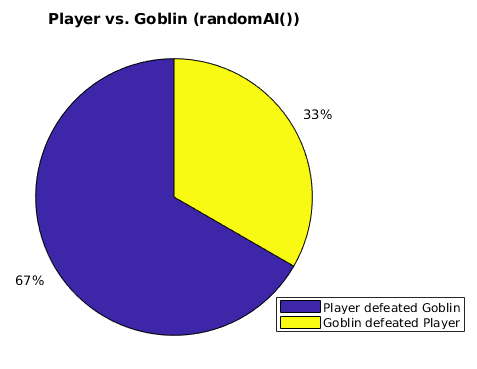
\includegraphics[width=7.75cm]{figures/goblinWins.png}
  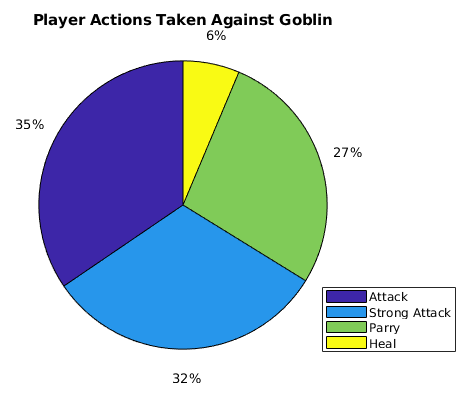
\includegraphics[width=7cm]{figures/actionsGoblin.png}
  \caption{On left, the win/loss percentages for the randomAI() function, assigned to the Goblin character. On right, the percentage of actions players used against the Goblin.}
  \label{fig:pieGoblin}
\end{figure}
After 20 individual games against the Goblin AI - using the randomAI function - the win percentage for the survey participants are as shown in the left chart in Figure \ref{fig:pieGoblin}: a 67\% win percentage for the human player, and a 33\% win percentage for the Goblin. Since this AI model uses a random number generator to determine its actions, this win percentage suggests that unpredictability is more difficult for human players to defeat. Furthermore, we can see that the expanded version of the game, with 25 HP instead of 10 and two more abilities, has more outcomes where player 2 can win.\\

Participants who played this AI model rated their enjoyment on average as 4 out of 5. These same participants rated their playstyle as 4.5 out of 5, indicating that they played very aggressively. However, as shown in the right chart of Figure \ref{fig:pieGoblin}, players actually had a fairly even split between normal attacks, strong attacks, and parries. Healing, since it is limited to twice per round, is necessarily less common. While as a whole players did opt to use offensive moves instead of defensive moves, their aggression is somewhat overstated.

\begin{figure}[H]
  \centering
  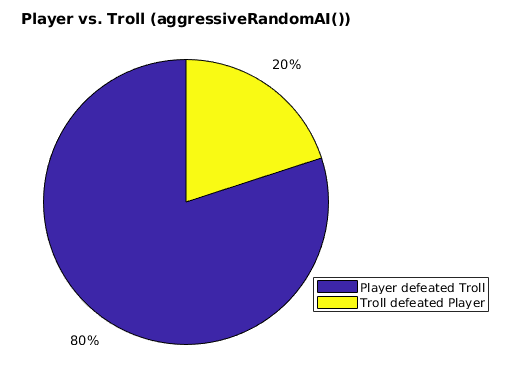
\includegraphics[width=8cm]{figures/trollWins.png}
  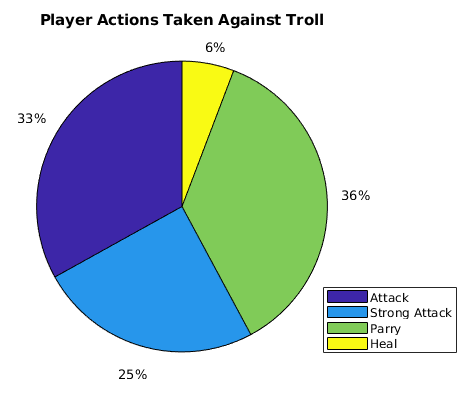
\includegraphics[width=7cm]{figures/actionsTroll.png}
  \caption{On left, the win/loss percentages for the aggressiveRandomAI() function, assigned to the Troll character. On right, the percentage of actions players used against the Troll.}
  \label{fig:pieTroll}
\end{figure}

The Troll AI fared much worse than the Goblin, as seen in the left chart of Figure \ref{fig:pieTroll}. The aggressive AI was only able to win 20\% of its games. In comparison to the Goblin, the Troll is less likely to use strong attacks; the Goblin can use a strong attack whenever, but the Troll must first expend both of their healing turns before it can use a strong attack. Additionally, the Goblin can parry while the Troll cannot. Thus, at any particular turn of the game, the Troll has a more limited move set than the Goblin.\\

Participants who played this AI model rated their enjoyment on average as 3 out of 5, the lowest of all the models. On average, they rated their playstyle as 2.75 out of 5, indicating that they leaned towards defensive playstyles. In comparison to the actions taken against the Goblin in the right chart of Figure \ref{fig:pieGoblin}, this self-identification is correct: players who fought the Troll tended to parry more than players who fought the Goblin, as shown on the right chart of Figure \ref{fig:pieTroll}. Players who fought the Goblin parried 27\% of the time, while players who fought the Troll parried 36\% of the time.\\

Since the Troll primarily uses normal attacks, this increase in parrying is to be expected. With such an increase, we can infer that players were able to guess at the decisions made by the Troll, and expected the Troll to use normal attacks. This is supported by the win/loss percentages as well, as players were more successful fighting the Troll than the Goblin.

\begin{figure}[H]
  \centering
  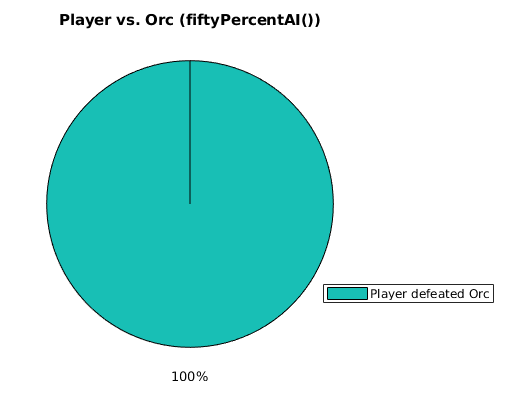
\includegraphics[width=7cm]{figures/orcWins.png}
  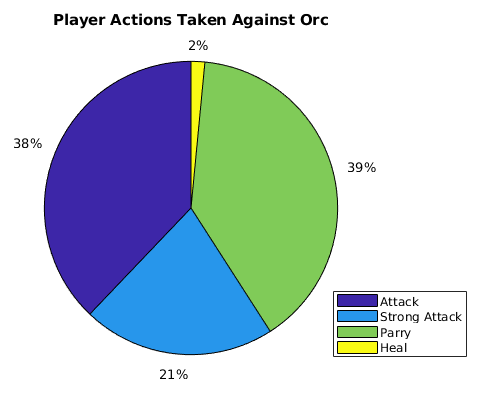
\includegraphics[width=7cm]{figures/actionsOrc.png}
  \caption{On left, the win/loss percentages for the fiftyPercentAI() function, assigned to the Orc character. On right, the percentage of actions players used against the Orc.}
  \label{fig:pieOrc}
\end{figure}

The Orc AI performed the worst of all, as is evident from the left chart of Figure \ref{fig:pieOrc}. Not a single person lost to the Orc after 15 trials. The Orc also has the most limited move set of these first three models, only able to heal and use normal attacks. Seeing as the Orc has the same available moves as the players in the simple simulation in Figure \ref{fig:gameTree}, it is unsurprising that the Orc has trouble winning games.\\

Participants who played this AI model rated their enjoyment on average as 4.6 out of 5. They rated their playstyle as 3.3 out of 5, indicating that they leaned towards aggressive play, but were slightly more defensive than players who fought the Troll. As shown in the right chart of Figure \ref{fig:pieOrc}, players who fought the Orc healed less often than players who fought the Goblin or Troll, but parried more than those same players. This data suggests that players did not feel as threatened by the Orc as they did the Troll or Goblin. As with the Troll, the Orc relies on normal attacks. Furthermore, unlike the Troll, the Orc does use any strong attacks which would counteract a player's parry. Thus, players can once again guess at the decisions made by the Orc. Given that the Orc did not win a single battle, these players appear to be correct.\\

\begin{figure}[H]
  \centering
  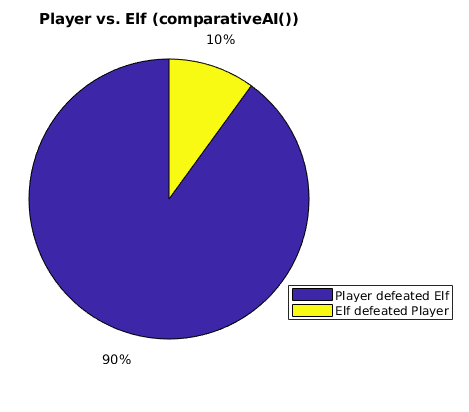
\includegraphics[width=7.25cm]{figures/elfWins.png}
  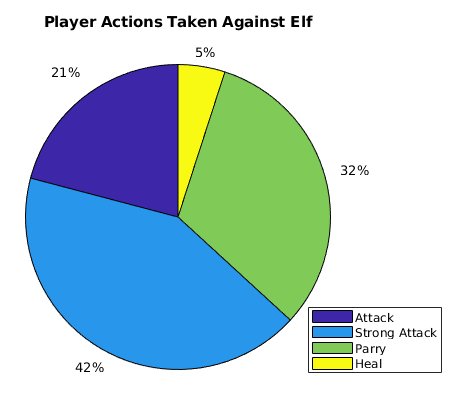
\includegraphics[width=7cm]{figures/actionsElf.png}
  \caption{On left, the win/loss percentages for the comparativeAI() function, assigned to the Elf character. On right, the percentage of actions players used against the Elf.}
  \label{fig:pieElf}
\end{figure}

The left chart of Figure \ref{fig:pieElf} shows that the comparativeAI() function was only slightly successful. Human players won 93\% of the games while the AI won 7\% of the games. Since this model uses parries frequently, a player is able to safely heal themselves without immediately losing that HP on the Elf's next attack. Furthermore, a successful parry deals 3 points of damage while a successful strong attack deals 7 points of damage. If a player chooses to use a normal attack twice followed by a strong attack, they will lose 6 HP from the Elf's parries but will still have a net gain of 1 HP. Thus, a player can take a few hits from parries but still come out ahead with strong attacks. This difference gives players the opportunity to learn that strong attacks cannot be parried.

As seen in the right chart of Figure \ref{fig:pieElf}, players who fought the Elf used more strong attacks than against any of the AI opponents. Since the Elf tries to parry after it runs out of healing turns, the number of strong attacks predictably increases as players try to break through their opponent's parry. While not as low as against the Orc, players who fought the Elf chose to heal slightly less than against the Goblin and Troll. Since the Elf is on the defense for much of each round, players are likely basing their decisions on ways to break through the Elf's parry and not on keeping their character alive. On average, players who fought this AI model rated their enjoyment of the game 3.5 out of 5. This rating is lower than the ratings for both the Goblin and Orc models, but higher than the rating for the Troll model. While the decisions made by the Elf are more complicated than the Goblin, the Elf's reliance on parrying impacted the enjoyment of the participants; participants seem to have more enjoyment playing AI models which were more active. Players rated their own strategy as a 3 out of 5 in terms of offensive and defensive. In comparison to the data, players actually used attacks (both normal and strong) 63\% of the time, and used defensive moves (healing and parrying) 37\% of the time. It is possible that, given that the Elf chooses to parry on most of its actions, players view this battle as more guarded than others. The Elf's defensive stance may give players the impression of a duel between two skilled opponents, with each looking to exploit an opening; this is in contrast with the Orc and Troll battles, where players alternate with attacks until one falls. Thus, even though the data tells a different story, players felt that they were more cautious when battling the Elf than against the Orc and Troll.

\begin{figure}[H]
  \centering
  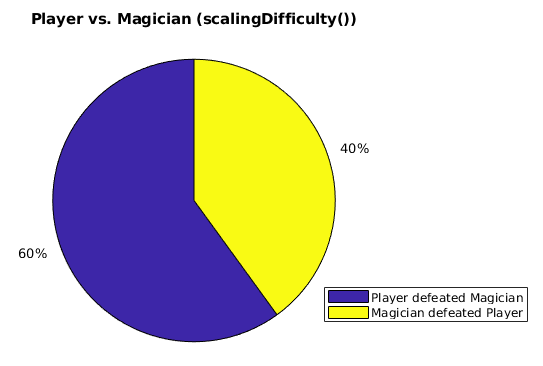
\includegraphics[width=8.5cm]{figures/magicianWins.png}
  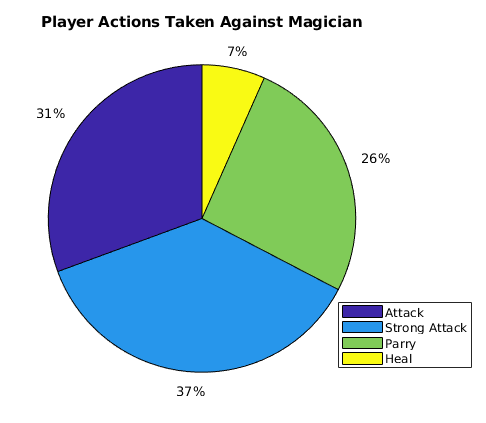
\includegraphics[width=6.5cm]{figures/actionsMagician.png}
  \caption{On left, the win/loss percentages for the scalingDifficulty() function, assigned to the Magician character. On right, the percentage of actions players used against the Magician.}
  \label{fig:pieMagician}
\end{figure}

The Magician character has one of the best overall records, as seen in the left chart of Figure \ref{fig:pieMagician}: a win rate of 60\% for the player and 40\% for the Magician. Like the Goblin, the Magician is able to perform all four of the available actions, which the other three AI models could not do. Given the similar win/loss rates for the Goblin and Magician, it may be the case that, by limiting the available actions for the other AI models, they were handicapped in a way that the Goblin and Magician were not.\\

Players who fought the magician rated their enjoyment on average as 3.6 out of 5, and rated their playstyle as 3.6 out of 5 as well. This playstyle value indicates players chose offensive moves slightly more often than defensive moves. As with the Elf, the Magician's choice to parry at low health levels forces players to use strong attacks to win the game. Since the Magician parries less often than the Elf, players used fewer Strong Attacks against the Magician than they did against the Elf. Furthermore, players parried less often against the Magician than against the Elf. This data supports the self-identification of the participants' playstyle. Since the threshold for when the Magician starts parrying is lower than the same threshold for the Elf, players can afford to be more aggressive while fighting the Magician. 

\begin{figure}[H]
  \centering
  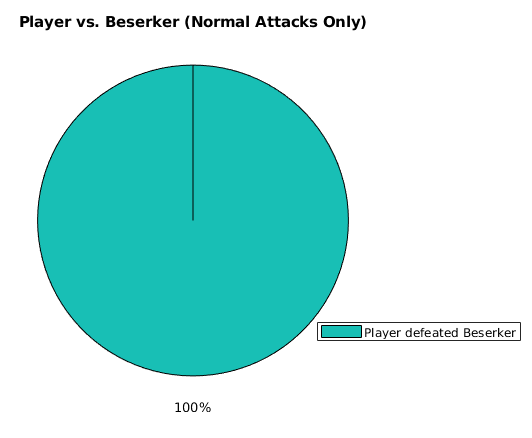
\includegraphics[width=7.5cm]{figures/beserkerWins.png}
  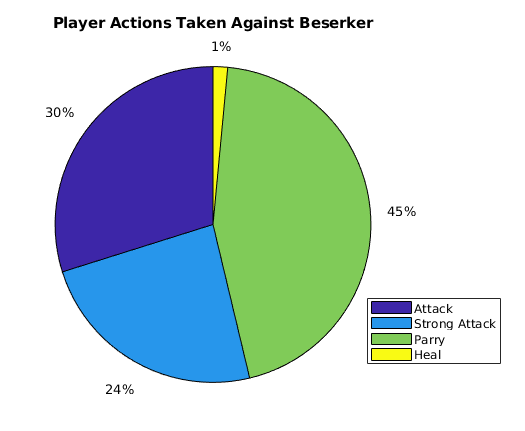
\includegraphics[width=7.5cm]{figures/actionsBeserker.png}
  \caption{On left, the win/loss percentages for the baseline AI model, which only uses normal attacks. This AI model is designated as the Beserker. On right, the percentage of actions players used against the Beserker.}
  \label{fig:pieBeserker}
\end{figure}

The Beserker, like the Orc, did not win a single battle. As a baseline model, the Beserker only used normal attacks. Compared to other AI models, it is most similar to the Orc, but without the healing turns taken when the model's HP drops below 50\%. As shown in the right chart of Figure \ref{fig:pieBeserker}, players who fought this AI model chose to heal less often and parried more often against the Beserker than against any other AI model.\\

Players who fought the Beserker rated their enjoyment on average as 3.5 out of 5. These participants rated their playstyle as 2.5 out of 5, indicating a mostly defensive playstyle. This was the most defensive rating that players gave for any of the AI models. Given that these players chose to parry on 45\% of their turns, the data supports the participants' ranking.

\begin{figure}[H]
  \centering
  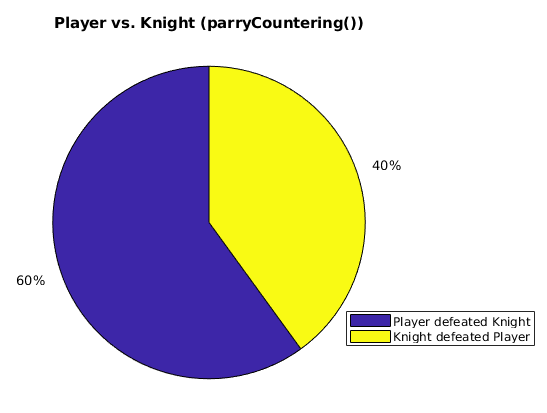
\includegraphics[width=7.5cm]{figures/knightWins.png}
  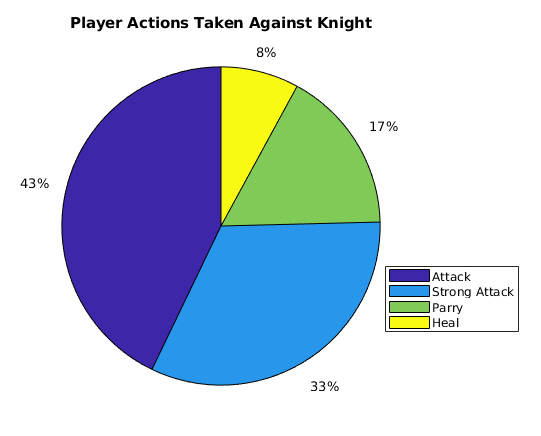
\includegraphics[width=7cm]{figures/actionsKnight.png}
  \caption{On left, the win/loss percentages for the \texttt{parryCountering()}  function, assigned to the Knight character. On right, the percentage of actions players used against the Knight.}
  \label{fig:pieKnight}
\end{figure}

The Knight AI model performed comparatively to the Magician AI. As shown on the left chart of Figure \ref{fig:pieKnight}, participants were able to defeat the Knight in 60\% of the tests while the Knight defeated players in 40\% of the tests.\\

Participants ranked their enjoyment on average as 4.6 out of 5; they ranked their playstyle as 4 out of 5, indicating mostly aggressive play. The only major difference between the Knight and the Magician models is the Knight's choice to use Strong Attacks any time that the player parries. As shown in the right chart of Figure \ref{fig:pieKnight}, participants learned quickly not to attempt to parry; at 17\%, players parried less often against the Knight than against any other AI model. Additionally, players healed more often while fighting the Knight than against any other AI model. In terms of offense, players used normal attacks more often than against any other AI model as well. In total, the data shows that players relied on the certainty of a normal attack, rather than deal with the possibility of a miss with a strong attack. This data, as well as the high ranking participants gave their aggression, suggests that players felt threatened by the Knight model.

While the player can choose their actions to play strategically, some of the AI models can be easily beaten if the player chooses to use normal attack every turn. In casual observation, the Troll, Orc, and Beserker can be reliably beaten by only attacking. The Goblin can occasionally be defeated with only normal attacks, but will occasionally defeat the player. Like the early version of the game explored in Figure \ref{fig:gameTree}, the human player has a tremendous advantage by taking the first turn. However, the addition of parries and strong attacks allows for second player in this version of the game to win, while the second player in the first version could only win if Player 1 chose to heal at specific moments. If the human player chooses to only attack, the Magician, Elf, and Knight cannot be defeated. Since they stop parrying if their HP is above the player's HP, these AI models are able to stay ahead.

\begin{table}[htbp]
  \centering
  \begin{tabular}{|c r|}
    \toprule
    \rowcolor[rgb]{ 0,  0,  0} \multicolumn{1}{|l}{\textcolor[rgb]{ 1,  1,  1}{\textbf{AI Model}}} & \textcolor[rgb]{ 1,  1,  1}{\textbf{Average Player HP}}\\
    \midrule
    \rowcolor[rgb]{ .851, .851, .851} Goblin & 6.350 \\
    \midrule
    Troll & 7.067 \\
    \midrule
    \rowcolor[rgb]{ .851, .851, .851} Orc & 11.867 \\
    \midrule
    Elf & 19.467 \\
    \midrule
    \rowcolor[rgb]{ .851, .851, .851} Magician & 7.000 \\
    \midrule
    Beserker & 11.400 \\
    \midrule
    \rowcolor[rgb]{ .851, .851, .851} Knight & 6.600 \\
    \bottomrule
  \end{tabular}
  \caption{The average HP value of the human player at the end of the game, separated by AI model.}
  \label{tab:avgHP}
\end{table}
Since some of the AI models had identical win/loss percentages to other models, we next examine the average HP of the players who fought each AI model. As shown in Table \ref{tab:avgHP}, players who fought the Elf suffered the least amount of damage on average at 19.467 hit points. Players who fought the Orc and Beserker models both had an average of around 11 HP at the end of the game. Although the Elf won more battles than either the Orc and Beserker, the Elf model dealt less damage overall. Thus, the players who fought the Elf and won did so without suffering much damage at all. Comparatively, the Orc and Beserker models were able to deal damage, but were defeated either with the player's strong attacks or parries.\\

Of the models, players who fought the Goblin had the lowest average HP. As a random decision-maker, the Goblin does not have a strategy which the player can exploit. Of the non-random AI models, the Knight dealt the more damage to the player than the Magician: 6.600 compared to 7.000. Since these two models had equal win/loss percentages, this data indicates that battles against the Knight were more even than battles against the Magician.

\section{Conclusion}
We discuss the video game developed for this thesis, \textit{Cave Escape}, and the AI models created as enemy players in the game. The AI models that were most successful in winning \textit{Cave Escape} used some combination of all four available moves. The Goblin, Magician, and Knight models were all able to deal significant amounts of damage to the human player, and these AI models won in approximately 60 to 70\% of their games. Of the four possible actions available to both human and computer player, healing was not a viable option. Human players could easily defeat the Beserker, Troll, and Orc characters by using only normal attacks or only parries.